\documentclass[
    11pt,
    oneside, %  comment to switch to alternatig margins (for printed layout)
    english,
    singlespacing, % Single line spacing, alternatives: onehalfspacing or doublespacing
%draft, % Uncomment to enable draft mode (no pictures, no links, overfull hboxes indicated)
%nolistspacing, % If the document is onehalfspacing or doublespacing, uncomment this to set spacing in lists to single
%liststotoc, % Uncomment to add the list of figures/tables/etc to the table of contents
%toctotoc, % Uncomment to add the main table of contents to the table of contents
parskip, % Uncomment to add space between paragraphs
%nohyperref, % Uncomment to not load the hyperref package
%    headsepline, % Uncomment to get a line under the header
%chapterinoneline, % Uncomment to place the chapter title next to the number on one line
%consistentlayout, % Uncomment to change the layout of the declaration, abstract and acknowledgements pages to match the default layout
]{MastersDoctoralThesis}

\usepackage[utf8]{inputenc}
\usepackage[T1]{fontenc}

\usepackage{mathpazo}
%\usepackage[style=authoryear-icomp, bibstyle=numeric, maxbibnames=9,maxcitenames=2,uniquelist=false,backend=bibtex]{biblatex}

\usepackage[bibstyle=numeric,style=authoryear-icomp,maxbibnames=9,maxcitenames=2,uniquelist=false, backend=bibtex,]{biblatex} % Use the bibtex backend with the authoryear citation style (which resembles APA)
%\usepackage[bibstyle=numeric,style=authoryear-icomp,maxbibnames=9,maxcitenames=2,uniquelist=false, backend=biber,]{biblatex} % Use the bibtex backend with the authoryear citation style (which resembles APA)

%
%\usepackage[backend=bibtex,style=authoryear-ibid,natbib=true]{biblatex} % Use the bibtex backend with the authoryear citation style (which resembles APA)


%\usepackage[style=authoryear-icomp, bibstyle=numeric, maxbibnames=9,maxcitenames=2,uniquelist=false,backend=biber]{biblatex}

\addbibresource{library.bib}
\addbibresource{Manual.bib}
\AtEveryBibitem{\clearfield{note}}


\usepackage[acronym]{glossaries}
\makeglossaries
\newacronym{TP}{TP}{Turing patterns}
\newacronym{CN}{CN}{Crank-Nicolson}
\newacronym{ADI}{ADI}{Alternating Direction Implicit Method}
\newacronym{1D}{1D}{one-dimensional}
\newacronym{2D}{2D}{two-dimensional}
\newacronym{3D}{3D}{three-dimensional}






\usepackage[autostyle=true]{csquotes}
\usepackage{stmaryrd}
\usepackage{physics, derivative}

\usepackage{adjustbox}%for images
\usepackage{float}
\usepackage{amsfonts}
\usepackage{amssymb}



\newcommand{\TODO}[1]{\textcolor{red}{#1}}
\newcommand{\pdvn}[3]{\frac{\partial^{#1} {#2}}{\partial {#3}^{#1}}}

\geometry{
    paper=a4paper,
    inner=2.5cm,
    outer=3.8cm,
    bindingoffset=.5cm,
    top=1.5cm,
    bottom=1.5cm,
%showframe, % Uncomment to show how the type block is set on the page
}

\thesistitle{Modelling pattern formation in synthetic biofilms} % print with \ttitle
\supervisor{Prof. Robert G. Endres and Prof. Mark Isalan } % print with \supname
\examiner{aa} % TODO print with \examname
\degree{PhD} % print with \degreename
\author{Martina Oliver Huidobro} % print with \authorname
\addresses{a} % print with \addressname

\subject{Computer Science} % Your subject area, this is not currently used anywhere in the template, print it elsewhere with \subjectname
\keywords{a} % TODO fill - print with \keywordnames
\university{\href{https://www.imperial.ac.uk/}{Imperial College London}} % Your university's name and URL, this is used in the title page and abstract, print it elsewhere with \univname
\department{\href{https://www.imperial.ac.uk/computing}{Life Sciences Department}} % Your department's name and URL, this is used in the title page and abstract, print it elsewhere with \deptname
\group{\href{https://researchgroup.university.com}{Research Group Name}} % Your research group's name and URL, this is used in the title page, print it elsewhere with \groupname
\faculty{\href{https://faculty.university.com}{Faculty of Natural Sciences}} % Your faculty's name and URL, this is used in the title page and abstract, print it elsewhere with \facname

\AtBeginDocument{
    \hypersetup{pdftitle=\ttitle} % Set the PDF's title to your title
    \hypersetup{pdfauthor=\authorname} % Set the PDF's author to your name
    \hypersetup{pdfkeywords=\keywordnames} % Set the PDF's keywords to your keywords
}

\begin{document}


    \frontmatter
    \pagestyle{plain}

%----------------------------------------------------------------------------------------
%	TITLE PAGE
%----------------------------------------------------------------------------------------

    \begin{titlepage}
        \begin{center}

            \vspace*{.06\textheight}
            {\scshape\LARGE \univname\par}\vspace{1.5cm}
            \textsc{\Large PhD thesis}\\[0.5cm]

            \HRule \\[0.4cm]
            {\huge \bfseries \ttitle\par}\vspace{0.4cm} % Thesis title
            \HRule \\[1.5cm]

            \begin{minipage}[t]{0.4\textwidth}
                \begin{flushleft}
                    \large
                    \emph{Author:}\\
                    \href{https://nico.dcotta.eu}{\authorname}
                \end{flushleft}
            \end{minipage}
            \begin{minipage}[t]{0.4\textwidth}
                \begin{flushright}
                    \large
                    \emph{Supervisors:} \\
                    \href{https://www.doc.ic.ac.uk/~wjk/}{\supname}
                \end{flushright}
            \end{minipage}\\[3cm]

            \vfill

            \large \textit{A thesis submitted in fulfillment of the requirements\\ for the degree of \degreename}\\[0.3cm] % University requirement text
            \textit{in the}\\[0.4cm]
            \facname \\ \deptname\\[2cm]

            \vfill

            {\large \today}\\[4cm] % Date
%\includegraphics{Logo} % University/department logo - uncomment to place it

            \vfill
        \end{center}
    \end{titlepage}

    % TODO adapt to imperial
    \begin{declaration}
        \addchaptertocentry{\authorshipname} % Add the declaration to the table of contents
        \noindent I, \authorname, declare that this thesis titled, \enquote{\ttitle}and the work presented in it are my own.
        I confirm that:

        \begin{itemize}
            \item This work was done wholly or mainly while in candidature for a research degree at this University.
            \item Where any part of this thesis has previously been submitted for a degree or any other qualification at this University or any other institution, this has been clearly stated.
            \item Where I have consulted the published work of others, this is always clearly attributed.
            \item Where I have quoted from the work of others, the source is always given.
            \item With the exception of such quotations, this thesis is entirely my own work.
            \item I have acknowledged all main sources of help.
            \item Where the thesis is based on work done by myself jointly with others, I have made clear exactly what was done by others and what I have contributed myself.\\
        \end{itemize}

        \noindent Signed:\\
        \rule[0.5em]{25em}{0.5pt} % This prints a line for the signature

        \noindent Date:\\
        \rule[0.5em]{25em}{0.5pt} % This prints a line to write the date
    \end{declaration}

    %----------------------------------------------------------------------------------------
%	Commands
%----------------------------------------------------------------------------------------


    \begin{abstract}
        \addchaptertocentry{\abstractname} % Add the abstract to the table of contents
        The Thesis Abstract is written here (and usually kept to just this page).
        The page is kept centered vertically so can expand into the blank space above the title to\ldots
    \end{abstract}


    \begin{acknowledgements}
        \addchaptertocentry{\acknowledgementname} % TODO
        The acknowledgements and the people to thank go here, don't forget to include your project advisor\ldots
    \end{acknowledgements}


    \tableofcontents
    \listoffigures
    \listoftables





    \mainmatter % Begin numeric (1,2,3...) page numbering

    \pagestyle{thesis} % Return the page headers back to the "thesis" style

    \clearpage

    % Chapter Template

\chapter{Introduction}

quick intro
\section{Background on biological patterning}
\subsection{Morphogenesis in nature, examples and function}
Periodic spatial structures in biology result from the emergent phenomena where a tissue of cells gains heterogeneity and complexity in the spatial domain following certain regularity.
Spatial structures can be widely observed in nature both in two-dimensional (2D) such as the zebra's stripped skin or in 3-dimensions (3D) in the labyrinthian brain cortex.
Many other examples of periodic patterning can be found in nature (See Figure ~\ref{fig:pattern_examples}).
Understanding the mechanism behind biological pattern formation is still a central question which remains elusive in the fields of systems, developmental and synthetic biology.  %todo comment on other applications
%they have also been used to gain insights into human settlement6 and to design water filters (Tan, Z., Chen, S., Peng, X., Zhang, L. & Gao, C. Science 360, 518–521 (2018).(Zincenko, A., Petrovskii, S., Volpert, V. & Banerjee, M. J. R. Soc. Interface 18, 20210034 (2021).). Experimentally, Turing patterns have been able to explain the spaced transverse ridges of the palate in mammals8. In 2021, researchers showed that a strained atomic bismuth monolayer on the surface of niobium diselenide displays Turing patterns9, an observation that may play a crucial part in the development of microdevices (Fuseya, Y. et al. Nat. Phys. 17, 1031–1036 (2021).).

\begin{figure}[h!]
    \centering
    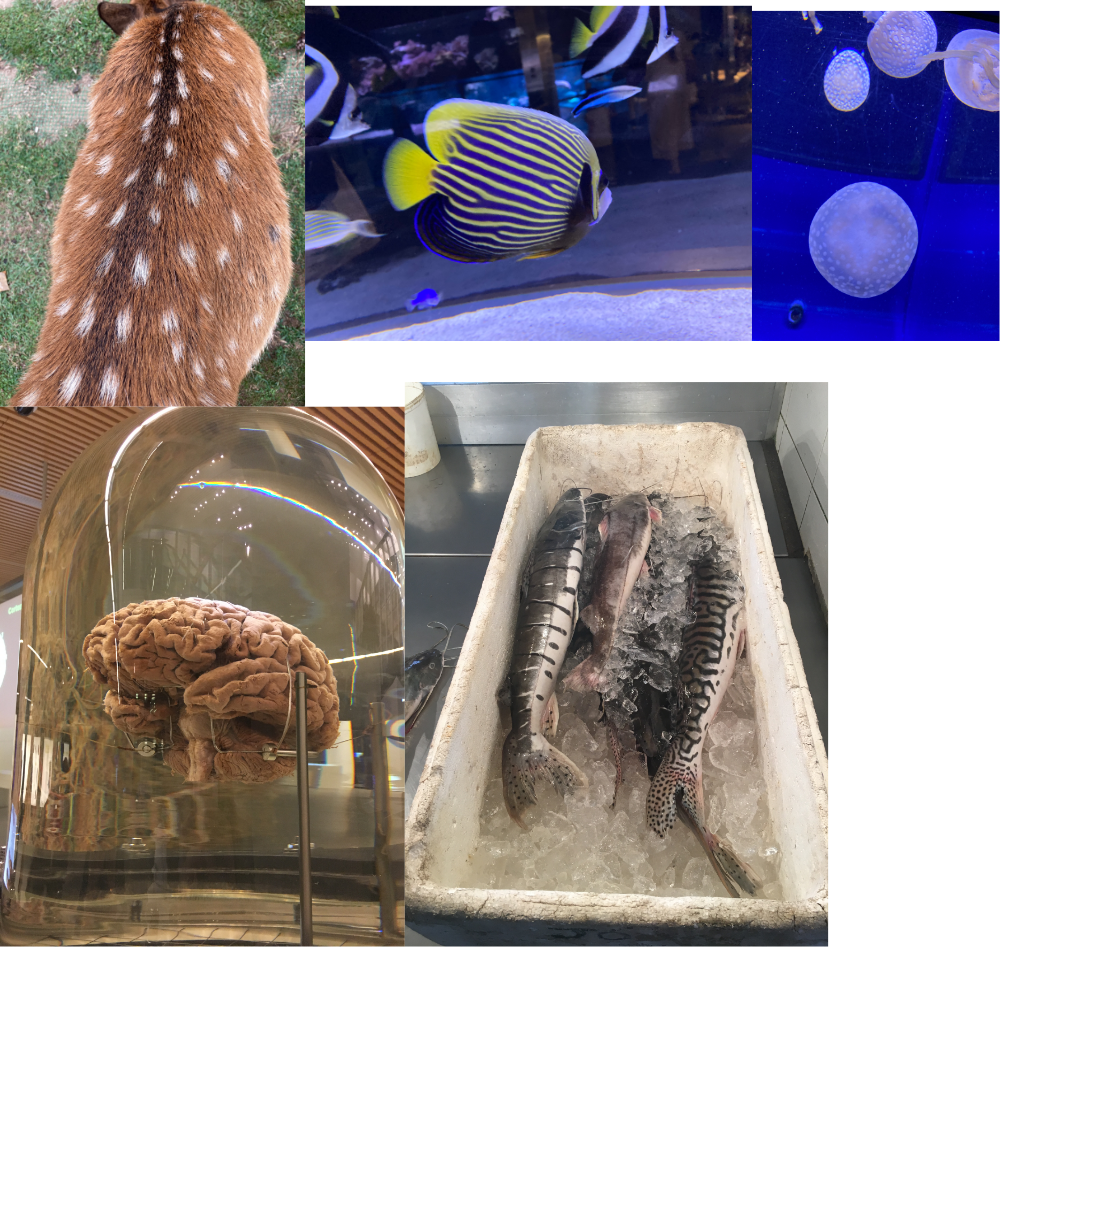
\includegraphics[width=1\textwidth]{chapters/Introduction/pattern_examples}
    \caption[\textbf{Examples of Turing patterns in nature.} ]{\textbf{Examples of Turing patterns in nature.}}
    \label{fig:pattern_examples}
\end{figure}
%todo add all pattern images and the respective species if available
This evolution from simplicity to intricacy isn't merely aesthetic; it often plays a pivotal role in the functioning of multicellular beings.
Delving deeper, these patterns can have strategic advantages.
Fractal-shaped bacterial colonies, for instance, maximise nutrient absorption ~\parencite{Matsushita1990}.
Furthermore, distinct colorations, such as the zebra's stripes or the mesmerising eye-spots on butterfly wings ~\parencite{Blest}, serve to disorient predators; either by disrupting the prey's silhouette or suggesting the prey is part of a larger entity ~\parencite{Stevens2006}.
The spirals observed in phylotaxis offer plants a way to optimise sunlight capture, enhancing photosynthesis ~\parencite{Strauss2020}.

The evolutionary advantage conveyed by this level of spatial organisation  hints towards genetic networks being potentially responsible for the patterning mechanism.
A randomly found solution of evolution where a pattern occurs, could lead to the genetic networks driving these spatial arrangements to be evolutionary beneficial and therefore selected.
Comprehending these networks and the dynamics that lead to these spatial designs is essential.
This area of research not only tries to understand which genetic networks and mechanisms are behind patterning.
It also seeks to uncover how on a molecular scale these mechanisms are reliable, accurate and robust to the noisy and exposed biological environment.
Additionally, studying this goes beyond understanding of developmental biology and morphogenesis.
It paves the way for pioneering work in biotechnological sectors, enabling the creation of intricately patterned tissues, efficient biofilms, or even organoids that hold potential in groundbreaking applications, such as tissue regeneration or organ implants ~\parencite{Scholes2017,Tan2018}. %todo comment on material deposition.



\subsection{Patterning theories}
Numerous mechanisms have been proposed in the literature to explain the formation in biological spatial systems.
Some of the most relevant ones can be categorized into mechanical instabilities and diffusion-based mechanisms %~\parencite{kosmrlj2020_2}.
The mechanical instabilities include phenomena such as differential adhesion, branching or wrinkling where physical forces are described in the model~\parencite{Scholes2017}.
% TODO SEARCH OTHER INSTABILITIES %todo cite other mechanical instabilities papers
On the other hand, gradient or diffusion based mechanisms rely on cells in the tissue responding to a molecule which is spatially heterogeneous and therefore exhibiting different phenotypes in different regions of the tissue (e.g.\ black vs white in zebra).


\section{Reaction-diffusion systems}
\subsection{Types of reaction diffusion: Wolpert vs Turing}
Among these gradient-based mechanisms, notable examples include positional information, the clock-and-wavefront model, and Turing instabilities ~\parencite{Wolpert1969, Baker2006, Turing1952}.
Both the positional information and clock-and-wavefront concepts are underpinned by an initial gradient of morphogens, interpreted by a genetic network to induce tissue patterns.
Sometimes, the origins of this gradient can be attributed to external factors such as ambient temperature, maternal impacts, or light exposure ~\parencite{Schier2009}.
However, in specific instances, the presence of an initial pre-pattern might be implausible, raising questions about how patterns spontaneously emerge from a prior uniform tissue.
Addressing this conundrum, the Turing's model offers an alternative as it doesn't need a pre-existing gradient and is self-organising ~\parencite{Kondo2010a}. %comment on space scaling, repetitive patterns and wide variety of shapes. check if the others can do it... i think not easily.
Given its attributes, the reaction-diffusion model might provide a more complete answer to the question of patterning in biology/ more holistic perspective on the intricacies of morphogenesis.
For this reason, Turing's mechanism for pattern formation will be the main focus of this work.
Nevertheless, it's pivotal to recognize that these mechanisms aren't strictly independent of each other.
The intricate nature of biological patterning might be best elucidated by an amalgamation of these theories, suggesting a blended framework may hold the answers ~\parencite{Green2015}. %todo discuss turings comment Turing himself recognized the biological unreality of this in stating that 'most of an organism, most of the time is developing from one pattern to another, rather than from homogeneity into a pattern' 1-34]
% TODO comment more on the fight between wolpert and turing and on the french flag model in general
\subsection{Turing patterns}
Reaction-diffusion systems were originally introduced in 1952 by Alan M. Turing in his paper “The chemical basis of morphogenesis” ~\parencite{Turing1952}.
In this article, he argues that pattern formation can be obtained when two morphogens interact with each other and diffuse at different
velocities across a tissue.
Morphogens, which are small molecules that can travel across the tissue and activate or inhibit other molecules.
If these morphogens are linked to growth hormones or skin pigments, biological patterns leading to a phenotype can arise.
The resulting patterns, called Turing patterns (TPs), can have different shapes such as stripes, labyrinths, spots; which can be widely observed in natural systems.
The concept of Turing patterns was first introduced from a mathematical perspective and was modelled using space and time dependent partial differential equations (PDE). In the case of Turing’s seminal paper, the set of PDEs describes a two node network (Fig. ~\ref{fig:intro_to_turing_patterns}A) which has activation and inhibition terms, degradation terms and diffusion terms (Fig.~\ref{fig:intro_to_turing_patterns}B).
The key feature of this system is that it can exhibit diffusion driven instabilities: Initially, the tissue has a homogeneous concentration of morphogen under which no diffusion occurs, and under these circumstances the system is stable and converges into an equilibrium state.
When biological noise is introduced, the heterogeneity of the system leads to morphogen diffusion.
Consequently, the diffusion leads to changes in the reaction rates and the system is pushed out of steady state leading to an unstable system.
This unstable system converges into a stable stationary periodic pattern which is a Turing pattern (Fig.~\ref{fig:intro_to_turing_patterns}C.
This whole phenomenon called the diffusion-driven instability is the essence of Alan Turing’s paper and one of the most used mechanisms to explain morphogenesis.

\begin{figure}[h!]
    \centering
    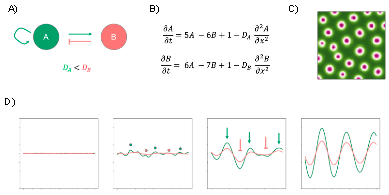
\includegraphics[width=1\textwidth]{chapters/Introduction/intro_to_turing_patterns}
    \caption[\textbf{Introduction to Turing's mechanism of pattern formation}]{\textbf{Introduction to Turing's mechanism}. \textbf{(A)} 2 node network based on Turing's original paper. Slow diffusing activator in green and fast diffuser inhibitor in pink. \textbf{(B)} Linear PDE equations for a 2-node Turing system. \textbf{(C)} 2D simulation of equations in B) using ADI numerical solver (See Methods \ref{ADI}). \textbf{(D)} }
    \label{fig:intro_to_turing_patterns}
\end{figure}
%TODO rerun simulations  1D snapshots and video


\subsection{Gierer-Meindhardt model}
Altough Turing’s work was of key importance in the field of developmental biology, it was not well accepted by biologists due to different reasons.
Firstly, the mathematical complexity behind it made it inaccessible for many scientists in the field.
Furthermore, the network proposed, although it can generate patterns, is too simple to describe the complexity in biological systems and takes some unrealistic assumptions such as the presence of negative concentrations ~\parencite{Kondo2010a}.
To solve these two issues, Gierer and Meindhardt proposed a generalised version of Turing’s diffusion-driven-instabilities ~\parencite{Gierer1972}.
This alternative theory proposes that patterns can be obtained as long as short-range activation and long-range inhibition (SALI) is present.
This implies that we can go away from Turing’s equations and extend the theory to networks with different number of nodes, different network interactions and even different signal transduction mechanisms ~\parencite{Murray1983, Rauch2004, Swindale1980}.
This step was necessary to be able to attribute patterning phenomena to more complex cellular and molecular interactions described by non-linear terms and larger networks with more nodes involved.
Examples of the first systems developed with non-linear terms are the typical Gierer-Meindhard model ~\parencite{Gierer1972}, Schnakenberg model ~\parencite{Schnakenberg1979}, as well as the Thomas model %~\parencite{thomas1976analysis}.
This generalisation work, sheds some light into the logic behind patterning and allows to understand it intuitively:
As an initially homogeneous system is perturbed by biological noise, local peaks of a morphogen concentration form.
These transient peaks lead to a local activation effect where the concentration of all reactants increases.
Due to the difference in diffusivity, the inhibitor reaches further away and long range inhibition is achieved.
Ultimately, this system settles into a stationary pattern with activation peaks and inhibition troughs ~\parencite{Gierer1972}.
This SALI mechanism proposed in this paper can be better understood in Figure ~\ref{fig:intro_to_turing_patterns}D.
%todo maybe add more detail from detailed explanation: Imagine a system with two chemicals: an activator and an inhibitor. The activator stimulates its own production, that of the inhibitor, and the production of black pigment. The inhibitor, however, reduces the production of both activator and black pigment.This simple network leads to regular patterns when diffusion is introduced: these chemicals can spread, but they don't travel at the same speed. The activator moves slowly, affecting only nearby areas, while the inhibitor travels faster, reaching farther areas. As the activator starts working, a local region of black is produced. Some inhibitor is also produced, which travels faster than the activator, reaching further away and leading to inhibition and white in the areas surrounding the black. Once the inhibitor's effect diminishes in a distant region, the activator becomes dominant again, leading to another spot of pigment production. The repetition of this event across the tissue results in regular spots or stripes of pigment. These are the principles underpinning Alan Turing’s theory of pattern formation known as “Turing patterns”, which explain regular pattern formation in biology.

\subsection{Turing patterns in nature}\label{Turing patterns in nature}
Various links have been made between biological patterns found in nature and Turing patterning networks.
As a basic example, seashell pigmentation and various types of fish skin have been replicated using simulations of Turing pattern systems.
Additionally, perturbation experiments in zebrafish’s skin are consistent with simulations of RD equations where the pattern regenerates in the exact same way after being physically disrupted both \textit{in-vivo} and \textit{in-silico} ~\parencite{Kondo2010a}.
Perturbation experiments are also carried out in the mammalian palatte, providing evidence of a Turing-type reaction-diffusion mechanism %todo cite palatte {economou}
Finally, molecules involved in patterning and morphogenesis have been shown to be part of networks with SALI characteristics.
For example, hair follicle development and fingerprint formation have been shown to rely on the same Turing reaction-diffusion network, based on signaling between EDAR, WNT, and antagonistic BMP pathways ~\parencite{Glover2023}
Other examples of Turing SALI networks are Nodal \& Lefty in right left asymmetry ~\parencite{Nakamura2006}, Bmp \& Sox9 \& Wnt in limb digit development ~\parencite{Raspopovic1} and finally Wnt \& Dkk involved in lung branching ~\parencite{langhe2005_lung}.
All these examples of the relationship between biological patterns and RD systems, SALI networks and diffusion-driven instabilities strongly suggest that the Turing mechanism is linked to the self-assembling and self-regenerative patterns observed in nature.
However, the arguments mentioned above make Turing’s mechanism purely a strong hypothesis of patterning and do not prove causation.


%todo Feather patterning appears to similarly combine these mechanisms - reaction diffusino with cell movement (Ho et al.,2019).

%%todo add Recent experimental findings (Raspopovic et al., 2014; Junget al., 1998; Sick et al., 2006; Economou et al., 2012; Nakamasu et al., 2009) have resulted in Turing patterns being widely accepted as an important mechanism for spatial patterning in developmen-tal processes.

%
\section{Mathematical analysis of Turing patterns}

\subsection{Analysing Turing patterns}
Turing patterns are commonly studied using mathematical tools to understand their features and behaviours.
The equations describing these reaction-diffusion systems are usually too complex to solve analytically as they contain non-linearities and partial differential terms.
For this reason, different methods must be used such as linear stability analysis (LSA) or numerical methods.
LSA provides information on how the stability of the system evolves as we go from a system without diffusion to a system with diffusion ~\parencite{Glendinning1994}.
For RD systems to produce Turing patterns, they must be stable without diffusion and become unstable as diffusion is turned on ~\parencite{J.DMurray2002}.
This stability profile gives rise to the name “diffusion-driven instabilities” which is an alternative name for Turing patterns.
Overall, this method can tell us whether a system is a pattern generator, the wavelength and the relative speed of pattern formation.
Alternatively, numerical methods are used to calculate the concentration of species in the RD system at every time and space point ~\parencite{Ramos1983}.
A visual solution is obtained which provides information on the shape, wavelength, evolution and amplitude of the pattern.
While numerical methods provide more information than LSA, they are more computationally expensive and can lead to numerical errors ~\parencite{J.DMurray2002}.

In terms of the computational power and time required, recently developed tools such as VisualPDE can make it easier and faster to explore and get intuition on the numerical solutions a system ~\parencite{Walker2023}.
Both have their advantages or disadvantages and must be used in combination for an optimal study of RD systems and patterning.
\subsection{Fine-tuning problem}

Using both linear stability analysis and numerical methods, Turing patterns were widely studied to understand whether they were a plausible explanation for pattern formation in biology.
Although patterns were obtained analytically and numerically using models of the SALI networks mentioned above, the fine-tuning problem makes this mechanism questionable.
The fine-tuning problem or robustness problems refers to the small fraction of the parameter space leading to Turing patterns and high sensitivity to parameter changes.
This issue was widely explored in ~\cite{Scholes2019}, where the parameter space of all 2-node and 3-node networks were studied using LSA to check for Turing patterning.
It was found that although 61\% of the networks can produce Turing patterns, only 0.1\% of the parameter space is within Turing space.
Similar results were obtained in ~\cite{Zheng2016} and ~\cite{Marcon}.
To comment further into parameter tuning, original 2-node reaction diffusion systems require large differential diffusion rates between the two morphogens as explained previously for SALI mechanism to occur.
This is sometimes biologically unlikely, as many of the morphogens have similar diffusion rates due to their similarities in molecular size ~\parencite{huidobro}.
Finally, turing patterns can sometimes be sensitive to the initial conditions, leading to different patterns.
This is problematic as developmental biology expects robust patterns as cells need to respond to specific queues.   %todo find ref for this.

Another issue with Turing patterns is the sensitivity to the initial conditions.
Although the shape of the pattern is not strictly determined by the initial conditions, finer details like locations of spots and stripes can be influenced.
Additionally, although the final pattern is the same, the transient dynamics might differ between different initial conditions (e.g.\ different transient pattern or convergence time before settling into the final pattern).
This can be an issue as in developmental biology, is a tightly controlled process where cells must receive the exact same signals in the same location and time to robustly reproduce the pattern. %todo find ref for this.





\subsection{Robustness of Turing patterns in realistic systems: bigger networks, growth, boundaries, noise, agar thickness}
On one hand, Turing's mechanism seems to explain many different patterns in biology as well as their perturbation experiments.
On the other hand, it does not seem a very robust mechanism.
How do these two contradicting ideas come together?
How can we make patterns more robust?
Typically, turing patterns are often studied in non-realistic systems.
A new direction in the field aims to study Turing patterns in more realistic systems large networks, systems with cooperativity, tissue discreteness at the cell level, growth, different boundary conditions, noise, delays, agar thickness.
Surprisingly, some of these realistic biological conditions increase robustness for Turing pattern formation. %Studying Turing patterns with a more biological point of view can potentially help solve the robustness issue.

\subsubsection{Large networks}
Biological networks usually far from the idealised 2-node Turing networks. %todo quote average network size
Recent studies ~\parencite{Zheng2016, Scholes2019, Marcon} have shown larger networks exhibit greater robustness to parameter variations.
Specifically, it has been shown that adding an immobile substrate to a 2 node diffusible system relaxes differential diffusion constraints expected in the classic SALI topologies ~\parencite{korvasova2015}.
However, studying large networks is very computationally expensive because of various reasons including exponential increase in possible networks, increase in dimensions of the parameter space, increase in number of equations.
This has resulted in limited studies addressing larger networks than 3.
~\cite{Smith2018a} tackles this challenge by simplifying big networks into smaller ones.
The reduced model is not an accurate description of the original system.
However it can predict whether a system will not show instabilities, ruling out many cases to study and reducing the computational cost of exploring larger networks.
~\cite{Haas2021} studies large networks with six diffusers using a random matrix approach and also shows that there is a relaxation in differential diffusion constraints.
This linearised random matrix approach previously used in ecology ~\parencite{May1972} could be used to explore large networks with mostly non-diffusible components that resemble the scale of real biological networks. %todo cite may without caps
%todo move somewhere else %Increase in robustness, and specifically decrease in differential diffusivity constraints is key to engineer biological pattern formation, as many available diffusers available in synthetic biology are predicted to diffuse at roughly equal speed due to their similarities in molecular weight ~\parencite{huidobro, Kondo2010a}

\subsubsection{High cooperativity}
Gene networks are usually described using non-linear Hill functions as many transcription factors exhibit allosteric behaviours in DNA binding ~\parencite{Morgunova2017}.
Greater cooperativity, reflected in steeper dose-response curves, can expand the Turing parameter space region and reduce the constraints imposed by differential diffusivity ~\parencite{Diambra2015a}.
%\subsubsection{Robust topologies}
%Studies have identified specific network topologies that exhibit enhanced robustness ~\parencite{Scholes2019}, which can be used when engineering patterns in synthetic biology. Nature probably converges into those topologies to maximise pattern formation robustness. The most robust topologies found in ~\cite{Scholes2019} are in line with the design principles found in other studies ~\parencite{Zheng2016} which show coherent activation and inhibition increases robustness.
%
%
%\item robust topologies and motifs: most robust topologies found in ~\parencite{Scholes2019}. This topology is in line with design principles
%found in other robustnes papaers try using as many AIJT topologies in the network as possible (coherent activation and inhibition) 2node core activation inhibition topology. ~\parencite{Zheng2016}. adding immobile no®de ~\parencite{Zheng2016,Diego2018} reduces need for differential diffusion.  %todo cite scholes most robust topology, msc thesis. %

\subsubsection{Discrete models}
Using discrete models can also show an increase in robustness.
Discretising concentration levels in ~\cite{Leyshon2021} which results in states rather than continuous kinetics, leads to some topologies being more robust to pattern formation. %todo justification of this discretisation.
Additionally, discretising space to cell size can lead to pattern formation in certain systems that usually do not allow it such as single diffuser networks ~\parencite{Wang2022}.

 % discrete models (discrete lattice gas cellular automaton (LGCA) framework.)concentration discreetenes: it confines the concentrations to a small number of discrete values (four in our case) and comprises discrete maps between these states rather than continuous kinetic parameters.Moreover, we found these five topologies to be more robust in the LGCA framework than they appear to be in the continuous case. ~\parencite{Leyshon2021}
 \subsubsection{Growth}
Fixed domains are often commonly assumed in developmental biology, as pattern forming processes (e.g reaction-diffusion of chemical species) occur at a much faster timescales than tissue growth. %todo add ref    %ref turing, ref 3 atlas papers
However, models of pattern formation in growing domains have shown growth to be extremely important in the development and morphology of the pattern.
Biological examples include angelfish \textit{Pomacanthus imperator} where growth induces the addition of new stripes in a branching point, while a constant wavelength ~\parencite{Kondo1995}.
In synthetic systems, the importance of growth can also be observed using a chemical reaction-diffusion system that grows over time ~\parencite{Konow2019}.
Slow growth rates were likely to produce rings added on the inside of the disk as it grew (inner ring addition), while fast growth rates produced rings on the outside (outer ring addition).
Intermediate growth rates formed labyrinthine structures.
All these principles of pattern morphology and growth rate are verified in the model.
These biological examples of growing patterns highlight the importance of including growth in models of pattern formation and specifically Turing patterns.

Considering the importance of growth in pattern morphology, it is key to consider how this growth might affect parametric robustness in Turing pattern formation.
Interestingly, introducing slow isotropic growth allows certain network topologies to form Turing patterns, which would not without growth.
An example of that is patterns in activator-activator networks, showing growth induced Turing instabilities.
Additionally, short-range activation and long-range inhibition can also produce Turing patterning in growing domains ~\cite{gaffney2010}.
Finally, increasing growth rates can increase the Turing parameter space under exponential growth in Turing patterning networks.
However, the analytical analysis used in ~\cite{gaffney2010} only holds when assuming slow isotropic growth and will break under faster growth.

Under logistic and linear growth, the Turing parameter space also changes.
However, the analysis used in ~\cite{gaffney2010} only holds when assuming slow isotropic growth and will break under faster growths.
This analysis is revisited in ~\cite{Klika2017} where they manage to study faster isotropic growing domains.
However, they observe that the conditions for Turing instabilities are more complex with higher growth rates and therefore more challenging to study than the ones in ~\cite{gaffney2010}.
This complexity makes it difficult to carry out high throughput studies of robustness and Turing parameter space in growing domains.
Finally, other types of growth such as anisotropic growth ~\parencite{Krause2019} are studied, but again they do not study parametric robustness in detail.

\subsubsection{Boundary conditions}.
Biological systems can exhibit a wide variety of boundary conditions depending on the context and environment.
Additionally, these boundary conditions can also be replicated using techniques in synthetic biology ~\parencite{Krause2020, Sheth2012, Vahey2014}.
Different theoretical studies explore a wide variety of boundary conditions for Turing systems.
Initially, it was shown that non-homogeneous boundary conditions where the system is not insulated, are less sensitive to changes in the domain size, different initial conditions and perturbations in model parameters ~\parencite{Arcuri1986}.
Then, mixed boundary conditions where different species are subject to different boundary definitions were also shown to increase parametric robustness ~\parencite{Maini1993, Maini1997, Krause2021}.
Studying these effects of these boundary conditions analytically is relatively complicated as you need to understand the bifurcation from which the Turing instability arises.
For example, although a Turing bifurcation is canonically a pitchfork bifurcation under Neumann boundary conditions, the Turing bifurcation is canonically a transcritical bifurcation under Dirichlet boundary conditions ~\parencite{Woolley2022}. %todo look at this again
This shows how much effect the boundaries have on the Turing instability, meaning they need to be considered when studying such systems.
An more applied biological example of how boundaries can affect pattern formation is seen in ~\parencite{Krause2020} where they study patterning synthetic biofilm in agar plates.
In this case, the agar absorbs the diffusers through the boundary, disrupting the pattern formed in the biofilm.
This effect can be reduced by decreasing the thickness of the agar layer.
Potentially, the pattern could also be maintained by reducing the permeability of the agar through the introduction of a filter paper or reduction of pore size.

%todo add robustness upon prepatternur

%
%Indeed, the idea that biological systems exchange material with their immediate environment seems likely in many situations. Therefore no-flux boundary conditions might be irrealistic.
%(point sources in butterfly wings %todo cite murray 1981)

%    also boundary between two different types of cells may give rise to morphogen production at the boundary interface %todo ~\parencite{meinhardt1981}.





\subsubsection{Noise}
Biological systems are known for their inherent noise.
In certain non-Turing parameter regimes, noise can drive diffusion-driven instabilities.
If there is a stable mode with eigenvalues slightly below zero, noise can destabilise this mode leading to a noise-induced instability and therefore the emergence of a pattern.
This might be a source of parametric robustness, producing patterns where deterministic systems do not predict one ~\parencite{Butler2009, Butler2011, Biancalani2010}.
Additionally, stochastic Turing patterns do not require large differential diffusivity between activator and inhibitor.
However, these patterns are not as ordered as deterministic Turing patterns ~\parencite{Karig2018}.
In terms of morphological robustness, deterministic Turing patterns were subjected to intrinsic noise using the same parameter region, and it was shown analytically that stochastically excited wave modes correspond exactly to their deterministic analogues, leading to a similar pattern.
Additionally, since noise perturbs populations away from the steady state, patterns can form quicker in a stochastic system than its deterministic counterpart ~\parencite{Maini2012}


\subsubsection{Delays} Having talked about realistic biological effects that contribute to pattern robustness, gene expression delays have been shown to do exactly the opposite.
Transcription and translation are biochemical processes that can occur in the scales of minutes to hours (depending on the size of the genomic sequence).
Therefore, from a gene being activated to the protein being active, there is a delay that is often not accounted for when modelling patterning.
The pattern morphology has been shown to be extremely sensitive to delays including sensitivity to the initial conditions in the final pattern, dramatic changes in the patterning lag under different delays and even pattern loss when delays are introduced ~\parencite{Maini2012}.


Overall, it is important to understand how different phenomena can affect pattern formation and introduce in models the most relevant to the natural system or experimental system being studied.
Furthermore, in some cases, these biological phenomena could increase robustness to pattern formation and explain the lack of robustness found in classical Turing pattern studies ~\parencite{Scholes2019}.
%
%\item turing instability can appear through a pitchfork bifurcation (subcritical ) ---> l (Leppänen 2004; Benson et al. 1998;Crampin 2000;Dutt 2010, 2012; Grindrod 1996; Nicolis 1995; Auchmuty and Nicolis 1975; Bozzini et al. 2015; Breña-Medina and Champneys 2014; Dalwadi and Pearce 2022).  transcritical bifurcation
%Critically, the changes in bifurcation structure that are produced by altering the
%boundary conditions from Neumann to Dirichlet are not observed in the linear analy-
%sis,In this paper, we rectify this situation by demon-
%strating that although the Turing bifurcation is canonically a pitchfork bifurcation
%under Neumann boundary conditions (van Hecke et al. 1994), the Turing bifurcation
%is canonically a transcritical bifurcation under Dirichlet boundary conditions



\section{ Engineering reaction-diffusion patterns}
There are various reasons to justify the engineering of Turing patterns in biology.
These justifications span from enhancing our fundamental understanding of how patterns develop in living organisms to the potential advancements these synthetic structures could contribute to biotechnology.
To begin with, there is a wealth of biological patterning that is associated with Turing-like gene networks, as indicated by numerous studies referenced in ~\ref{Turing patterns in nature}.
However, due to the tangled nature of biological systems, it is extremely hard to prove a Turing’s mechanism is actually behind those biological patterns.
Building a synthetic pattern based on the principles of Turing's mechanism would prove this mechanism can indeed form patterns in biology.
Furthermore, the integration of Turing patterns with real biological scenarios involving growth, stochasticity, or different boundary conditions could shift theoretical models towards more robust patterns that resemble more closely those found in nature.
Finally, the synthetic patterns obtained would contribute to novel nanotechnologies, such as systems with patterned biomaterial deposition ~\parencite{Din2020, Cao2017}.
For this reason, a bottom-up approach is required to build a system from first principles, which is tunable and insulated from the tangled genetic context, and which can be used to build tissues of interest.



\subsection{Previous work on engineering spatial patterns}

Engineering Turing patterns in biology is a highly challenging endeavour that has required synthetic biology to gradually develop the appropriate tools.
This has involved creating simpler biological patterns, as well as chemical Turing patterns to gain the necessary insights and tools for this complex task.
In synthetic biology, a wide variety of pattern generators have been engineered ranging in different complexities and pattern outcomes.
To systematically categorise these synthetic patterning systems, we can group them into four levels based on design characteristics ~\parencite{huidobro}:

Level 0 circuits lack synthetic signals that diffuse through normal Fickian diffusion, where the molar flux due to diffusion is proportional to the concentration gradient.
Instead, spatial structures emerge from other processes like cellular growth nd gene expression freezing.
Examples include synchronised oscillator circuits in bacterial colonies producing periodic concentric ring patterns without diffusing signals ~\parencite{Potvin-Trottier2016, Riglar2019} (See Fig. \ref{fig:engineered_patterns} Level 0).

Level 1 circuits do rely on diffusible components; however, these are not dynamically regulated, meaning they are not produced by the circuit as it is in the case of Turing patterns.
These diffusers only act as a pre-pattern which the system will interpret ~\parencite{Basu2005, Schaerli2014, Kong2017, Barbier2020, Grant2020}.
Although stripes and sharp boundaries can be obtained, their periodicity is limited.
Hierarchical patterning circumvents the periodicity issue by scaling level 1 systems ~\parencite{Boehm2018}.
More diffusers are added so $(2n-1)$ spatial domains can be generated with n orthogonal diffusers.
While hierarchical patterns can explain some developmental periodic patterns such as the neural tube in vertebrates ~\parencite{Briscoe2015}, it fails to capture the self-organising periodicity of Turing patterns observed in development such as digit patterning ~\parencite{Sheth2012,Raspopovic1} (See Fig. \ref{fig:engineered_patterns} Level 1).

Level 2 circuits do incorporate dynamically regulated diffusers; however, only one diffuser is introduced.
In contrast with level 1 systems, no pre-patterns are required to generate interesting behaviours.
Starting from a spatially homogeneous regime, these systems can produce robust spatial oscillators such as ~\parencite{Danino2010} or simple single ring patterns ~\parencite{Cao2016, Payne2013} (See Fig. \ref{fig:engineered_patterns} Level 2).

Finally, level 3 circuits use multiple dynamically regulated diffusible components (See Fig. \ref{fig:engineered_patterns} Level 3).
Turing patterns are the most prominent example of Level 3 systems as they as formed by reaction-diffusion circuits of at least two diffusers.
While numerous robust systems have been engineered in Level 0,1 and 2 circuits, Level 3 or Turing pattern engineering are still in its infancy.
Stochastic Turing patterns were recently engineered in E. coli with a circuit implemented according to the self-activation and lateral inhibition topology, with two diffusible quorum-sensing signals ~\parencite{Karig2018}.
Additionally, solitary patterns have also been engineered in a refactored Nodal–Lefty system in HEK cells ~\parencite{Sekine2018}.
While easier to engineer due to their relaxed fine-tuning requirements, stochastic Turing patterns and solitary display more irregularity in their periodic spatial structure ~\parencite{Butler2011, Karig2018,Sekine2018}.

While elusive in synthetic biology, regular-repeat Turing patterns have been engineered in chemical reaction systems.
They were first observed in the 1990's in the chlorite-iodide malonic acid (CIMA) reaction  ~\parencite{Castets, Lengyel1992} and later in the thiourea-iodate-sulfite (TuIS) reaction ~\parencite{Horvath} (See Fig. \ref{fig:engineered_patterns} Level 3).
Unlike biological systems, chemical reactions are reliably described by the simpler laws of mass action, and system parameters can often be identified ~\parencite{turanyi1994, kugler2009, Pusnik2019, Yeoh2019}.
Furthermore, the tuning of these systems by changing initial concentration or temperature has more predictable effects on the system ~\parencite{Horvath, landeira2010, Asakura2011}.
Lastly, chemical systems are isolated from external interacting components unlike biological systems where burden and cross-talk between the cellular chassis and synthetic parts is inevitable ~\parencite{Ceroni2015, Nielsen2016,Butzin2018, Du2020}.


Although chemical systems have helped understand pattern formation and could prove key to tissue engineering applications, mechanisms in biology seem to go beyond chemical systems.
Examples of patterns have been closely linked to gene expression patterns as shown in \textit{in-situ} hybridization studies ~\parencite{Jing2006}.
For this reason, it is key to explore this avenue and build genetically based reaction-diffusion systems that generate robust periodic patterns in biofilms.


\begin{figure}[H]
    \centering
    \includegraphics[width=1\textwidth]{chapters/Introduction/SpatialComponentsFigure1_300dpi}
    \caption[\textbf{Engineered spatial patterns in synthetic biology.}]{\textbf{Engineered spatial patterns in synthetic biology.} Four levels of regulatory complexity in engineered spatial patterning systems. Each level is divided into an example circuit, and the resulting pattern upon implementation. Diffusing components of the circuit are labelled with a “D”, non-diffusing nodes are unlabelled. The colour of each node corresponds to the colour of the reporter in the respective implementation. Level 0: synchronized repressilator circuit implemented in a growing bacterial colony \parencite{Potvin-Trottier2016}. The plot shows the circuit oscillations in single cells or stirred liquid culture. Level 1: incoherent feedforward circuit, where the diffusor-producing sender cells (cyan) are placed in the middle of a bacterial lawn ~\parencite{Basu2005}. The plot shows the concentration gradient of the diffusor away from the centre of the lawn. Level 2: self-activation and feedback inhibition circuit with one dynamically regulated diffusor creates spatial propagating waves and spatially synchronised oscillations (not shown) ~\parencite{Danino2010}. The plot shows the oscillations of the circuit in single cells, or in a cell population. Level 3: self-activation and lateral-inhibition circuit with two dynamically regulated diffusors creates stationary Turing patterns in the TuIS chemical system ~\parencite{Horvath}. The plot shows the localized, self-activating positive feedback of the slow-diffusing species D1 (blue curve) and the lateral inhibition of the fast-diffusing species D2 (yellow curve).} %TODO comment on adapted from literature
    \label{fig:engineered_patterns}
\end{figure}

%todo comment that patterns are linked to gene expression because Modern experimental interrogations of suspected mor-phogen-based pattern formation systems, such as Nodal and Lefty zebrafish mesendodermal induction,use in situ hybridization [24–26]. This explicitly highlights local concentrations of specific mRNA tran- scripts and thus provides an indication of the rates of transcription of target genes, and emphasizes the role of gene expression in morphogenesis. Chen, Y. & Schier, A. F. 2002 Lefty proteins are long-
%range inhibitors of squint-mediated nodal signaling. Curr.
%Biol. 12, 2124–2128. (doi:10.1016/S0960-9822(02)01362-3)
%25 Jing, X. H., Zhou, S. M., Wang, W. Q. & Chen, Y. 2006
%Mechanisms underlying long- and short-range nodal
%signaling in Zebrafish. Mech. Dev. 123, 388–394.
%(doi:10.1016/j.mod.2006.03.006)
\subsection{Engineering turing patterns in bacterial biofilms using exogenous circuit }
Even though they have been successfully engineered in chemical systems, the complexity of biology means that Turing patterns have never been engineered in a genetic context.
This can be attributed to the robustness problem including high sensitivity of parameters and a small fraction of parameter space producing Turing.
Additionally, designing Turing circuits with the classical 2-node topology leads to constrains in differential diffusivity that hinder the engineering of Turing patterns.
Finally, this fine-tuning issue is further amplified by the lack of orthogonal small-diffusible regulators to build a tunable synthetic pattering circuit.

All these issues have been addressed by previous researchers in the Isalan Lab and myself to achieve the engineering of a synthetic Turing circuit in bacteria that can produce regular periodic stationary patterns.
To address the fine-tuning problem and differential diffusivity constraints, ~\cite{Scholes2019} found that \("\)topology \(3954"\) (See Fig. \ref{fig:synthetic circuit} top-right) was amongst the most robust 3-node networks in terms of kinetic parameters.
Additionally, this topology allowed for equal diffusivity and even faster diffusing activators.
The lack of robust biological parts was addressed in ~\cite{Meyer2019} and ~\cite{Du2020} where orthogonal diffusers where characterized, which allow the building of the \("\)topology \(3954"\) topology.
These toolboxes are key to bridge the gap between abstract models and real-sender receiver circuits.
Additionally, in ~\cite{huidobro} we compiled a list of small molecule regulators that can diffuse and form gene circuits in e.coli, as well as their respective promoters and synthesis enzymes.
Finally, ~\cite{Tica2020} engineered the \("\)topology \(3954"\) using the components from ~\cite{Meyer2019} and ~\cite{Du2020} with the aim of exploring a robust Turing gene circuit for pattern formation (See Fig. \ref{fig:synthetic circuit} bottom).
Due to the lack of specific biological parts such as an inhibitor quorum sensing molecule or a dual inhibitor/activator molecule, the biological implementation of 3954 resulted in a six molecular specie circuit instead of the original 3-node network. 
In this thesis, theoretical work based on this synthetic gene circuit was carried out to understand how to tune parameters experimentally and what spatial setup to use to allow pattern formation in bacterial biofilms.
Additionally, once the setup is determined, to predict which patterns might appear and the relevant wavelengths to look for.
Finally, once patterns appear in the biofilm, to characterise and understand the mechanisms behind these patterns.
Having a genetic synthetic network that produces patterns with a predictive model would be extremely impactful on various levels.
Firstly, the model would allow us to understand the patterning mechanisms behind the synthetic system and therefore shed some light into developmental biology.
Currently, our understanding from top-down approaches is based on arbitrarily chosen models that match well the experiments, but that are not directly informed on well-known and characterised gene circuits.
In this bottom-up approach, the model used is derived from a known synthetic gene circuit that has been artificially introduced into cells. %TODO comment on bespoke turing patterns
If this network can produce self-assembling periodic stationary patterns, it would prove that reaction-diffusion patterns can form in biological systems supported by genetic interactions.
Secondly, it would allow us to inform the experimentalists on how to tune the system to obtain more robust desired patterns for tissue engineering in biotechnology applications.






\begin{figure}[H]
    \centering
    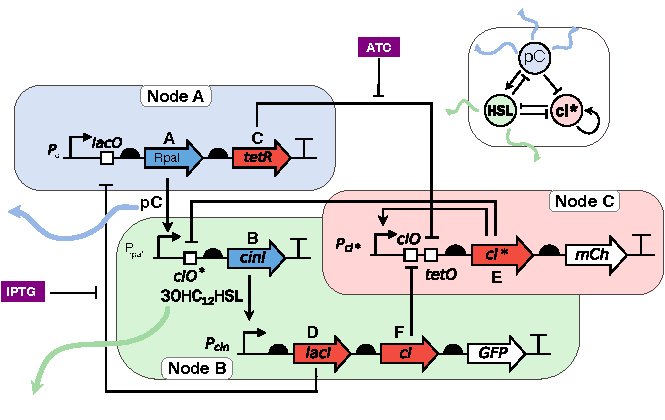
\includegraphics[width=1\textwidth]{chapters/Introduction/synthetic circuit}
    \caption[\textbf{Synthetic biology implementation of 3954) topology.}]{\textbf{Synthetic biology implementation of 3954 topology.} \TODO{Give more detail of this diagram}} %TODO give detail
    \label{fig:synthetic circuit}
\end{figure}




\section{Thesis overview}

%TODO
The aim of this thesis is to investigate Turing patterning in the context of synthetic biology and tissue engineering, using a modelling approach.
The first part of the thesis will take a more theoretical direction and do an in-depth investigation of how linear stability analysis relates to numerical solutions which themselves relate to the patterns seen in nature or experimentally.
This includes estimating wavelength, convergence time and in some cases pattern shape estimation from the dispersion relation.
Additionally, it also involves looking at which type of instabilities can produce stationary spatial patterns beyond Turing instabilities.
Going from this more theoretical approach, I will then consider realistic biological phenomena in the context of pattern formation such as different boundary conditions and growth.
Understanding how these phenomena affect pattern formation and its robustness, is key to understand which route to take when engineering pattern formation using synthetic gene circuits.
The second part of the thesis will focus on building a predictive model that can inform the experimental work in order to build a successful Turing pattern generator using gene circuits.
First, I will build a PDE system that describes the synthetic gene circuit engineered in ~\parencite{Tica2020}.
Then, I will explore the parameter space of this system to understand which regions are more robust in terms of pattern formation and how we can experimentally tune the genetic circuit in order to obtain a robust pattern generator.
Additionally, I will perform experiments where I grow small colonies with the synthetic gene network and image them using microscopy to observe fluorescence rings.
This experiment is continued by Jure Tica, Tong Zhu, Georg Wachter in larger colonies to observe a wide variety of patterns, including different types of stripes, spots and wedges.
Following this, I went on to develop a PDE solver combined with a cellular automata to model bacterial colony growth which I used to replicate all the patterns found.
Finally, the model is parametrised using minimisation and multivariate gaussian analysis, to constrain the parameters to more experimentally realistic values.
Inside the new parameter region, I find regimes which also produce Turing patterns, and more specifically the stationary rings observed.

%TODO write one sentence summary of value of this thesis


    \chapter{Theoretical study of Turing patterns }
\section{Synopsis}
When studying regular pattern formation in biology, Turing patterns (TPs) are a commonly used mechanism.
Studying TPs can be done both using linear stability analysis or numerical methods.
Linear stability analysis predicts whether a pattern will occur through a dispersion relation.
Although faster, this method provides less insights into the pattern that emerges, as it relies on the mineralisation around the steady state.
On the other hand numerical methods, which are more computationally expensive, provide a result detailed result which resembles the biological pattern. From this we can understand pattern shape, evolution, concentrations\ldots etc.
In this chapter, we first study the relationship between the analytical dispersion relation and the numerical results in TPs.
This includes understanding how to predict wavelength,
convergence time and even pattern shape from the dispersion relation.
This is important to circumvent expensive numerical methods to estimate some information from the emergent pattern without computing it numerically.
Then we explore how linear stability analysis might not always be a good predictor of pattern formation.
For example, how multistability can break linear stability analysis predictions and how other types of dispersion relation profiles or instabilities which are not classical Turing can generate stationary spatial patterns or other types of temporal-spatial patterns.
Finally, we explore numerically how these patterns behave when realistic biological systems from our experimental setup are introduced, including open boundaries or growth.



\section{Pattern information in the dispersion relation of Turing instabilities}
\subsection{Turing pattern's mathematical definition and the dispersion relation}


The following section describes how linear stability analysis is carried out for the equilibrium points in a reaction-diffusion system.
The aim of this analysis is to find out if the steady state exhibits a Turing instability or also called a diffusion-driven instability.
When it does, the system is capable of forming spatial patterns.
As the name describes, diffusion-driven instabilities arise in these systems when a homogeneous steady state is stable to small perturbations in the absence of diffusion, and becomes unstable in the presence of diffusion ~\parencite{Glendinning1994, J.DMurray2002}.
To check for Turing instabilities, the stability of the equilibrium state will be studied with and without diffusion.
The method of linear stability analysis will be explained for the two morphogen reaction-diffusion system, shown below:


\begin{subequations}
    \begin{equation}
        \pdv{A}{t}= f_{A}(A, I) + D_{A}\pdvn{2}{A}{x}
        \label{eq:RD general equation 1}
    \end{equation}
    \begin{equation}
        \pdv{I}{t} = f_{I}(A, I) + D_{I}\pdvn{2}{I}{x}
        \label{eq:RD general equation 2}
    \end{equation}
    \label{eq: RD general equations}
\end{subequations}
where $f_{A,I}$ are the non-linear production terms and $D_{A,I}$ are the diffusion constants of the two morphogens.
For future reference, X is a generalisation term to refer to any morphogen A or I.
\subsubsection{Stability of steady state without diffusion}
To study the stability around the steady state without diffusion (Eqs.\eqref{eq: RD general equations}) is used, except diffusion terms are removed ($D_{A,I}=0$):
\begin{subequations}
    \begin{equation}
        \pdv{A}{t} = f_{A}(A,I)
    \end{equation}
    \begin{equation}
        \pdv{I}{t} = f_{I}(A,I)
    \end{equation}
    \label{eq: R general equations}
\end{subequations}
The steady states are defined as $A^*$ and $I^*$, which satisfy the condition:
\begin{equation}
    f_{A}(A^*,I^*)=0, \hspace{1.5cm} f_{I}(A^*,I^*)=0
\end{equation}
Linear stability analysis is carried by adding an infinitesimally small perturbation $\delta X$ to the steady state $X^*$, and studying if the perturbation decays (stable steady state) or grows (unstable steady state) over time. The perturbation needs to be almost insignificant as Taylor expansion is carried out to linearise the system around the steady state. Therefore, the morphogen concentration can be expressed as:
\begin{subequations}
    \begin{equation}
        A(t) = A^* + \delta A(t),\hspace{1.5cm} |\delta A| <<A^*
    \end{equation}
    \begin{equation}
        I(t) = I^* + \delta I(t), \hspace{1.5cm} |\delta I| <<I^*
    \end{equation}
    \label{eq: steady states}
\end{subequations}
The differential Eqs. \eqref{eq: R general equations} are evaluated at steady state, using Eqs~\eqref{eq: steady states}:
\begin{subequations}
    \begin{equation}
        \pdv{A}{t} = \pdv{[A^* + \delta A(t)]}{t} = f_{A}(A^* + \delta A(t), I^* + \delta I(t)) = \pdv{\delta A}{t}
    \end{equation}
    \begin{equation}
        \pdv{I}{t} = \pdv{[I^* + \delta I(t)]}{t} = f_{I}(A^* + \delta A(t), I^* + \delta I(t)) = \pdv{\delta I}{t}
    \end{equation}
    \label{eq: R equations at steady state}
\end{subequations}
As previously mentioned, the non-linear system will be linearised around the steady state using Taylor expansion.
This is done to have a simpler set of equations, that represent the system around the steady state, as seen below:
\begin{equation}
    \begin{split}
         f(A^*+\delta A, I^*+\delta I) =  f(A^*,I^*) + \pdv{f(A^*,I^*)}{A}\delta A + \pdv{f(A^*,I^*)}{I}\delta I + \dots  \\\\ + \frac{1}{n!} \pdvn{n}{f(A^*,I^*)}{A}\delta A^n + \frac{1}{n!} \pdvn{n}{f(A^*,I^*)}{I}\delta I^n
    \end{split}
\end{equation}



%\begin{split}
%    \pdv{[X(x,t)]}{x}) = \mathcal{F}^{-1}\left(\pdv{[X(k,t)]}{x}\right) = \pdv{}{x}\left[\frac{1}{2\pi}\int_{-\infty}^{\infty} X(k,t)e^{ikx} dk\right] =  \frac{1}{2\pi}\int_{-\infty}^{\infty} X(k,t)\frac{d}{dx}e^{ikx} dk\\\\ =\frac{1}{2\pi}\int_{-\infty}^{\infty} ik X(k,t)e^{ikx} dk = ik \frac{1}{2\pi}\int_{-\infty}^{\infty} X(k,t)e^{ikx} dk = ik X(x,t)
%\end{split}




If $\delta A$ and $\delta I$ are small enough, higher order terms can be ignored as $\delta (A,I)^n$  becomes infinitesimally small.
Furthermore, it can be assumed that $f(A^*,I^*) = 0$, therefore the following expression is obtained, where $f$ corresponds to either $f_{A}$ or $f_{I}$  :
\begin{equation}
    f(A^*+\delta A, I^*+\delta I) =  \pdv{f(A^*,I^*)}{A}\delta A + \pdv{f(A^*,I^*)}{I}\delta I
\end{equation}
Finally, because $\pdv{X}{t} =  \pdv{\delta X}{t}$  at steady state (Eqs. \eqref{eq: R equations at steady state}), the change in perturbation, meaning decay or growth, can be expressed as:
\begin{subequations}
    \begin{equation}
        \pdv{\delta A}{t} = \pdv{f_{A}(A^*,I^*)}{A}\delta A + \pdv{f_{A}(A^*,I^*)}{I}\delta I
    \end{equation}
    \begin{equation}
        \pdv{\delta I}{t} = \pdv{f_{I}(A^*,I^*)}{A}\delta A + \pdv{f_{I}(A^*,I^*)}{I}\delta I
    \end{equation}
    \label{eq: linearised terms around steady state}
\end{subequations}


The general solution can be expressed as an exponential, where $\sigma$ determines the growth rate of the perturbation, and whether it grows (unstable steady state) or decays (stable steady state):
\begin{subequations}
    \begin{equation}
        \delta A = A_{0}e^{\sigma t}
    \end{equation}
    \begin{equation}
        \delta I = I_{0}e^{\sigma t}
        \label{eq: exponential R}
    \end{equation}
\end{subequations}
If Eq. \eqref{eq: exponential R} are introduced into  Eq. \eqref{eq: linearised terms around steady state} , and the solution divided by $e^{\sigma t}$ on both sides, the following is obtained:
\begin{subequations}
    \begin{equation}
        \sigma \delta A_{0} = \pdv{f_{A}(A,I)}{A} \delta A_{0} + \pdv{f_{A}(A,I)}{I}\delta I_{0}
    \end{equation}
    \begin{equation}
        \sigma \delta B_{0} = \pdv{f_{I}(A,I)}{A} \delta A_{0}+ \pdv{f_{I}(A,I)}{I}\delta I_{0}
    \end{equation}
\end{subequations}
This can be represented as an eigenvalue-eigenvector problem using the jacobian $\textbf{J}$, the eigenvalue $\sigma$ and the eigenvector  $\delta u_{X} = [u_{A},u_{I}]$:
\begin{equation}
    \sigma \delta X_{0} = \begin{bmatrix}
                              \pdv{f_{A}}{A} &
                              \pdv{f_{A}}{I}  \\
                              \pdv{f_{I}}{A} &
                              \pdv{f_{I}}{I}
    \end{bmatrix}\delta X_{0}
\end{equation}
Finally, $\sigma$ can be obtained by solving the characteristic polynomial:
\begin{equation}
    p(\sigma) = det[J-\sigma I] = 0
\end{equation}

The real part of $\sigma$ corresponds to the growth rate of the perturbation.
$Im(\sigma)$ corresponds to the oscillations.
If $Re(\sigma) < 0 $, the steady state will be stable to perturbations, which means the system will go back to steady state after a small perturbation is applied.
If $Re(\sigma) > 0 $, the steady state will be unstable to perturbations, and the system will go away from the equilibrium point after being slightly perturbed.
%
%-------------------
%
%This can also be written in terms of
%
%\begin{subequations}
%    \begin{equation}
%        \pdv{\delta A}{t} = a_{11}\delta A + a_{12}\delta I
%    \end{equation}
%    \begin{equation}
%        \pdv{\delta I}{t} =  a_{21}\delta A +  a_{22}\delta I
%    \end{equation}
%\end{subequations}
%
%where
%
%\begin{subequations}
%    \begin{equation}
%        a_{11} = \pdv{f_{A}(A^*,I^*)}{A} \hspace{1.5cm} a_{12} = \pdv{f_{A}(A^*,I^*)}{I}
%    \end{equation}
%    \begin{equation}
%        a_{21} = \pdv{f_{I}(A^*,I^*)}{A} \hspace{1.5cm} a_{22} = \pdv{f_{I}(A^*,I^*)}{I}
%    \end{equation}
%
%\end{subequations}
%
%It can also be expressed in terms of the jacobian J
%
%\begin{equation}
%    J = \begin{bmatrix}
%                              \pdv{f_{A}}{A} &
%                              \pdv{f_{A}}{I}  \\
%                              \pdv{f_{I}}{A} &
%                              \pdv{f_{I}}{I}
%    \end{bmatrix}
%    = \begin{bmatrix}
%          a_{11} &
%          a_{12} \\
%          a_{21} &
%          a_{22}
%    \end{bmatrix}
%\end{equation}
%
%For a vector U
%
%
%\begin{subequations}
%    \begin{equation}
%        U = \begin{bmatrix}
%                \delta A  \\
%                \delta I
%        \end{bmatrix},   \hspace{0.5cm}  \pdv{U}{t} = J \cdot U
%    \end{equation}
%\end{subequations}
%
%
%
%
%Diagonalisation can be applied to obtain an exponential solution for the perturbations $\delta A$ and $\delta B$ in terms of the eigenvalues $\sigma_{1}$ and $\sigma_{2}$ where $c_{1}, c_{2}, c_{3}, c_{4}$ are constants
%
%\begin{subequations}
%    \begin{equation}
%    \delta A(t) = c_{1}e^{\sigma_{1}t} + c_{2}e^{\sigma_{2}t}
%    \end{equation}
%
%    \begin{equation}
%        \delta I(t) = c_{3}e^{\sigma_{1}t} + c_{4}e^{\sigma_{2}t}
%    \end{equation}
%\end{subequations}


\subsubsection{Stability of steady state with diffusion}
Once the stability of the steady state has been analysed in the absence of diffusion, the effect of diffusion on the same system will be studied. The diffusion will be introduced through the partial derivative term $D_{X}\pdvn{2}{[X]}{x}$, where X is the morphogen in Eqs. \eqref{eq: RD general equations}.
\paragraph{Reduction of PDE term to ODE through Fourier transformations}
The second order partial derivative term will be reduced to an ODE simpler term through Fourier transforms. For this purpose, the following Fourier transform definitions are used:
\begin{subequations}
    \begin{equation}
        F(k) = \mathcal{F}(f(x)) = \int_{-\infty}^{\infty} f(x)e^{-ikx} dx
    \end{equation}
    \begin{equation}
        f(x) = \mathcal{F}^{-1}(F(k)) = \frac{1}{2\pi}\int_{-\infty}^{\infty} F(k)e^{ikx} dk
        \label{eq:inverse fourier}
    \end{equation}
\end{subequations}
First, using the inverse Fourier transform (Eq. \eqref{eq:inverse fourier}), the first order partial derivative will be reduced to an ODE form:
\begin{equation}
    \begin{split}
        \pdv{[X(x,t)]}{x}) = \mathcal{F}^{-1}\left(\pdv{[X(k,t)]}{x}\right) = \pdv{}{x}\left[\frac{1}{2\pi}\int_{-\infty}^{\infty} X(k,t)e^{ikx} dk\right] =  \frac{1}{2\pi}\int_{-\infty}^{\infty} X(k,t)\frac{d}{dx}e^{ikx} dk\\\\ =\frac{1}{2\pi}\int_{-\infty}^{\infty} ik X(k,t)e^{ikx} dk = ik \frac{1}{2\pi}\int_{-\infty}^{\infty} X(k,t)e^{ikx} dk = ik X(x,t)
    \end{split}
\end{equation}
giving $\pdv{[X(x,t)]}{x}) =  ik X(x,t)$.
Using this expression, the inverse Fourier transform and the fact that $\pdvn{2}{X(x,t)}{x} =\left(\pdv{X(x,t)}{x}\right)^2$, the following expression is obtained:
\begin{equation}
    \begin{split}
        \pdvn{2}{[X(x,t)]}{x}) = \left(\pdv{X(x,t)}{x}\right)^2 = \mathcal{F}^{-1}\left[\pdv{[ikX(k,t)]}{x}\right] = \pdv{}{x}\left[\frac{1}{2\pi}\int_{-\infty}^{\infty} ikX(k,t)e^{ikx} dk\right] \\\\=  \frac{1}{2\pi}\int_{-\infty}^{\infty} ikX(k,t)\frac{d}{dx}e^{ikx} dk =\frac{1}{2\pi}\int_{-\infty}^{\infty} (ik)^2 X(k,t)e^{ikx} dk = -k^2 \frac{1}{2\pi}\int_{-\infty}^{\infty} X(k,t)e^{ikx} dk = -k^2 X(x,t)
    \end{split}
    \label{eq:fourier of our system}
\end{equation}
giving
\begin{subequations}
    \begin{equation}
        \pdvn{2}{A(x,t)}{x} = -k^2\cdot A
    \end{equation}
    \begin{equation}
        \pdvn{2}{I(x,t)}{x} = -k^2\cdot I
    \end{equation}
    \label{eq: simplified fourier diffusion}
\end{subequations}
This way, the second order partial derivative terms, are reduced to simpler ODE systems to be used in linear stability analysis
\paragraph{Definition of boundary conditions}
The system is defined within some boundaries, meaning x goes from 0 to L. In this case, no molecules can leave the system, so the boundary condition applied is a zero-flux boundary condition. At the boundaries, the partial derivative is zero, defined below as Neumann Boundary conditions:
\begin{equation}
    \pdvn{2}{X(x=0,t)}{x}=0  \hspace{0.5cm}\And  \hspace{0.5cm}\pdvn{2}{X(x=L,t)}{x}=0
\end{equation}
This can be visualised as a fish tank, of length L, filled with water: water diffuses freely within the tank, but cannot diffuse outside the boundaries. In addition, the levels of water at the boundaries are not fixed. For the spatial derivatives to be zero at the boundaries, some restrictions will need to be applied. The expression from Eq. \eqref{eq:fourier of our system} will be used to apply our boundary conditions.
\begin{equation}
    \begin{split}
        \pdvn{2}{[X(x,t)]}{x}) =  -k^2 \frac{1}{2\pi}\int_{0}^{L} X(k,t)e^{ikx} dk =  -k^2 \frac{1}{2\pi}\int_{0}^{L} X(k,t)(cos(kx)+isin(kx))dk\\\\
        =\frac{-k^2}{2\pi}\left(\int_{0}^{L} X(k,t)cos(kx)dk + i\int_{0}^{L} X(k,t)sin(kx)dk\right)
    \end{split}
\end{equation}
The first integral is integrated by parts to express the equation in terms of $\sin(kx)$:
\begin{equation}
    \begin{split}
        \pdvn{2}{[X(x,t)]}{x}) = \frac{-k^2}{2\pi}\left(\left[\frac{sin(kx)}{k}X(k,t)\right]^L_{0} - \int_{0}^{L} \frac{sin(kx)}{k}\pdv{A(k,t)}{k}dk + i\int_{0}^{L} X(k,t)sin(kx)dk\right)
    \end{split}
\end{equation}
As defined with the boundary conditions (Equation 31), the partial derivative must be 0 at $x=0$ and  $x=L$.
Therefore, at $x=0$ and  $x=L$, $\sin(kx)=0$.
For the two boundary conditions:
\begin{itemize}
    \item When $x=0$: $\sin(k\cdot0)=\sin(0)=0$.
    \item Therefore for $x=0,\pdvn{2}{X(0,t)}{x}=0$.
    \item When $x=L$: $\sin(k\cdot L)$ must be zero.
    \item If $ k=\frac{n\pi}{L}$, $\sin(kL) = \sin(n\pi) = 0$.
    Therefore, for $x=L$ , $\pdvn{2}{X(L,t)}{x}=0 \hspace{0.5cm} \forall n \in \{0, \mathbb{N}\} $
\end{itemize}
Following these calculations, the zero-flux boundary condition is applied if the following condition is met:  ~$k=\frac{n\pi}{L} \hspace{0.1cm}\forall n \in \{0, \mathbb{N}\} $

\paragraph{Linear Stability Analysis of steady state with diffusion effects}
Now that the PDE diffusion term has been reduced to an ODE term, and the zero-flux boundary conditions introduced, the stability of the steady state when introducing diffusion can be studied.
As shown in Eqs. \eqref{eq: simplified fourier diffusion}, the diffusion term $D_{X}\pdvn{2}{X}{x} $ can be expressed as $-k^2X$, therefore the reaction-diffusion PDE equations are reduced to:
\begin{subequations}
    \begin{equation}
        \pdv{A}{t} = f_{A}(A,I)  -D_{A}k^2A
    \end{equation}
    \begin{equation}
        \pdv{I}{t} = f_{I}(A,I) -D_{I}k^2I
    \end{equation}
\end{subequations}
where $k=\frac{n\pi}{L} \hspace{0.1cm}\forall n \in \{0, \mathbb{N}\} $.

In the previous section, linear stability analysis was carried around the steady state with a perturbation $\delta X$, without including diffusion.
This resulted in the expression shown in Eq. \eqref{eq: linearised terms around steady state}, which describes the linearized reaction terms around the steady state.
By adding diffusion in the fourier domain from Eq. \eqref{eq: simplified fourier diffusion} we obtain the following expression for the linearized reaction-diffusion system:


\begin{subequations}
    \begin{equation}
        \pdv{\delta A}{t} = \pdv{f_{A}(A^*,I^*)}{A}\delta A + \pdv{f_{A}(A^*,I^*)}{I}\delta I  -D_{A}k^2\delta A
    \end{equation}
    \begin{equation}
        \pdv{\delta I}{t} =  \pdv{f_{I}(A^*,I^*)}{A}\delta A + \pdv{f_{I}(A^*,I^*)}{I}\delta I  -D_{I}k^2\delta I
    \end{equation}
    \label{eq:linearised RD}
\end{subequations}

We wish to find a general solution of the form:

\begin{subequations}
    \begin{equation}
        \delta A = A_{0}e^{\sigma t}\cdot e^{ikx}
    \end{equation}
    \begin{equation}
        \delta I = I_{0}e^{\sigma t}\cdot e^{ikx}
    \end{equation}
    \label{eq: exponential form RD}
\end{subequations}
where $X_{0}e^{\sigma t}$ represents the amplitude of the perturbations and $e^{ikx}$ represents the spatial oscillations (with $k$ as the wavenumber).
In this case, we are interested on the growth or decay of the perturbations over time.
Therefore, to observe the stability of the steady state, we will study the amplitude term ($X_{0}e^{\sigma t}$):
\begin{itemize}
    \item If $\sigma > 0$: perturbation ($\delta X$) grows making $\pdv{\delta X}{t} > 0$.
    Therefore, the steady state is unstable with diffusion.
    \item If $\sigma < 0$: perturbation ($\delta X$) decays making $\pdv{\delta X}{t} < 0$.
    Therefore, the steady state is stable with diffusion.
\end{itemize}
If Eqs. \eqref{eq: exponential form RD} are substituted into Eqs. \eqref{eq:linearised RD}, the following equations are obtained:
\begin{subequations}
    \begin{equation}
        \sigma \delta A_{0} = \pdv{f_{A}(A^*,I^*)}{A} \delta  A_{0}  + \pdv{f_{A}(A^*,I^*)}{I}\delta  I_{0} -D_{A}k^2\delta  A_{0}
    \end{equation}
    \begin{equation}
        \sigma \delta I_{0}= \pdv{f_{I}(A^*,I^*)}{A} \delta  A_{0}  + \pdv{f_{I}(A^*,I^*)}{I}\delta  I_{0}  -D_{I}k^2\delta A
    \end{equation}

\end{subequations}
These pair of equations can again be treated as an eigenvalue-eigenvector problem written in the following way:
\begin{equation}
    \sigma \delta X_{0} = \begin{bmatrix}
                              \pdv{f_{A}}{A} - D_{A}k &
                              \pdv{f_{A}}{I}  \\
                              \pdv{f_{I}}{A} &
                              \pdv{f_{I}}{I} - D_{I}k
    \end{bmatrix}\delta X_{0}
    \label{eq: jacobian RD}
\end{equation}
where $\sigma$ can be obtained by solving the characteristic polynomial:
\begin{equation}
    p(\sigma) = det[J-\sigma I] = 0
    \label{eq: characteristic polynomial RD}
\end{equation}
In summary, to understand if perturbations around the steady state decay or grow when diffusion is introduced, Eq. \eqref{eq: characteristic polynomial RD} must be solved to obtain $\sigma$.
This characteristic polynomial is solved for a range of k's, being $k=\frac{n\pi}{L} \hspace{0.1cm}\forall n \in \{0, \mathbb{N}\} $.
The sign of $\sigma$ is studied for every k, resulting in the dispersion relation %todo cite figure dispersion.
If $\sigma > 0$, perturbations grow around the steady state and the system is unstable.
In the contrary, if  $\sigma < 0$, the system is stable and perturbations decay around the steady state.
More detail on linear stability analysis can be found in~\cite{J.DMurray2002} or ~\cite{Glendinning1994}.
\subsubsection{Linear stability analysis implementation}
Linear stability analysis is carried out with and without diffusion for all steady states of the system found using Newton-Raphson method (See \ref{newton_raphson}).
The analysis is done for all $k=\frac{n\pi}{L} \hspace{0.1cm}\forall \{n \in \mathbb{N} : n \leq 5000\} $, meaning 5000 k's are sampled using linear stability analysis.
L is defined as 100mm which is based on the maximum lenght of our experimental system.
This system is further described in %todo mention chapter 2 and 3
Linear stability analysis for a single steady state takes approximately approximately 0.5s.

\subsection{Model definition and dataset creation}
The system studied in this chapter consists of a 2-node Turing topology system with non-linear hill terms.
The activator U activates itself and V, while the inhibitor V inhibits the activator U as seen in Fig. \ref{fig:intro_to_turing_patterns}A.
However, instead of using the linear terms used in the original Turing system Fig. \ref{fig:intro_to_turing_patterns}B ~\parencite{Turing1952}, we use Hill terms which represent genetic regulations.

\begin{subequations}
    \begin{equation}
        \pdv{[A]}{t}=b_{A}+V_{A} \cdot\frac{1}{1+\left(\frac{K{A}}{[A]}\right)^{n_{A}}}\cdot\frac{1}{1+\left(\frac{[I]}{K_{I}}\right)^{n_{I}}}-\mu_{A}\cdot[A] + D_{A}(\partial_{xx} + \partial_{yy})[A]
    \end{equation}

    \begin{equation}
        \pdv{[I]}{t}=b_{I}+V_{I} \cdot\frac{1}{1+\left(\frac{K{A}}{[A]}\right)^{n_{A}}}-\mu_{I}\cdot[I] + D_{I}(\partial_{xx} + \partial_{yy})[I]
    \end{equation}

    \label{eq:turinghill}
\end{subequations}

To study this system, the parameter space is scanned using linear stability analysis and numerical methods.
The parameter space is sampled using latin hypercube sampling (LHS) Fig. ~\ref{distributions}A drawn from loguniform distributions ~\ref{distributions}C.
The LHS method has been shown to cover the parameter space more efficiently with less samples \parencite{Chrisman2014, Iman2014}. More information on sampling and distributions can be found in~\ref{sampling method}.
%Different distributions has been sampled for each parameter using this latin hypercube sampling.
%
%, to ensure from various parameter distributions to cover a wide variety of dynamical behaviours. Latin
%$V$ parameter is sampled using a The parameters used are x. The distribution used are x. latin hypercube. database. numerical solver.

%TODO complete param definitions
%variant0 (turinghill):
%- Vm_range = (10, 1000) loguniform
%- km_range = (0.1, 250)loguniform
%- mu_range = (0.001, 50)loguniform
%- d_B_range = (0.001, 10) loguniform
%- dA = 1 fixed
%- b = 0.01 fixed
%- n = 2 fixed

%variant11
%b_range = (10,10000) loguniform
%Vm_range = (10,10000) loguniform
%km_range = (0.1,100) loguniform
%mu_range = (1,100) loguniform
%n_range=(2,4) loguniform
%d_A = np.full((numbercombinations, 1), 0.01) fixed
%d_B= np.full((numbercombinations, 1), 10)fixed


%variant11
%b_range = (10,10000) loguniform
%Vm_range = (10,10000) loguniform
%km_range = (0.1,100) loguniform
%mu_range = (1,100) loguniform
%n_range=(2,4) loguniform
%d_A = np.full((numbercombinations, 1), 10) fixed
%d_B= np.full((numbercombinations, 1), 0.01) fixed



\subsection{Diffusion-driven instabilities in the dispersion relation}
Classical TTPs, also called diffusion-driven instabilities (DDI) or Turing instabilities, can be detected using linear stability analysis as described above.
Specifically, the dispersion relation has to be computed, which shows the relationship between wavenumber $k$ and the highest eigenvalue $\sigma$ shown in Eq. \eqref{eq: jacobian RD}.
For a Turing instability to occur, at $k=0$, $\sigma$ must be negative meaning the system is stable.
When diffusion is introduced and $k>0$, the system becomes unstable and $\sigma>0$, meaning an unstable dominant mode appears.
For $k \rightarrow \inf$, the system must be stable again and the eigenvalue negative. This is because otherwise a Turing II instability will occur where the dominant mode has infinitesimally large wavenumber meaning an infinitesimally small wavenumber. The relationship between wavenunber $(k)$ and wavelength $(\lambda)$ is
\begin{equation}
    \lambda = \frac{2 \pi}{k}
\end{equation}
\begin{figure}[H] % h! is a placement specifier; it tries to place the image here.
    \centering
    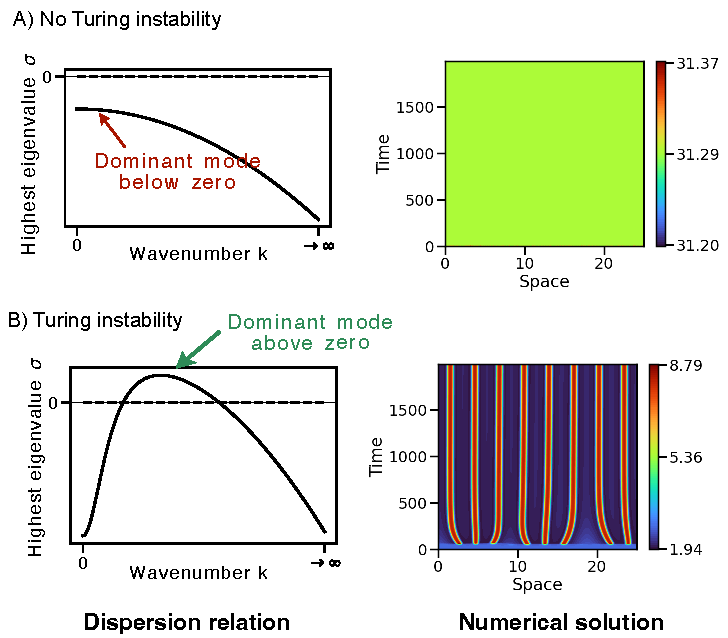
\includegraphics[width=1\textwidth]{chapters/Chapter 1/turing_vs_noturing} % The name of your image file; assumes it's in the same directory as your .tex file
    \caption[\textbf{The turing instability}]{\textbf{The turing instability}}
    \label{fig:turing_vs_noturing} % A label for referencing this figure later in the document
\end{figure}
An example of a classical turing instability with a positive dispersion peak is shown in Fig. \ref{fig:intro_to_turing_patterns}B, along with the corresponding stationary spatial pattern.
Alternatively,  Fig. \ref{fig:turing_vs_noturing}A shows a spatially homogeneous solution which results from a stable system that does not exhibit a diffusion driven instability.
These 1D numerical results were produced using the Crank-Nicholson numerical scheme described in ~\ref{cranknicolson}, which was I programmed from scratch in python. The boundary conditions used are Neumann boundary conditions where the derivative at the boundary is zero ($\pdv{U}{x}=0$) for both molecular species.

%todo add numbers to image
%todo add k and sigma
\subsection{Dataset creation}


\subsection{Infering wavelength and convergence time from dispersion relation}

Although the pattern cannot be observed using linear stability analysis, some information can be obtained from the dispersion relation.
Using the circuit defined in Eq. ~\eqref{eq:turinghill}, we simulated 500 parameter sets with a Turing instabilities as the one seen in Fig. \ref{fig:turing_vs_noturing}B. Then, the convergence time and wavelength for these patterns was measured using the algorithm described in %todo ref methods.
A linear relationship was found between the wavelength in the numerical pattern and the wavelength inferred from the dominant mode of the dispersion relation as seen in Fig. \ref{fig:dispersion_to_wavelength_convergence}A. However, the slope of the regression fitted to the data is smaller than 1, meaning the patterns obtained have a larger wavelength than the predicted linear stability analysis wavelength.
In terms of the convergence time, a non-linear correlation is observed between the highest eigenvalue $(\sigma)$ and the time for convergence.
Although some values do not correlate, we can overall state that systems with high eigenvalues generally converge faster than those lower eigenvalues Fig. \ref{fig:dispersion_to_wavelength_convergence}B.
These relationships are extremely important if we wish to understand characteristics of our system such as wavelength and convergence time without simulating the system numerically.
Specially if scanning through high dimensional spaces, such methods can be extremely informative to get an insight into patterns in this space.
Additionally, these relationships can be used prior to using numerical methods to choose relevant numerical parameters such as length of space and time of our simulation as well as dx and dt.



\begin{figure}[H] % h! is a placement specifier; it tries to place the image here.
    \centering
    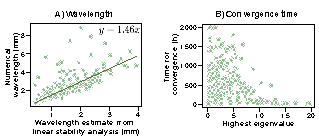
\includegraphics[width=1\textwidth]{chapters/Chapter 1/dispersion_to_wavelength_convergence} % The name of your image file; assumes it's in the same directory as your .tex file
    \caption{A sample caption for the image.}
    \label{fig:dispersion_to_wavelength_convergence} % A label for referencing this figure later in the document
\end{figure}

\subsection{Dispersion to pattern shape}
To further understand the information encoded in the dispersion relation, we focused on the dispersion height.
The approach used consisted in optimizing the dispersion peak height starting from an initial Turing pattern.
This way we can understand what happens to a specific pattern in parameter space when the dispersion peak height increases.
The optimization is carried out using a Markov-Chain Monte Carlo combined with the Metropolis algorithm, where the optimised function is the height of the dispersion peak (e.i the highest value of the highest eigenvalue) (See Methods). %TODO ref methods
The dispersion peak optimization path can be observed in Fig. \ref{fig:dispersion_peak_optimisation}A.
The resulting numerical patterns from the optimisation are then simulated and the convergence time measured as we did for Fig. \ref{fig:dispersion_to_wavelength_convergence}B. In Fig. \ref{fig:dispersion_peak_optimisation}B we can see a cleaner correlation of how the dispersion peak height determines the convergence time which could be modelled with an exponential decay function of the type
\begin{equation}
    f(x) = ae^{bx} + c
\end{equation}

This optimization was carried out for three different initial turing parameter sets. In Fig. \ref{fig:dispersion_peak_optimisation}C we can observe the pattern for the initial turing pattern and the turing pattern after optimization (with the highest dispersion peak).
While the with lower dispersion peaks present labyrinthian type of patterns, the patterns post-optimization present dot-like morphologies.
This suggests that a higher dispersion peak can lead to a preference for spots over labyrinths.


\begin{figure}[H] % h! is a placement specifier; it tries to place the image here.
    \centering
    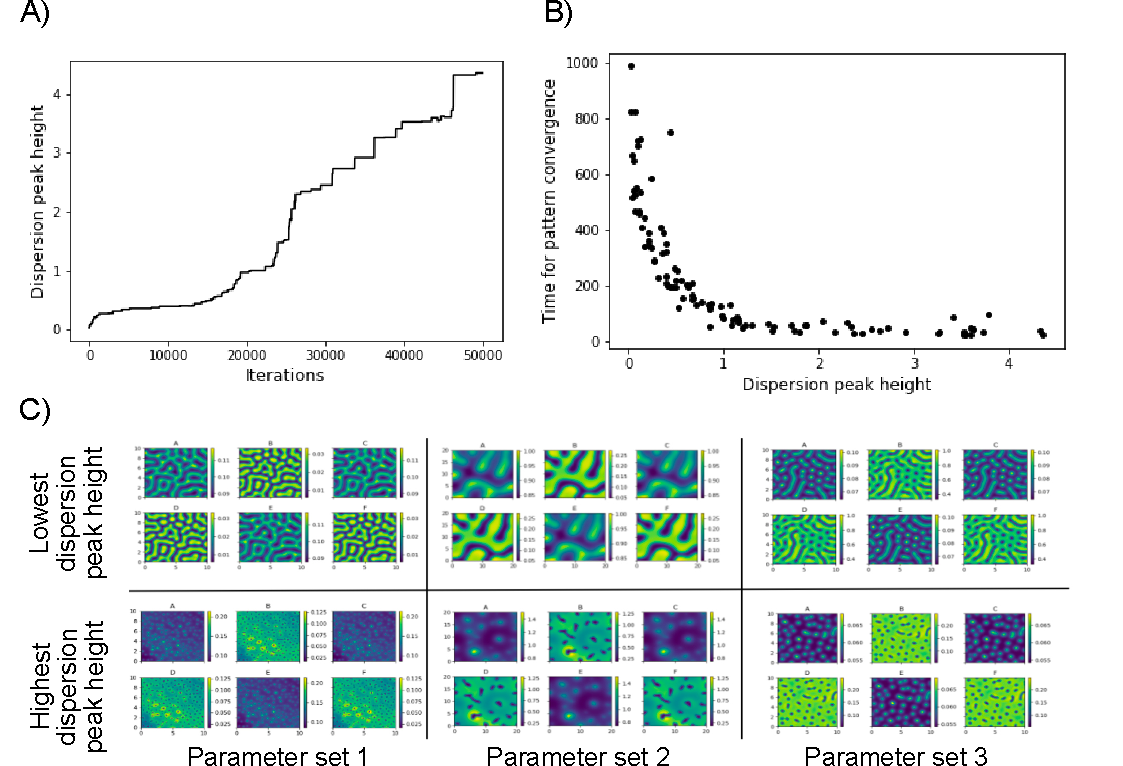
\includegraphics[width=1\textwidth]{chapters/Chapter 1/dispersion_peak_optimisation} % The name of your image file; assumes it's in the same directory as your .tex file
    \caption{A sample caption for the image.}
    \label{fig:dispersion_peak_optimisation} % A label for referencing this figure later in the document
\end{figure}



\section{Breaking linear stability analysis predictions}
Although Turing instabilities are a good indicator of patterned states, these instabilities are neither sufficient nor necessary for stationary periodic patterns to occur.
Current state-of-the-art literature analyses robustness for turing pattern formation using linear stability analysis to determine the Turing patterning parameter space.
With this type of analysis, you have a binary output which determines whether a parameter leads to a classical Turing instability or not as seen in Fig. \ref{fig:lsa_numerical_confusion_literature}.
However, the current assumptions in the TP literature, depicted by this confusion matrix shown in this figure, are a simplification of TPs prediction from linear stability analysis.
This is because the results from linear stability analysis give insights only into the local dynamics around a steady state.
Once the system moves away from the steady state and non-linearities are introduced, the system might behave differently and the local pattern dynamics might not be maintained.
For example, patterning instabilities that are not predicted by linear stability analysis might arise due to a subcritical bifurcations ~\parencite{villar, champneys}.
This is an example of a self-organising pattern where the classical Turing instability conditions are not necessary.


\begin{figure}[H] % h! is a placement specifier; it tries to place the image here.
    \centering
    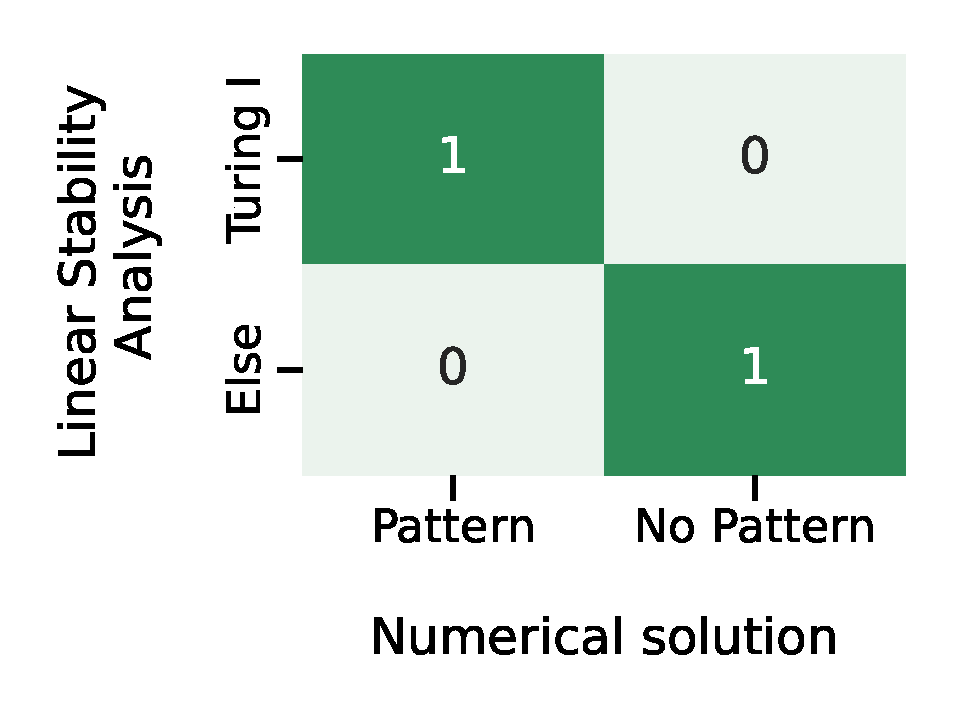
\includegraphics[width=0.6\textwidth]{chapters/Chapter 1/lsa_vs_numerical_confusion_literature} % The name of your image file; assumes it's in the same directory as your .tex file
    \caption{A sample caption for the image.}
    \label{fig:lsa_numerical_confusion_literature} % A label for referencing this figure later in the document
\end{figure}


\subsection{Multistability in Turing}
In this section, we demonstrate how linear-stability is not sufficient or necessary to predict TPs with multi-stable systems.
The motivation behind this arises from the high degree of multistability exhibited by biological systems, where cell-fate decisions have to be taken within this landscape. %TODO ref scholes thesis (37–40). %todo what leads to multistability? high number of nodes, high cooperativity?
Using the two-node non-linear Turing topology (Eq. \eqref{eq:turinghill}), multi-stable solutions were studied to understand how the patterning dynamics get affected when multiple steady state solutions are found.
First, linear stability analysis is carried out on a particular parameter sets to find multiple steady states of different stability nature (e.g. Stable, Unstable, Turing I, Turing I Hopf).
Then numerical simulations are computed where the initial condition is a random uniform distribution around a particular steady state.
Different pattern outcomes will result depending on where in the phase diagram the initial condition is.
Following the classical hypothesis used in the Turing robustness literature, we would expect Stable and Unstable systems to not produce patterns and Turing to produce patterns.
First, we present how this hypothesis can break under multistability conditions.
Fig. \ref{fig:multistability1} shows a case where diffusion-driven instability conditions are not required for TP formation.
The Unstable system, having a dispersion relation with a peak below zero, managed to get into a TP regime as it is attracted by the Turing equilibrium point.



\begin{figure}[H] % h! is a placement specifier; it tries to place the image here.
    \centering
    \begin{adjustbox}{center}
        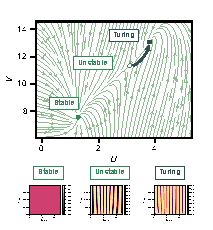
\includegraphics[width=1\textwidth]{chapters/Chapter 1/multistability1} % The name of your image file; assumes it's in the same directory as your .tex file
    \end{adjustbox}
    \caption{Turing pattern regimes attract neighbouring non-patterning equilibrium states.}
    \label{fig:multistability1} % A label for referencing this figure later in the document
\end{figure}

Then, we present a case where linear stability analysis cannot predict TP formation. Fig.~\ref{fig:multistability2} shows an ephemeral or transient pattern that occurs in the Unstable and Turing regimes.
The TP initially develops in the vicinity of the Turing steady state.
As the spatial heterogeneity is amplified and settles, it gets attracted by the stable steady state leading to the disruption of the pattern.
This type of transient pattern behaviour has also been recently reported in ~\cite{Krause2023}.

\begin{figure}[H] % h! is a placement specifier; it tries to place the image here.
    \centering
    \begin{adjustbox}{center}
        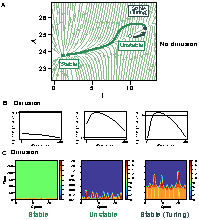
\includegraphics[width=1\textwidth]{chapters/Chapter 1/multistability2} % The name of your image file; assumes it's in the same directory as your .tex file
    \end{adjustbox}
    \caption{Ephemeral patterns}
    \label{fig:multistability2} % A label for referencing this figure later in the document
\end{figure}

Other examples can also be found, for example, where the unstable system settles into Turing, but the Turing system gets pulled by the Stable attractor (Fig.~\ref{fig:multistability_leftover}A). Additionally, some systems don't even exhibit a transient pattern and the three solutions are homogeneous in time and space (Fig.~\ref{fig:multistability_leftover}B). Finally, an unstable point might lie between to Turing points and therefore all three solutions will be a stationary periodic pattern (Fig.~\ref{fig:multistability_leftover}C).


\begin{figure}[H] % h! is a placement specifier; it tries to place the image here.
    \centering
    \begin{adjustbox}{center}
    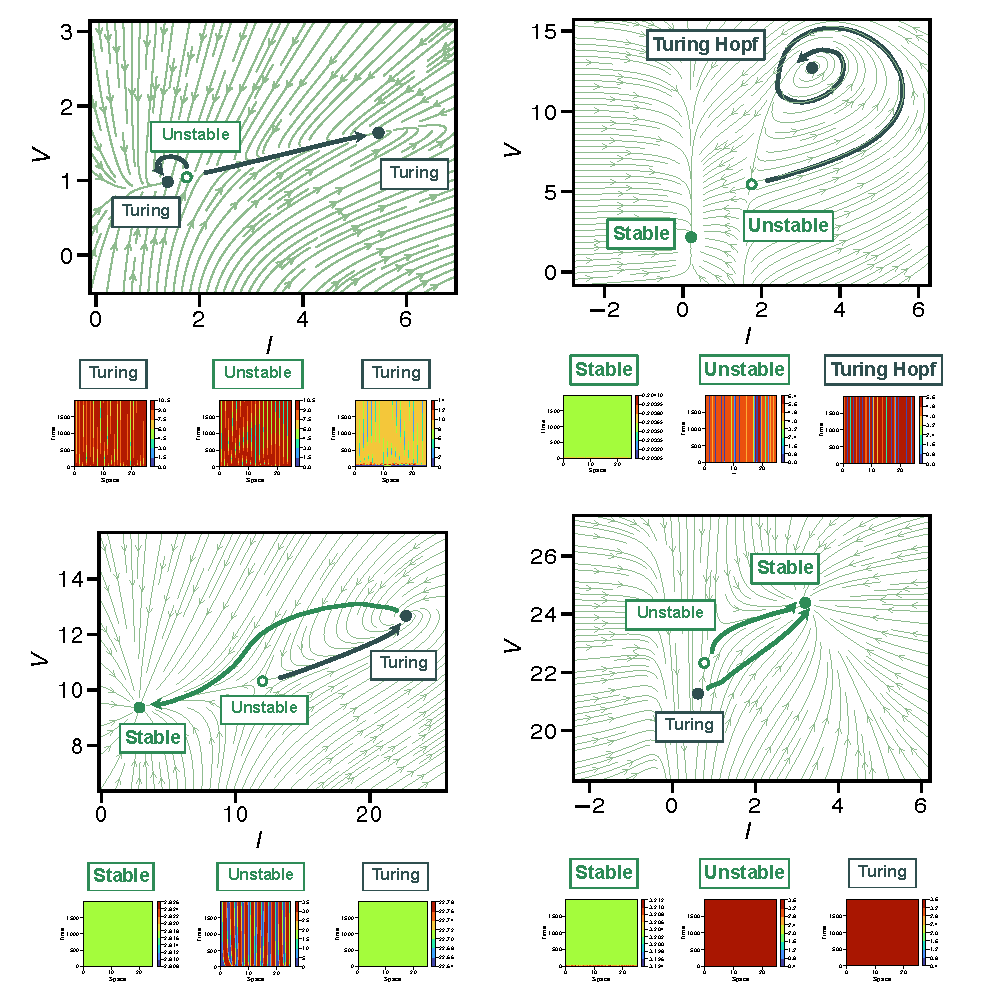
\includegraphics[width=1.4\textwidth]{chapters/Chapter 1/multistability_leftover} % The name of your image file; assumes it's in the same directory as your .tex file
    \end{adjustbox}
    \caption{Other types of multistability regimes.}
    \label{fig:multistability_leftover} % A label for referencing this figure later in the document
%TODO make subfigures bigger. Add letters to subfigures
\end{figure}


\subsection{Analytical to numerical: Other types of dispersion relation, and other types of patterns}
Multi-stable systems are not the only case where the classical turing instability fails to predict pattern formation.
Other types of dispersion relation beyond classical Turing instabilities can produce stationary patterns and non-stationary regular patterns that might be of interest in developmental biology.
The aim of this section is to document what type of dispersion relations in mono-stable systems can be linked to what type of patterns to gain insights into predicting pattern formation from linear stability analysis.
We will first present a classification for the different types of dispersion relation.
Then we will show the classification for the different types of pattern outcomes.
Finally, we will reconstruct the 2x2 confusion matrix (Fig. ~\ref{fig:lsa_numerical_confusion_literature}) currently used as an assumption in the literature for pattern formation to show a more complete understanding. The new confusion matrix will show more types of dispersion relation and more pattern outcomes with leading to a 5x4 confusion matrix.

First, we classify the outputs of dispersion relations from linear stability analysis into 5 types.
Stable dispersion relations have all eigenvalues $\sigma$ below zero for any wavenumber $k$, meaning there is no instability (Fig ~\ref{fig:dispersions}A).
Unstable dispersion relations have a positive eigenvalue at $k=0$ which eventually drops below zero as diffusion is introduced $k>0$ (Fig ~\ref{fig:dispersions}B).
As the unstable dispersion relation, the Hopf dispersion relation occurs when there is an instability without diffusion ($\sigma>0$ for $k=0$) which eventually drops below zero for positive wavenumbers.
However, in the case of Hopf dispersion relation, when the eigenvalues cross the zero line, there is a pair of complex conjugate eigenvalues (Fig ~\ref{fig:dispersions}C).
Turing I dispersion relations, as previously mentioned, are stable without diffusion and have an instability for a positive wavenumber and finally stable again for very large wavenumbers (Fig ~\ref{fig:dispersions}D).
Finally, Turing I hopf dispersion relations, are a combination of Turing I and Hopf dispersion relations.
As the Hopf bifurcation, they are unstable without diffusion.
Then, the stability kicks in with a pair of complex conjugates as the eigenvalues cross the zero line.
Finally, a Turing I type behaviour kicks in getting a peak above zero and decaying again for large wavenumbers (Fig ~\ref{fig:dispersions}E).
Other types of dispersion relation exist which are not displayed here such as Turing II, where the eigenvalues do not become stable again for very large wavenumbers.
Therefore, this system displays an instability at very large wavenumbers which result in infinitesimally small wavelength patterns.
These are considered to produce homogeneous solutions, except in the case of space discretization where they can produce small wavelength patterns ~\parencite{Wang2022}.
%TODO More detail on this classification can be found in methods x



%todo . They also identify examples of non-stationary spatial patterns, when the eigenvalue corresponding to a critical wave number has non-zero imaginary part.Deutsch, A., Dormann, S., et al., 2005. Cellular automaton modeling of biological pattern formation. Springer.

%todo look at pitchfork and transcritical

\begin{figure}[H] % h! is a placement specifier; it tries to place the image here.
    \centering
    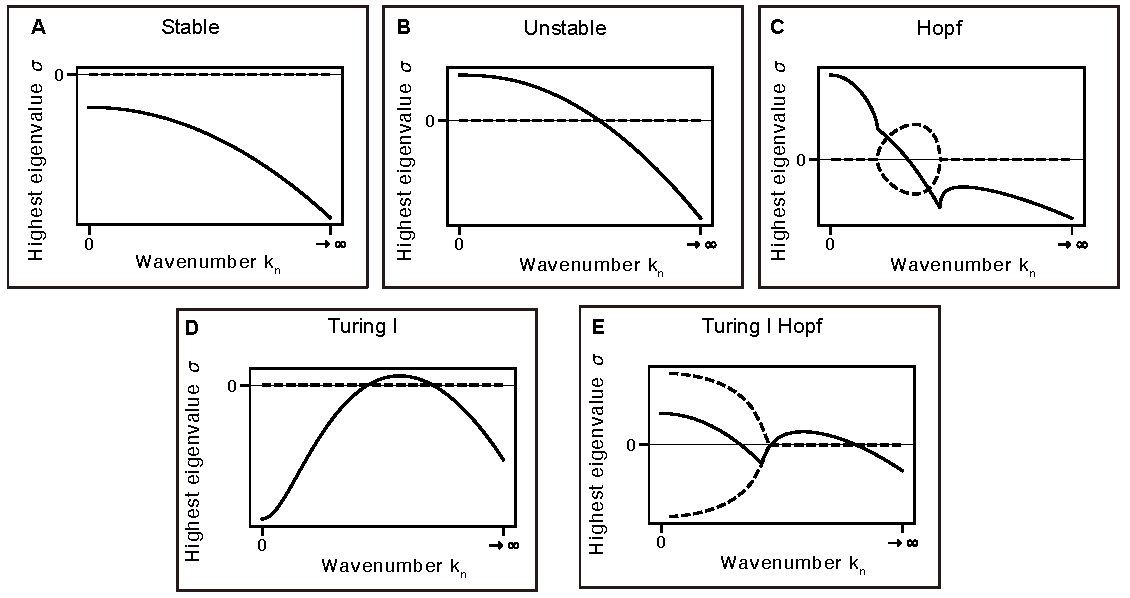
\includegraphics[width=1\textwidth]{chapters/Chapter 1/dispersions} % The name of your image file; assumes it's in the same directory as your .tex file
    \caption{A sample caption for the image.}
    \label{fig:dispersions} % A label for referencing this figure later in the document
\end{figure} %TODO add k and sigma to plots

We then need to classify the different types of patterns outcomes into 4.
We use a decision tree for the classification where the two layers are spatial homogeneity and convergence in time, as seen in Fig. ~\ref{fig:no growth classification}.
A pattern will be considered homogeneous if the final snapshot $U$ for any of the two molecular species fulfills the following condition
\begin{equation}
    \frac{max(U) - min(U)}{max(U)} \leq 0.01
\end{equation}
A pattern will be considered converged if the last 30 timepoints for any of the two molecular species fulfills the following condition
\begin{equation}
    \frac{max(U[-30:]) - min(U[-30:])}{max(U[-30:])} \leq 0.05
\end{equation}
The thresholds chosen were fine-tuned by testing them on the numerical patterns to obtain the best classification results.
Using this two characteristics, homogeneity and convergence, we can obtain 4 classes of patterns: Homogeneous, Temporal Oscillators, Non-stationary Patterns and Stationary Patterns (See Fig. ~\ref{fig:no growth classification}).
Homogeneous patterns are homogeneous in space and converge in time.
Temporal oscillators are homogeneous in space but do not converge, as they oscillate in time.
Non-stationary patterns are not homogeneous in space and do not converge in time.
Instead they show a spatial pattern that changes over time.
Finally, Stationary patterns are not homogeneous in pace but converge in time.


\begin{figure}[H] % h! is a placement specifier; it tries to place the image here.
    \centering
    \begin{adjustbox}{center}
    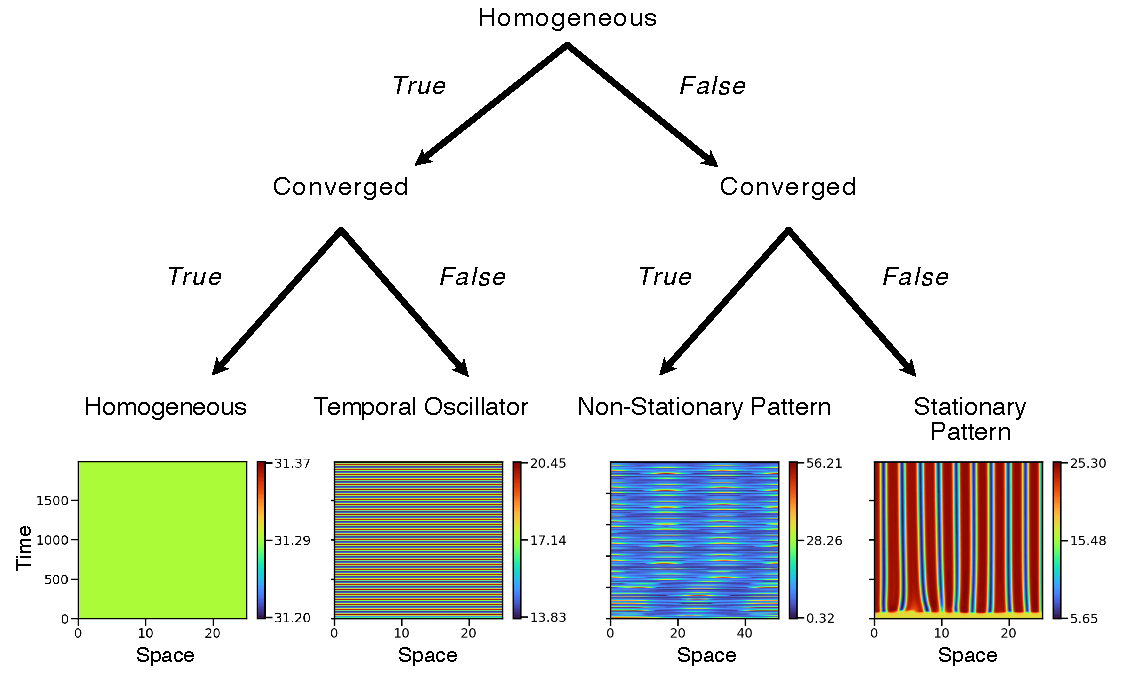
\includegraphics[width=1.2\textwidth]{chapters/Chapter 1/no growth classification} % The name of your image file; assumes it's in the same directory as your .tex file
    \end{adjustbox}
    \caption{Decision tree to classify patterns in non-growing domains}
    \label{fig:no growth classification} % A label for referencing this figure later in the document
\end{figure}


High throughput studies like ~\cite{Scholes2019, Zheng2016, Marcon} only consider Turing I as patterning and the rest is discarded.
Here, we explore beyond turing I and stationary patterns to give a more complete view of the relationship between linear stability and spatio-temporal patterns.
10000 parameter sets are analysed from the non-linear turing model (Eqs. \eqref{eq:turinghill}) to obtain dispersions relation numerical patterns.
Multi-stable systems are not included in this analysis to understand the direct relationships between the dispersion relation and numerics.
The two types of classifications describe above are applied, and a new 5x4 confusion matrix is generated (Fig. ~\ref{fig:lsa_numerical_confusion}).  %TODO check number of params

\begin{figure}[H] % h! is a placement specifier; it tries to place the image here.
    \centering
    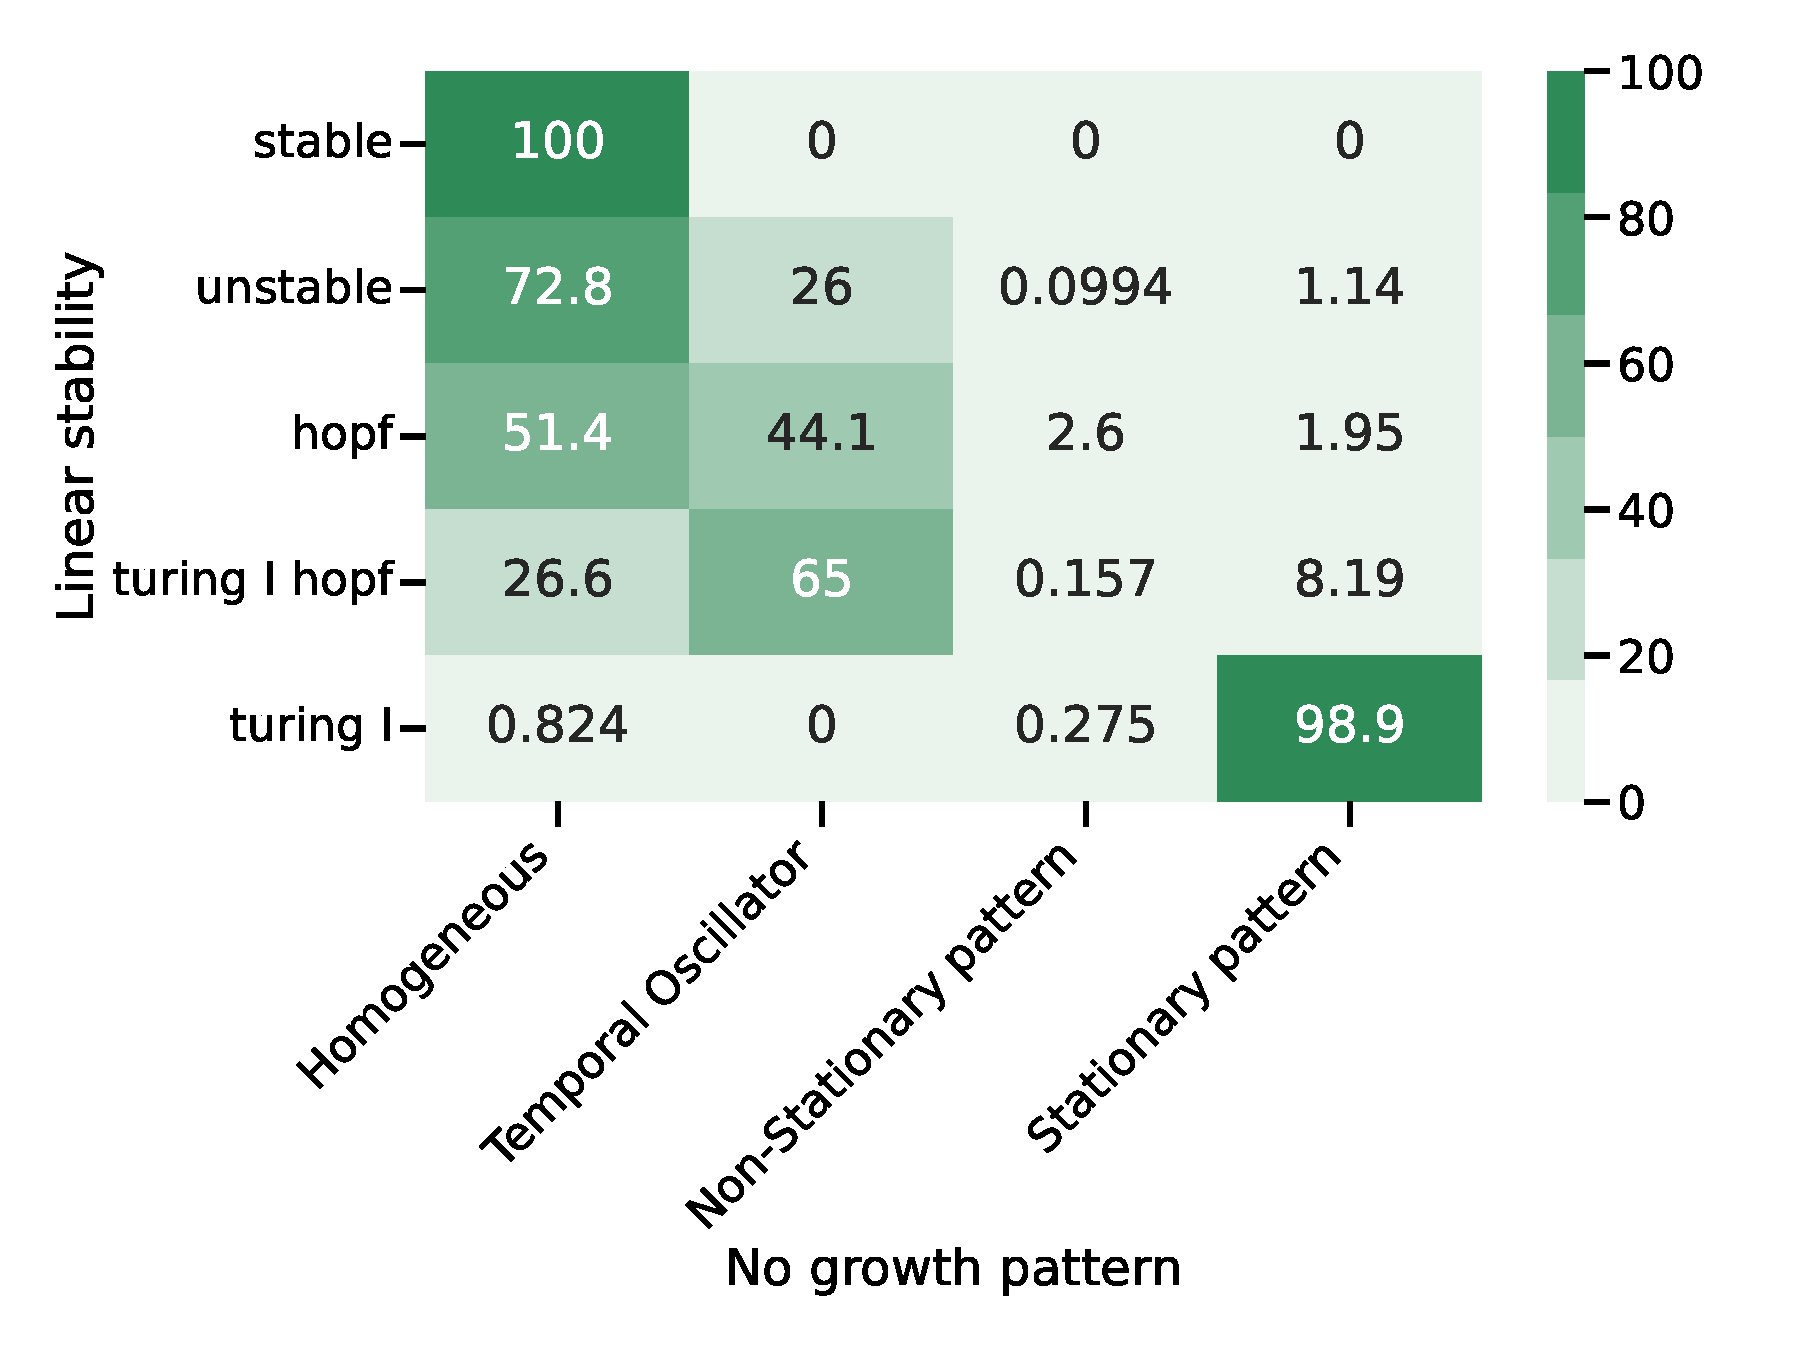
\includegraphics[width=1\textwidth]{chapters/Chapter 1/lsa_vs_numerical_confusion_variant0-11-12} % The name of your image file; assumes it's in the same directory as your .tex file
    \caption{\textbf{Confusion matrix to relate Linear stability Analysis output and numerical pattern outcome}}
    \label{fig:lsa_numerical_confusion} % A label for referencing this figure later in the document
\end{figure}

It is worth pointing out some interesting examples obtained from this confusion matrix.
For example, Turing I hopf seems to always lead to stationary patterns (See Fig. \ref{fig:interesting_cases_nogrowth}B), meaning they would definitely need to be included in high throughput robustness studies.
Some unstable dispersion relations lead to both stationary (See Fig. \ref{fig:interesting_cases_nogrowth}A) and non-stationary patterns.
Additionally, Hopf solutions also display interesting non-stationary patterns (See Fig. \ref{fig:interesting_cases_nogrowth}D).
Non-stationary patterns could also be of big interest in the field of developmental and synthetic biology as gene expression arrest could turn them into periodic stationary patterns.
Additionally, these non-stationary patterns could serve as a periodic pre-pattern for the initial symmetry breaking.
Unfortunately, some Hopf solutions are misclassified as Stationary patterns (See Fig. \ref{fig:interesting_cases_nogrowth}C) due to an inadequate threshold in the convergence classification.
It is important to understand that this is an initial exploratory analysis where classification might occur. This is because of the difficulty of common setting thresholds for a wide variety of numerica solutions with different wavelengths, time-scales and dynamic ranges.

\begin{figure}[H] % h! is a placement specifier; it tries to place the image here.
    \centering
    \begin{adjustbox}{center}
        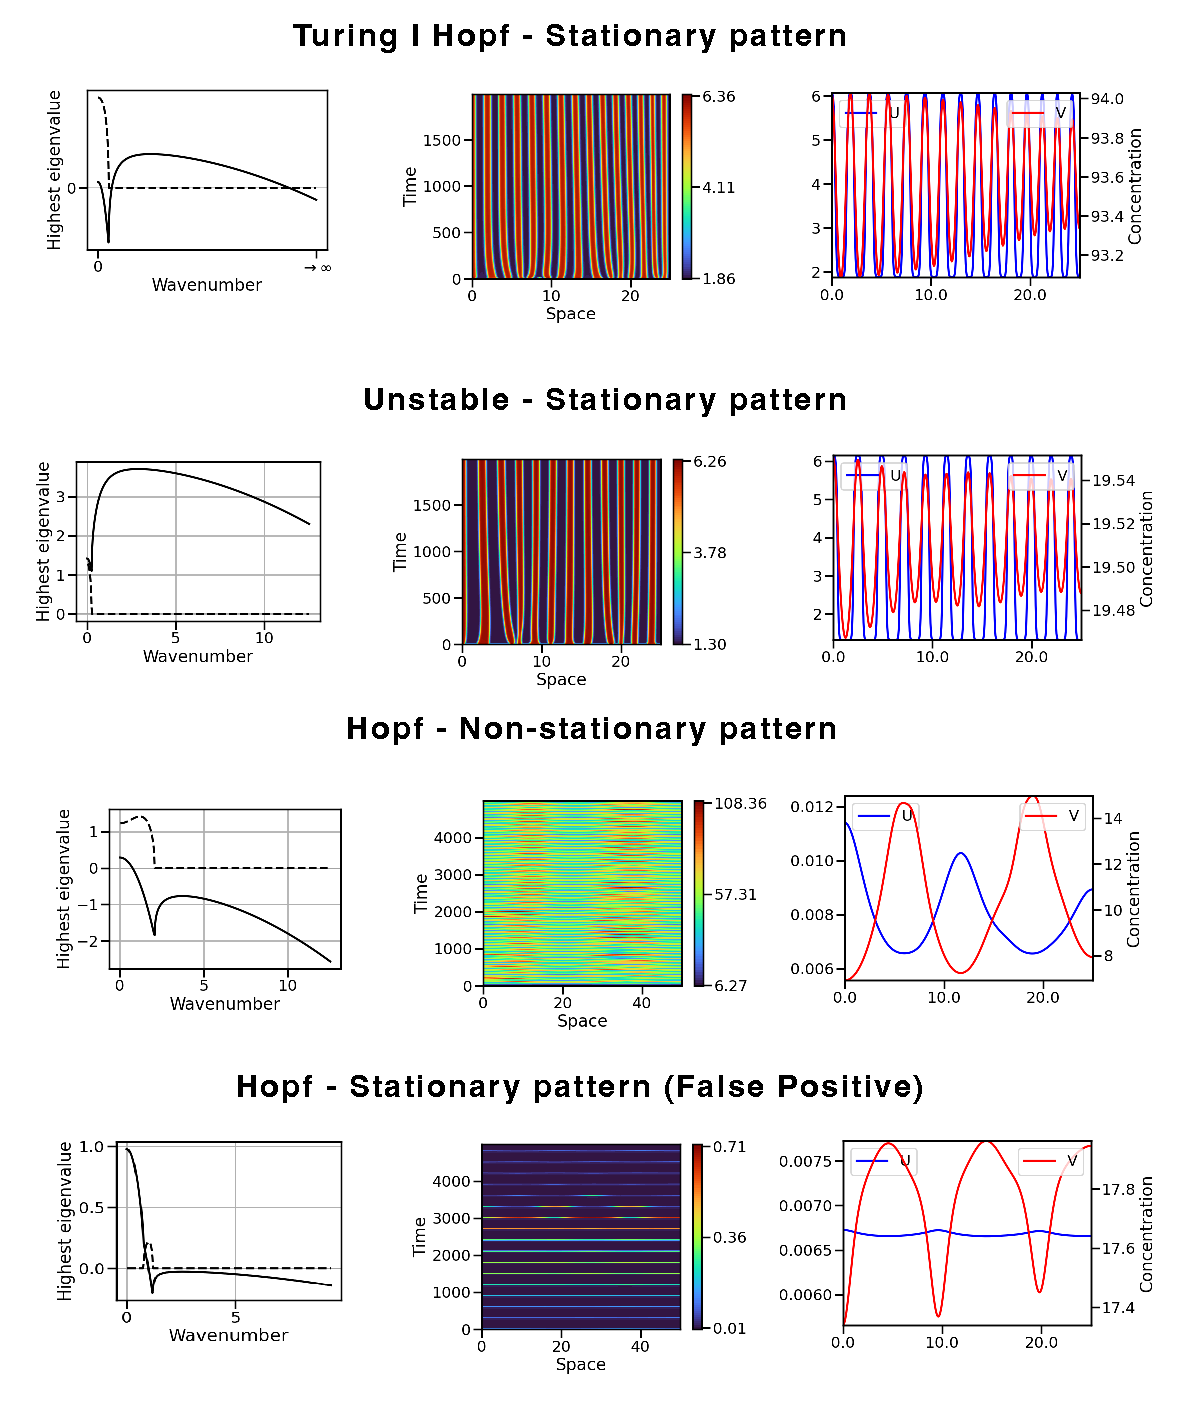
\includegraphics[width=1.2\textwidth]{chapters/Chapter 1/interesting_cases_nogrowth} % The name of your image file; assumes it's in the same directory as your .tex file
    \end{adjustbox}
    \caption{Interesting examples obtained from confusion matrix. }
    \label{fig:interesting_cases_nogrowth} % A label for referencing this figure later in the document
\end{figure}
\section{Introducing realistic biological phenomena}
As seen in the previous section both multistability effects and numerical solutions can break the hypothesis that only classical Turing I systems can produce stationary periodic patterns.
Here, we look deeper into how other aspects linking the theory closer to the biological reality can also break this hypothesis.
In particular, we will look at how adding an absorbing boundary condition and growth to the Turing problem might induce or break patterning.
This particular direction was inspired in experiments described in the next sections where growing bacterial colonies are used as a platform to engineer Turing patterns using synthetic gene circuits.

The absorbing boundaries are introduced by using a Dirilichet boundary condition where the concentration at the boundary is zero $u=0$ as opposed to the previously used Neumann boundaries where the derivative at the boundary is zero.
On the other hand, growth is introduced as isotropic linear growth, where cells are added to both boundaries with a linear growth rate.
Growth of the tissue is encoded in a 1D binary vector, where cells are denoted as 1 and empty space as 0.
The amount of 1's grows linearly, which represents the tissue expanding.
This vector is used as a mask, where 1's determine the computation of reaction-diffusion terms and 0's determine only the computation of diffusion.
Therefore, while reaction-diffusion occurs in the tissue; only diffusion occurs in the empty regions.

As with the non-growing Neumann boundary condition patterns in the previous section, we develop a classification system to quantify the different types of patterns obtained, and the transitions as growth is introduced.
However, due to the absorbing boundary conditions and growth homogeneity and convergence we previously defined is in some cases physically impossible.
For this reason, a new classification system is developed based on the number of peaks.
Peaks are detected using the python $find\_peaks$ algorithm with parameter
$prominence=0.05$.
Again, this can be tweeked depending on the numerical outcome and misclassification might occur.


\begin{figure}[H] % h! is a placement specifier; it tries to place the image here.
    \centering
    \begin{adjustbox}{center}
        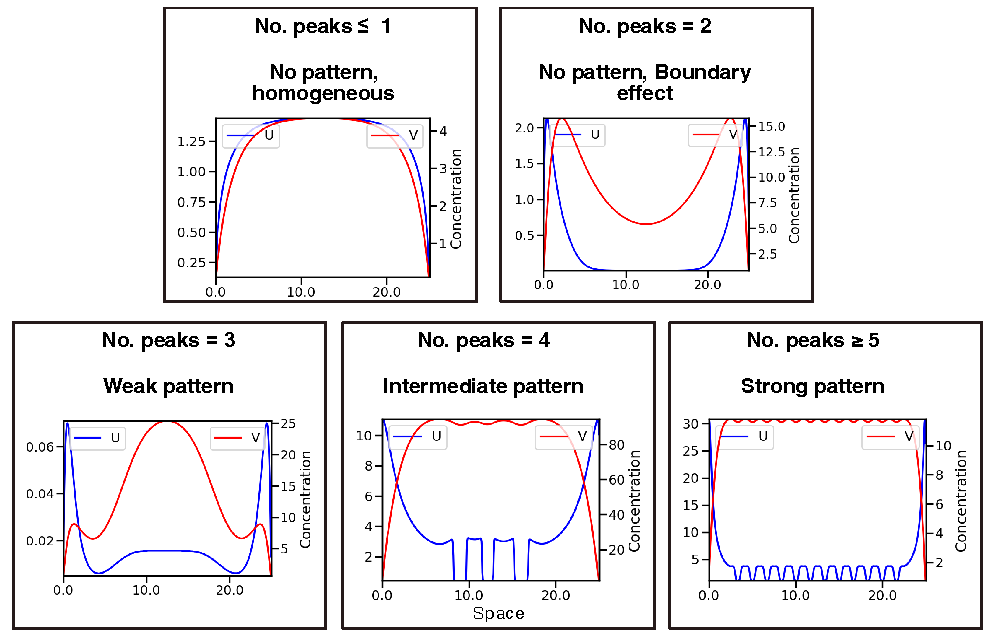
\includegraphics[width=1\textwidth]{chapters/Chapter 1/peaks_classification} % The name of your image file; assumes it's in the same directory as your .tex file
    \end{adjustbox}
    \caption{Classification based on peaks for absorbing boundary conditions and growth}
    \label{fig:peaks_classification} % A label for referencing this figure later in the document
\end{figure}

The peak classification shown in \ref{fig:peaks_classification}, retrieves information on whether there is a pattern at all and whether this pattern is only a pattern at the boundary or is a periodic pattern due to other effects.
Patterns with one 1 peak will be considered homogeneous as they result from the morphogens being reduced at the boundary due to absorption.
Patterns with 2 peaks are also considered not to be patterned states as the two peaks might arise at the boundary for one of the diffusers due to the depletion of the other.
Patterns with 3 peaks start displaying a more significant pattern, although it is hard to prove periodicity from them and the number of peaks might not scale with tissue length.
Patterns with 4 peaks could still be purely a boundary effect, but is less likely as periodicity starts being more present.
Finally, patterns with 5 peaks and above can be considered strong patterns and would be most similar to classical Turing patterns in non-growing no-flux boundary domains.


Using this classification method, x parameter sets where simulated and classified with absorbing boundary conditions and growth.
Again, all these parameter sets have only a single steady state to ensure patterning effects are due to boundaries and growth and not due to multistability.

%TODO make image on classification
%TODO add  2 confusion matrix


\subsection{No growth to open boundaries}

\begin{figure}[H] % h! is a placement specifier; it tries to place the image here.
    \centering
    \begin{adjustbox}{center}
        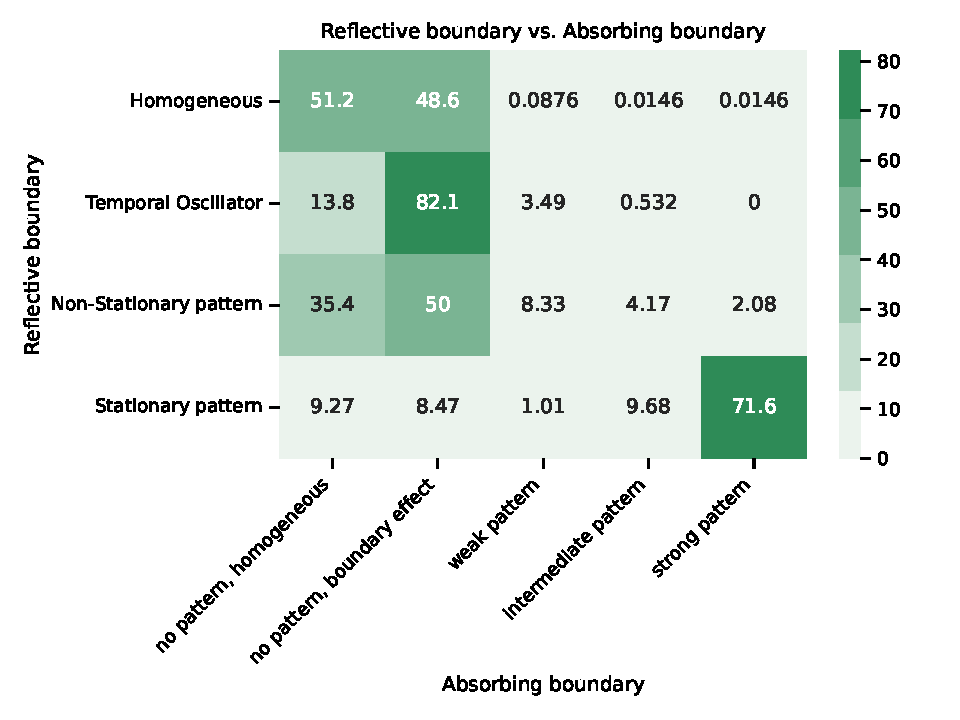
\includegraphics[width=1\textwidth]{chapters/Chapter 1/nogrowth_openboundary_confusion_variant0-11-12} % The name of your image file; assumes it's in the same directory as your .tex file
    \end{adjustbox}
    \caption{Effects of absorbing boundary conditions on patterning}
    \label{fig:nogrowth_openboundary_confusion_variant0} % A label for referencing this figure later in the document
\end{figure}


\begin{figure}[H] % h! is a placement specifier; it tries to place the image here.
    \centering
    \begin{adjustbox}{center}
        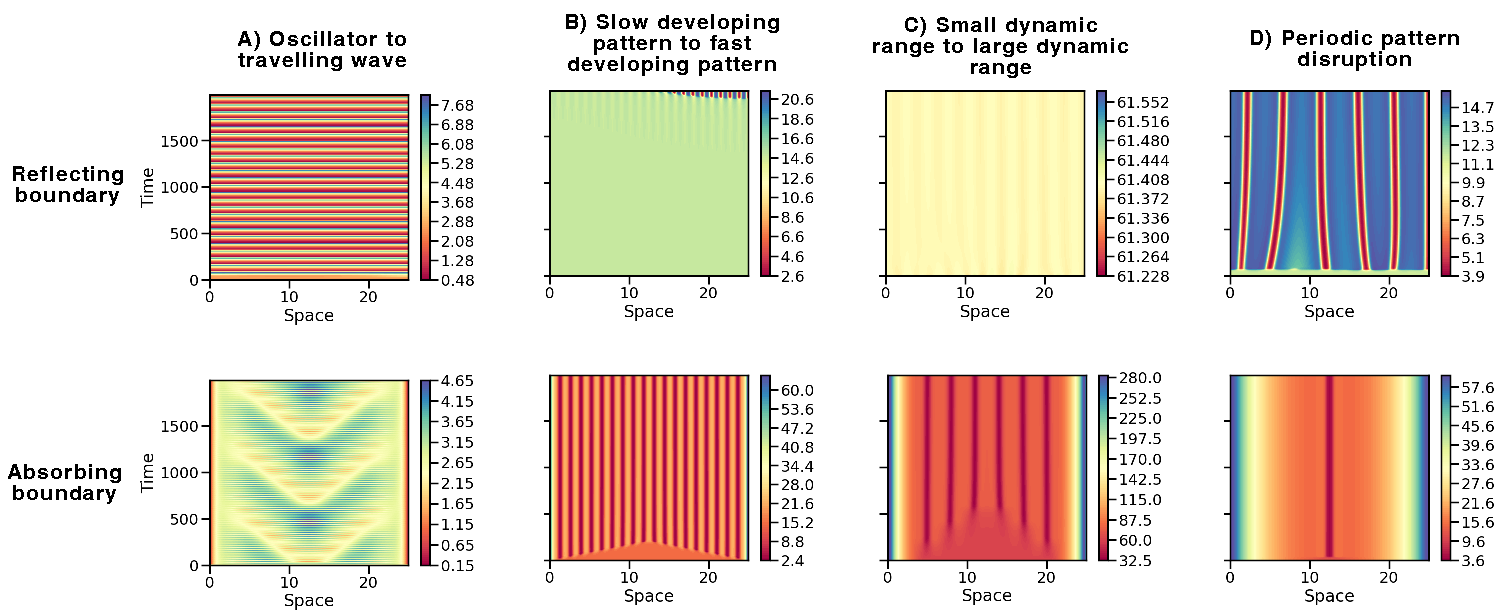
\includegraphics[width=1\textwidth]{chapters/Chapter 1/interesting_cases_openboundary} % The name of your image file; assumes it's in the same directory as your .tex file
    \end{adjustbox}
    \caption{Interesting cases when boundary is added}
    \label{fig:interesting_cases_openboundary} % A label for referencing this figure later in the document
\end{figure}


\subsection{Open boundaries to growth}

\begin{figure}[H] % h! is a placement specifier; it tries to place the image here.
    \centering
    \begin{adjustbox}{center}
        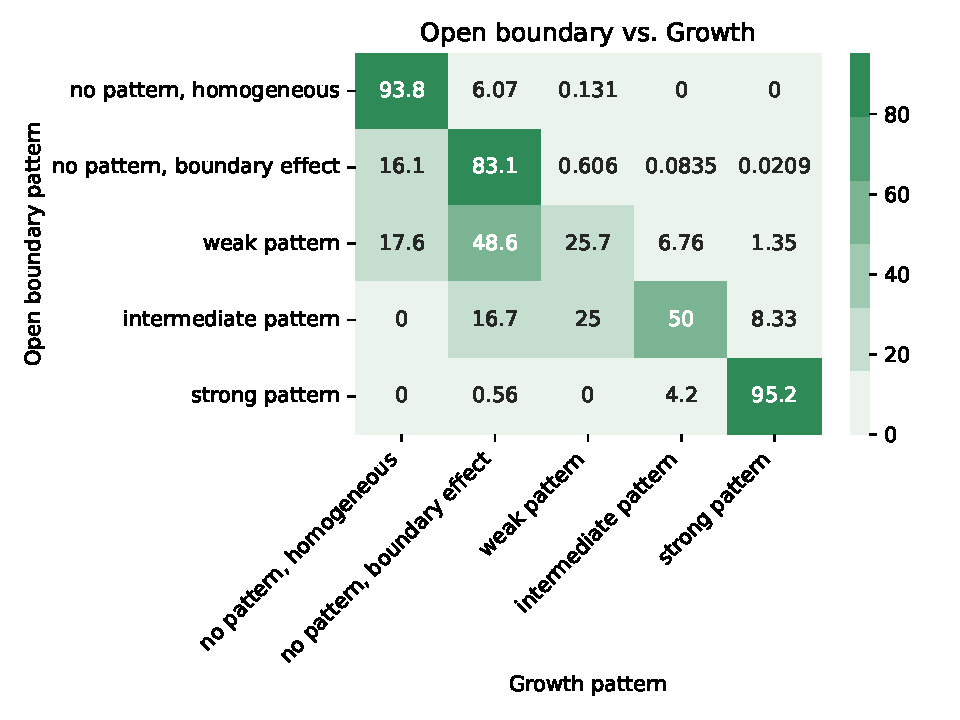
\includegraphics[width=1\textwidth]{chapters/Chapter 1/openboundary_edgegrowth2_confusion_variant0-11-12} % The name of your image file; assumes it's in the same directory as your .tex file
    \end{adjustbox}
    \caption{Classification based on peaks for absorbing boundary conditions and growth}
    \label{fig:openboundary_edgegrowth2_confusion_variant0} % A label for referencing this figure later in the document
\end{figure}


\begin{figure}[H] % h! is a placement specifier; it tries to place the image here.
    \centering
    \begin{adjustbox}{center}
        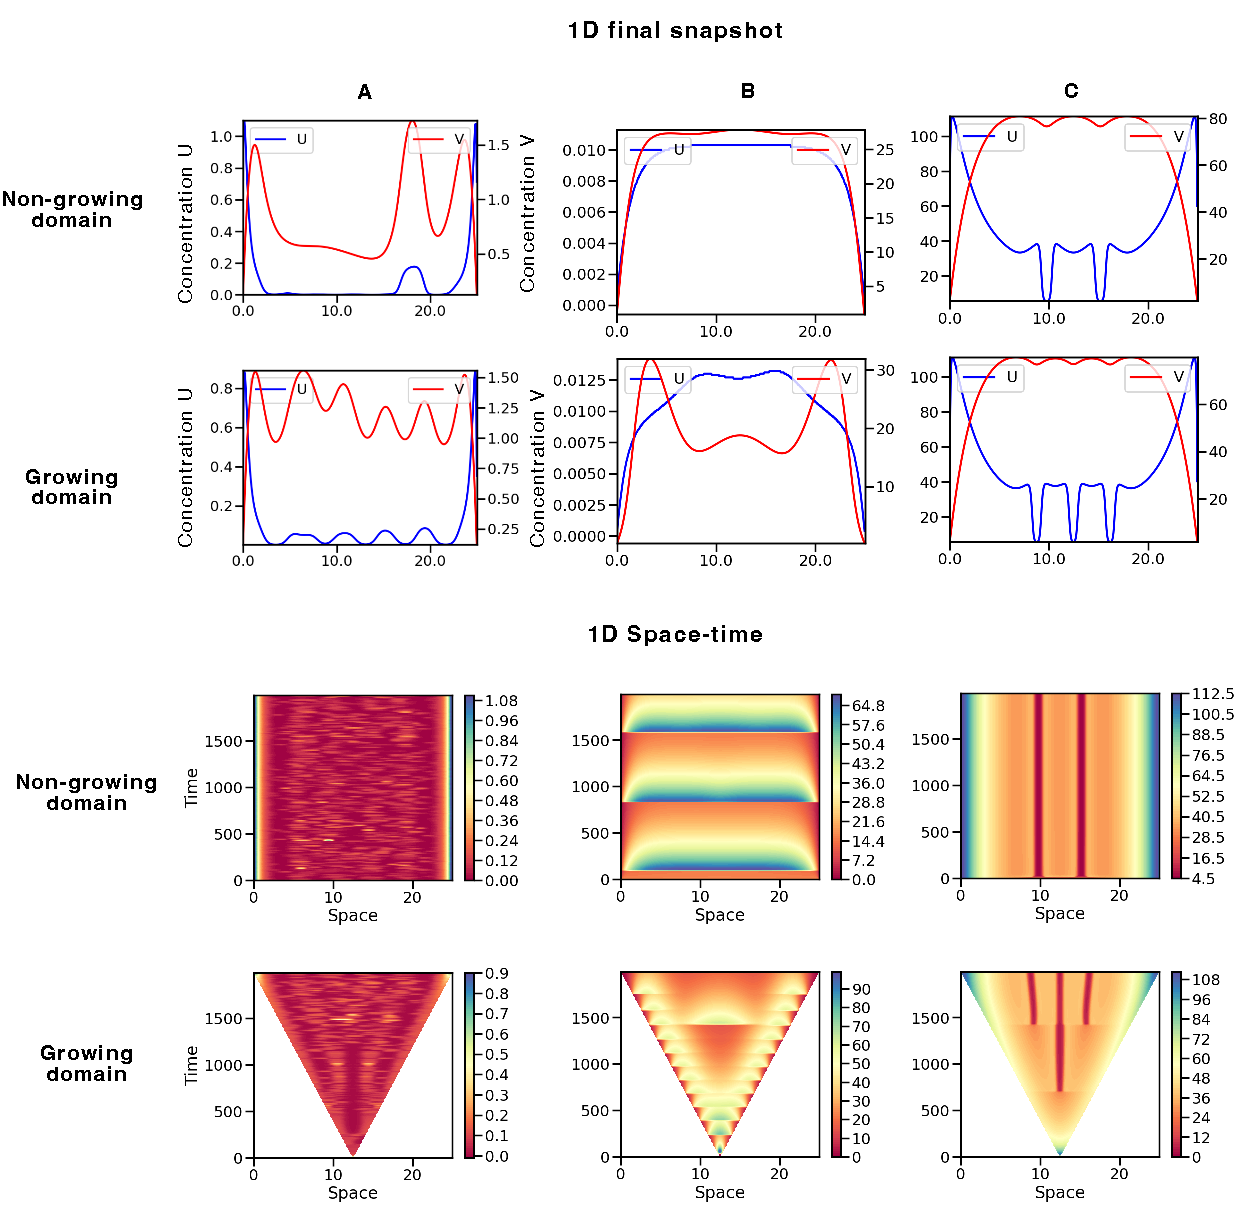
\includegraphics[width=1\textwidth]{chapters/Chapter 1/interesting_cases_edgegrowth2} % The name of your image file; assumes it's in the same directory as your .tex file
    \end{adjustbox}
    \caption{Classification based on peaks for absorbing boundary conditions and growth}
    \label{fig:interesting_cases_edgegrowth2} % A label for referencing this figure later in the document
\end{figure}




\begin{figure}[H] % h! is a placement specifier; it tries to place the image here.
    \centering
    \begin{adjustbox}{center}
        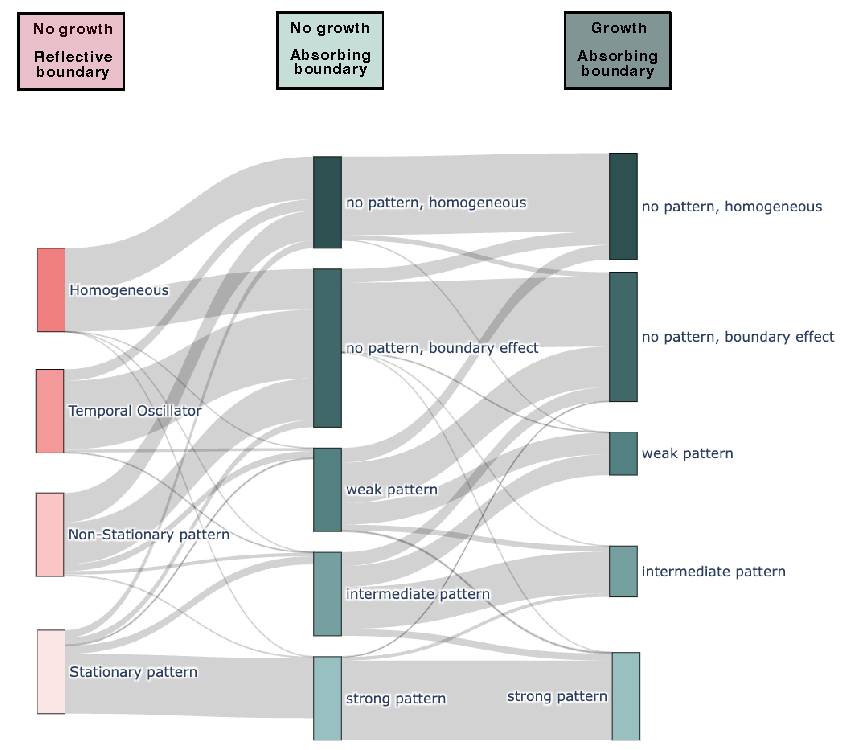
\includegraphics[width=1\textwidth]{chapters/Chapter 1/3layer_sankey} % The name of your image file; assumes it's in the same directory as your .tex file
    \end{adjustbox}
    \caption{Classification based on peaks for absorbing boundary conditions and growth}
    \label{fig:3layer_sankey} % A label for referencing this figure later in the document
\end{figure}








    % Chapter Template
\chapter{Gene circuit definition, exploration and parametrisation} \label{chapter2}
Up to now, Turing circuits that give rise to regular patterns, have only been engineered in chemical systems.
Using synthetic biology, we aimed to engineer Turing patterns in biological systems using gene circuits that exhibit reaction-diffusion (RD).
An RD synthetic gene circuit was built in~\cite{Tica2020}
using gene regulatory functions and quorum sensing components.
The reaction term comes from activation or inhibition by proteins binding to promoter or operator regions upstream of a gene
and regulating its expression.
The diffusion term describes the quorum-sensing molecules acting as morphogens and diffusing across the tissue,
as well as forming complexes with receptors to regulate gene expression.
Transitioning from a synthetic RD circuit to the generation of Turing patterns is not a trivial task due to the lack of parametric robustness of Turing systems.
To address this complex task, a model is needed which can help us understand the dynamic behaviour of the RD gene circuit and whether it can produce patterns.
Additionally, because of the lack of parametric robustness, it is important to learn how to tune parameters to increase the probability of obtaining patterns.

In this chapter, we present a model which describes this gene circuit.
Additionally, we explore the parameter space based on literature-informed ranges to understand what fraction of it leads to Turing and how to tune the circuit to obtain a higher probability of patterning.
Finally, to obtain a model which is more closely linked to our experimental system and yields more accurate predictions,
we parametrise it using liquid culture data.

Work in this chapter and the following Chapter~\ref{chapter3} has been published as a preprint in~\cite{Oliver2023}.
\section{Building model describing synthetic gene circuit}
In this section, I present a model which describes the synthetic gene circuit engineered in~\cite{Tica2020}.
The circuit can be seen in Fig.~\ref{fig:synthetic circuit_chapter2}, which was already presented in Chapter~\ref{introduction} but is repeated here to facilitate access to the reader.

\begin{figure}[H]
    \centering
    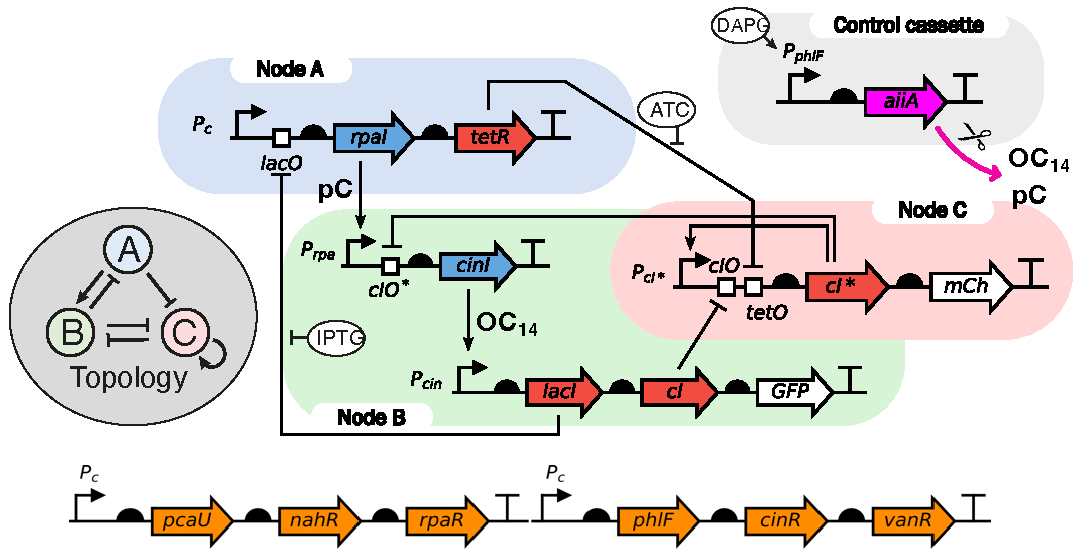
\includegraphics[width=1\textwidth]{chapters/Chapter 2/synthetic circuit2}
    \caption{\textbf{Synthetic biology implementation of \#1754 topology.} This synthetic circuit
    engineered by Dr.~Jure Tica and Tong Zhu is a genetic abstraction of the \#1754 topology in \cite{Scholes2019}.
    This circuit is transformed so every \textit{E.~coli} cell in the biofilm has a copy inside.
    The original topology (left, grey inset) has only three nodes, while the synthetic circuit (right) has six nodes.
    The six-gene circuit architecture, shown in standard notation, can be clustered into the three original nodes
    as seen by the blue, green and red bubbles.
    Diffusor synthesis enzymes, in blue, produce quorum sensing molecules $pC$ and $OC_{14}$ which diffuse out of the cell (blue and green arrows).
    Non-diffusible transcription
    factors (in red), also called repressor proteins, are lacI, cI, cI* and tetR.
    Fluorescent proteins GFP and mCherry are in white.
    The circuit can be regulated by small molecules aTc, IPTG and DAPG shown in white bubbles.
    DAPG activates the control cassette and produces regulated degradation of small quorum sensing molecules.
    The bottom cassette (orange), contains the necessary regulators:
    rpaR is the pC receptor (Node A diffusor), cinR is the OC14 receptor (Node B diffusor),
        and phlF is the DAPG receptor (used to tune inducible diffusor degradation).}
    \label{fig:synthetic circuit_chapter2}
\end{figure}

A \acrfull{PDE} system is used to describe the reaction and diffusion terms of this synthetic gene circuit (Fig.~\ref{fig:synthetic circuit_chapter2}).
This system of equations describes the concentration of molecules which are the dependent variables, in time and space which are the independent variables.
The molecules modelled are the six regulator genes and two diffusor molecules.
Diffusor molecules act as morphogens in this RD circuit.
This model includes:
\begin{itemize}
    \item Constant background production due to promoter leakiness
    \item Activator-repressor regulated gene expression using non-linear sigmoidal Hill terms
    \item Linear degradation of proteins and diffusor molecules or morphogens
    \item Diffusion of morphogens in a ~\acrfull{2D} space
    \item Effect of tuning molecules aTc, IPTG and DAPG on the circuit and diffusion
    \end{itemize}
The dynamics of a generic protein (X) and generic morphogen  (U) of the gene circuit, which are regulated by the activator [A] and inhibitor [I], are modelled in 2D as

\begin{subequations}\label{eq:Generalised protein and diffuser pde}
\begin{equation}
    \pdv{[X]}{t}= b_{X}+V_{X}\cdot\frac{1}{1+\left(\frac{K{A}}{[A]}\right)^{n_{A}}}\cdot\frac{1}{1+\left(\frac{[I]}{K_{I}}\right)^{n_{I}}}-\mu_{X}\cdot[X]
    \label{eq:Generalised protein}
\end{equation}

\begin{equation}
    \pdv{[U]}{t} = k_{1}\cdot[A] - \mu_{U}\cdot[U] + D_{U}\nabla^2 [U]
    \label{eq:generalised diffuser}
\end{equation}
\end{subequations}

This results in a PDE model with eight equations that correspond to the two diffusors
(pC and OC14) and six protein species of the circuit:
RpaI, CinI, TetR, LacI, cI* and cI.
This PDE model is reduced to a six-equation system by assuming a quasi-steady state for the diffusors,
with production and degradation kinetics much faster than those of proteins.
Finally, the model is non-dimensionalised to enable its parametrisation using liquid culture dose-response data.
This non-dimensionalisation involves tranaforming the model so the variables are expressed in terms of dimensionless units instead of concentration units.
In the subsections below, the different terms of Eq.~\ref{eq:Generalised protein and diffuser pde} are discussed.
Furthermore, the process of model reduction, non-dimensionalisation and fitting is also described.


\subsection{Protein equations and gene regulation}\label{Protein equations and gene regulation}
The rate of protein production can be defined as
\begin{equation}
    V = V_{max} \cdot \theta([X])
    \label{eq: vmax}
\end{equation}
where $\theta$ is a function of a generic protein X concentration which represents the fractional activation of the system.
Full activation of protein production is denoted as $\theta=1$ while full inhibition is represented by $\theta=0$.
$V_{\max}$ is the maximal rate of expression.
$\theta$ can be represented by a Hill function and an inverse-Hill function to describe cooperative binding,
derived using the law of mass action with all-or-none binding to multiple binding sites ~\parencite{Weiss1997}.
We further apply the quasi-steady state assumptions for activator and inhibitor binding to the promoter,
as well as for the mRNA dynamics,
as these timescales are much faster than protein production ~\parencite{Andersen1998, Bremer2008}.
This leads to the following expression of $\theta$ for non-competitive activation (A) and inhibition (I)
\begin{equation}
    \theta([A],[I])= \frac{1}{1+\left(\frac{K_{A}}{[A]}\right)^{n_{A}}} \cdot \frac{1}{1+\left(\frac{[I]}{K_{I}}\right)^{n_{I}}}
    \label{eq:theta}
\end{equation}
This Hill function is used in the Eq.~\ref{eq:Generalised protein} and describes promoter activity as a function of the two inputs [A] and [I], where $K_{A}$ and $K_{I}$ are half-activation/inhibition concentrations, $n_{A}$ and $n_{I}$ are the Hill coefficients.
Additionally, most promoters are leaky,
which we account for by introducing a small rate of background production $b_{X}$.
corresponds to the first term in Eq.~\ref{eq:Generalised protein}

\begin{figure}[H] % h! is a placement specifier; it tries to place the image here.
    \centering
    \begin{adjustbox}{center}
        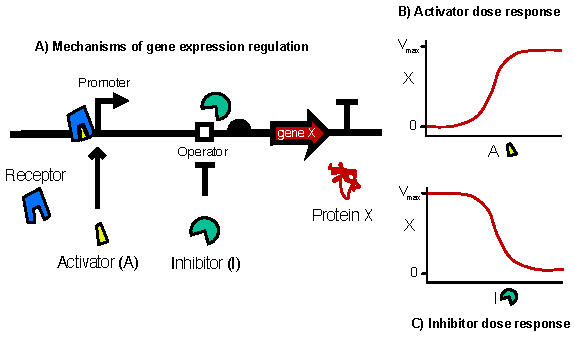
\includegraphics[width=1\textwidth]{chapters/Chapter 2/activation_inhibition2} % The name of your image file; assumes it is in the same directory as your .tex file
    \end{adjustbox}
    \caption{\textbf{Activation and Inhibition of gene expression.} \textbf{(A)} Mechanisms of gene expression regulation:
    The activator molecule (yellow) binds a receptor (blue),
        and this complex binds the promoter to activate gene expression.
    The inhibitor (green) binds the operator and inhibits gene expression.
    In the case of this model, activators are diffusors (pC, $OC_{14}$) with their respective receptors (RpaR, CinR) and inhibitors are proteins (RpaI, CinI, TetR, LacI, cI, cI*).
    \textbf{(B)} Expression of X dependent on activation by A modelled with a Hill function.
    \textbf{(C)} Expression of X dependent on inhibition by I modelled with an inverse-Hill function.}
    \label{fig:activation_inhibition} % A label for referencing this figure later in the document
\end{figure}

A visual representation of the mechanisms of activation and inhibition
modelled in Eq.~\ref{eq:theta} can be observed in Fig.~\ref{fig:activation_inhibition}.
Using Eq.~\ref{eq: vmax} and Eq.~\ref{eq:theta}, activator and inhibitor dose curves are be generated
(Fig.~\ref{fig:activation_inhibition}B-C).
These dose-response curves show the relationship between the activator or inhibitor and the rate of production of protein X.
Steeper curves are generated with higher cooperativity constants,
which are typical of cooperative systems where multiple transcription factors (TFs) can bind simultaneously.
These steep curves resemble electrical engineering circuits,
which use step functions instead of dose-response curves,
meaning a specific inducer concentration will drive the system from 0 to $V_{\max}$.
Finally,
the K parameter in Eq.~\ref{eq:theta} corresponds to the concentration of inducer
required to reach production of X at  $1/2 V_{\max}$.


\subsection{Tuning gene expression: aTc regulation of TetR and IPTG regulation of LacI}
Experimentally, the circuit was designed to be tuned in a variety of ways using aTc, IPTG and DAPG.
This tuning was used to achieve parameter combinations that are more favourable for patterning.
The following section introduces aTc and IPTG tuning into the model.

\begin{figure}[H] % h! is a placement specifier; it tries to place the image here.
    \centering
    \begin{adjustbox}{center}
        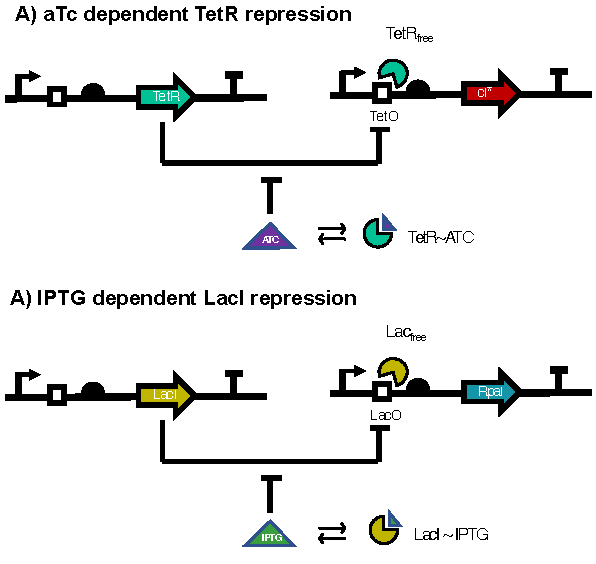
\includegraphics[width=0.7\textwidth]{chapters/Chapter 2/inducers} % The name of your image file; assumes it is in the same directory as your .tex file
    \end{adjustbox}
    \caption{\textbf{aTc and IPTG dependent repressions.}
    \textbf{(A)} TetR represses cI* by binding the TetO operator sequence.
    This repression can be inhibited by competitive binding of aTc to TetR.
    \textbf{(B)} LacI repression of RpaI* is inhibited by IPTG through competitive binding to LacI.}
    \label{fig:inducers} % A label for referencing this figure later in the document
\end{figure}

As shown in Fig.~\ref{fig:inducers}A, aTc binds to TetR and inactivates it.
Only free, unbound TetR can bind TetO and inactivate the expression of cI*.
The binding of aTc to TetR is modelled by a reversible equilibrium.
The affinity of binding is given by the $k_{on}$ and $k_{off}$ rate constants.

\begin{equation}
    aTc + TetR_{free} \xrightleftharpoons[k_{off}]{k_{on}} TetR \mhyphen aTc
\end{equation}

The law off mass action where the rate of reaction is the rate
constant multiplied by the concentration of reactants is applied.
Additionally, because this equilibrium happens at much faster rates than the protein production and degradation reactions of the model.
For this reason, quasi-steady state, which is valid when the system reaches equilibrium, is assumed

\begin{equation}
    \pdv{TetR \mhyphen aTc}{t} = k_{on}[TetR_{free}][aTc]^{n_{aTc}} - k_{off}[TetR \mhyphen aTc] \approx 0
\end{equation}


By rearranging terms and using $K_{D} = k_{off}/k_{on}$, a simplified expression for $[TetR_{free}]$ is obtained,
which is then used in the model

\begin{equation}
[TetR_{free}] = K_{D}\cdot \frac{[TetR \mhyphen naTc]}{[aTc]^{n_{aTc}}}
\end{equation}

Considering TetR is either free or bound to aTc, $[TetR-naTc]$ can be expressed as

\begin{equation}
[TetR \mhyphen naTc] = [TetR_{total}] - [TetR_{free}]
\end{equation}

to obtain the following expression

\begin{subequations}
    \begin{equation}
    [TetR_{free}] = K_{D} \cdot \frac{[TetR_{total}] - [TetR_{free}]}{[aTc]^{n_{aTc}}} \Longrightarrow
    \end{equation}
    \begin{equation}
    [TetR_{free}] (1+\frac{K_{D}}{[aTc]^{n_{aTc}}}) = \frac{K_{D}\cdot [TetR_{total}]}{[aTc]^{n_{aTc}}}\Longrightarrow
    \end{equation}
    \begin{equation}
    [TetR_{free}] = \frac{K_{D}\cdot[TetR_{total}]}{[aTc]^{n_{aTc}}+K_{D}} = \frac{[TetR_{total}]}{1+\frac{[aTc]^{n_{aTc}}}{K_{D}}}
    \end{equation}
\end{subequations}

which says that the concentration of unbound TetR is given by ~$[aTc]$,
~$[TetR_{total}]$ and the equilibrium constant ~$K_{D}$.

For non-cooperative systems where ~$n=1$, ~$K_{D}=[L_{half}]$, where $[L_{half}]$ is the $[aTc]$ at half repression.
However, for cooperative systems where ~$n>1$, ~$[L_{half}] = \sqrt[n]{K_{D}}$.
We define a new variable ~$K_{A} = \sqrt[n]{K_{D}} \leftrightarrow K_{D} = K^n_{A}$
that we use to replace ~$K_{D}$ in the following expression,
where $K^n_{A}$ is written as $K_{TetR \mhyphen aTc}$.
This was also done for other ~$K_{D}$ parameters of the model.
\begin{equation}
[TetR_{free}] =  \frac{[TetR_{total}]}{1+(\frac{[aTc]}{K_{TetR \mhyphen aTc}})^{n_{aTc}}}
\end{equation}
Parameter $K_{TetR \mhyphen aTc}$ is the dissociation constant of aTc to TetR,
whereas $n_{aTc}$ is the cooperativity of TetR and aTc binding.
This expression for unbound TetR ($[TetR_{free}]$ ), can then be introduced into the production rate of cI*.
cI* has an operator sequence downstream of the promoter, TetO.
This TetO is bound by TetR to inhibit the expression of the mRNA.
We will model the production of cI* dependent on TetR binding,
using an inverse-Hill term
that describes repression by this binding as described by Eq.~\ref{eq: vmax} and Eq.~\ref{eq:theta}.

\begin{equation}
    \pdv{[cI*]}{t} = V_{max}\cdot \left(1+\left(\frac{[TetR_{free}]}{K_{TetR \mhyphen TetO}}\right)^{n_{TetO}}\right)^{-1} = V_{max} \cdot \left(1+\left(\frac{TetR_{total}}{K_{TetR \mhyphen TetO}\cdot(1+(\frac{aTc}{K_{TetR \mhyphen aTc}})^{n_{aTc}})}\right)^{n_{TetO}}\right)^{-1}
\end{equation}

We can simplify the denominator so

\begin{equation}
    \pdv{[cI*]}{t} = V_{max}\cdot \left(1+\left(\frac{[TetR_{total}]}{K_{TetR \mhyphen TetO \mhyphen aTc }}\right)^{n_{TetO}}\right)^{-1}
\end{equation}

where

\begin{equation}
    K_{TetR \mhyphen TetO \mhyphen aTc}=K_{TetR \mhyphen TetO}\cdot(1+(\frac{aTc}{K_{TetR \mhyphen aTc}})^{n_{aTc}})
\end{equation}

The parameter $K_{TetR \mhyphen TetO \mhyphen aTc}$ is the dissociation constant of TetR to TetO (which in our model is aTc dependent), $K_{TetR \mhyphen aTc}$
is the affinity of aTc to TetR, $n_{aTc}$ is the Hill coefficient of aTc and TetR,
and $n_{TetO}$ is the Hill coefficient of TetR to TetO.
Therefore, the higher the aTc, the higher the production of cI*, which is the transcription factor repressing node B.

The same logic can be applied for the IPTG regulating LacI inhibition (see Fig.~\ref{fig:inducers}B),
where unbound LacI can be or $[LacI_{free}]$ can be expressed as
\begin{equation}
[LacI{free}] =  \frac{[LacI_{total}]}{1+(\frac{[IPTG]}{K_{LacI \mhyphen IPTG}})^{n_{IPTG}}}
\end{equation}

LacI-free will be then able to bind to LacO and inhibit RpaI and TetR production in the following manner

\begin{equation}
    \pdv{[RpaI]}{t} = V_{max}\cdot \left(1+\left(\frac{[LacI_{free}]}{K_{LacI \mhyphen LacO}}\right)^{n_{LacO}}\right)^{-1} = V_{max} \cdot \left(1+\left(\frac{LacI_{total}}{K_{LacI \mhyphen LacO}\cdot(1+(\frac{IPTG}{K_{LacI \mhyphen IPTG}})^{n_{IPTG}})}\right)^{n_{LacO}}\right)^{-1}
\end{equation}


We can again simplify the denominator so

\begin{equation}
    \pdv{[RpaI]}{t} = V_{max}\cdot \left(1+\left(\frac{[LacI_{total}]}{K_{LacI \mhyphen LacO \mhyphen IPTG }}\right)^{n_{LacO}}\right)^{-1}
\end{equation}

where,

\begin{equation}
    K_{LacI \mhyphen LacO \mhyphen IPTG} = K_{LacI \mhyphen LacO}\cdot(1+(\frac{IPTG}{K_{LacI \mhyphen IPTG}})^{n_{LacO}})
\end{equation}

The parameter $K_{LacI \mhyphen LacO \mhyphen IPTG}$ is the dissociation constant of TetR to TetO, $K_{LacI \mhyphen IPTG}$
is the affinity of IPTG to LacI, $n_{IPTG}$ is the Hill coefficient of IPTG and LacI,
and $n_{LacO}$ is the Hill coefficient of LacI to LacO.
Therefore, the higher the IPTG, the higher the production of RpaI, which is the synthesis enzyme producing pC to activate node B.




\subsection{Degradation}
All the species of the circuit, including proteins and diffusors,
were modelled to undergo linear, or first order, degradation
\begin{equation}
    -\mu_{P_{1}}[X]
    \label{linear degradation}
\end{equation}


as seen in Eq.~\ref{eq:Generalised protein and diffuser pde}.
The degradation rate parameters for the protein species and diffusors are readily available in the literature~\parencite{Andersen1998, kaufmann2005revisiting}
and can be found in Table~\ref{table:degradation table}.
They are scale-free parameters that only depend on time,
which makes them more translatable between different experimental contexts and units of measurement.



\begin{table}[H]
    \centering
    \begin{tabular}{|c|c|c|}
        \hline
        \textbf{Degradation tag} & \textbf{Molecule} & \textbf{Rate $[h^{-1}]$} \\
        \hline
        LVA 1 & CinI, LacI, cI, cI*, TetR 1 & 1.14 \\
        \hline
        ASV & RpaI, GFP, mCherry 3 & 0.30 \\
        \hline
        diffusors & pC, $OC_{14}$ & 0.0225 \\
        \hline
    \end{tabular}
    \caption{\textbf{Degradation Parameters.} Degradation coefficients of protein species with degradation tags LVA and ASV, and basal degradation of diffusors.}
    \label{table:degradation table}
\end{table}

The proteins of the circuit had short peptide sequences added at their 3’ ends,
known as degradation tags, that promote their breakdown by the cell’s proteolytic enzymes.
The diffusor's degradation could be further induced
by adding exogenous DAPG to the system which induces degradation by AiiA lactonase.

\subsection{Diffusor equations}
Diffusors ($pC$ and $OC_{14}$) are synthesised by enzymes (rpaI and cinI), and then bound to receptors (rpaR and cinR) to activate gene expression by binding to the promoters (Prpa and Pcin)
 as seen Fig.~\ref{fig:activation_inhibition}.
The circuit receptors are expressed constructively from a low-copy pCC1 plasmid,
and are therefore modelled with a constant concentration.
The quasi-steady state was assumed for the very fast equilibrium that forms between the receptor and the diffusors.
The receptor-inducer and receptor-promoter binding equilibria were modelled with mass action kinetics.

The enzymatic production of the diffusors was modelled with a simple linear production term dependent on synthesis enzyme concentration
([A], [B]),
and a rate constant
($K_{1}$ and $K_{2}$).
It is assumed that the precursor substrate concentration is in excess and does not influence the reaction rate.


The diffusors are also modelled to undergo linear degradation,
parameterised by $\mu_{U}$ and $\mu_{V}$ as seen in Eq.~\ref{linear degradation}.
This degradation is a combination of spontaneous hydrolysis in water, enzymatic AiiA-dependent degradation,
and other cellular metabolic processes ~\parencite{kaufmann2005revisiting,Wang2004,Momb2008}.
Finally,
the diffusor movement through space is modelled with simple diffusion terms and parameterised with diffusion coefficients $D_{U}$ and $D_{V}$.

\begin{subequations}\label{diffuser}
\begin{equation}
    \pdv{[U]}{t} = k_{1}\cdot[A] - \mu_{U}\cdot[U] +  D_{U}\nabla^2 [U]
\end{equation}
\begin{equation}
    \pdv{[V]}{t} = k_{2}\cdot[B] - \mu_{V}\cdot[V] + D_{V}\nabla^2 [V]
\end{equation}
\end{subequations}

The time dynamics of diffusor synthesis are much faster than that of protein production.
Therefore, the rate of change of diffusors is expected to be much higher than that of proteins.
These rapid fluctuations of diffusors can be approximated to equilibrium by using the quasi-steady state approximation,
meaning the rate is set to zero.
This leads to an expression of diffusor concentration
that is linearly correlated with their synthesis enzyme and rate constant,
and inversely correlated with their degradation rate.

\begin{subequations}\label{diffuser quasi-steady state}

\begin{equation}\label{diffU}
    \pdv{[U]}{t} = k_{1}\cdot[A] - \mu_{U}\cdot[U] = 0
    \longrightarrow U = \frac{k_{1}}{\mu_{U}}[A]
\end{equation}

\begin{equation}\label{diffV}
    \pdv{[V]}{t} = k_{2}\cdot[B] - \mu_{V}\cdot[V] = 0
    \longrightarrow V = \frac{k_{2}}{\mu_{V}}[B]
\end{equation}
\end{subequations}

In this process, the diffusion of U and V is artificially assigned to A and B, since

\begin{subequations}\label{[diffuser_artificial]}

\begin{equation}
    U = \frac{k_{1}}{\mu_{U}}[A] \longrightarrow D_{U}
    \nabla^2 [U] = D_{U}\frac{k_{1}}{\mu_{U}}  \nabla^2  [A]\label{eq:equation2}
\end{equation}

\begin{equation}
    V = \frac{k_{2}}{\mu_{V}}[B] \longrightarrow D_{V}
    \nabla^2 [V] =  D_{V}\frac{k_{2}}{\mu_{V}}  \nabla^2  [B]\label{eq:equation}
\end{equation}

\end{subequations}

These quasi-steady state expressions are used to model the diffusors implicitly within the gene equations.
Therefore, instead of using eight equations for the six genes and two diffusors;
we have six equations for the six genes with the two diffusors modelled implicitly.
This
U and V will be modelled within A and B in the Hill activation and diffusion terms

\begin{equation}\label{8to6A}
    \pdv{[A]}{t} = b_{A}+V_{A}\cdot \frac{1}{\left(1+\left(\frac{[I]}{K_{I}}\right)^{n_{I}}\right)}-\mu_{A}\cdot[A] + \frac{k_{1}D_{U}}{\mu_{U}}\cdot \nabla^2 [A]
\end{equation}

\begin{equation}\label{8to6B}
    \pdv{[B]}{t} = b_{B}+V_{B}\cdot\frac{1}{1+\left(\frac{\mu_{u}K{ub}}{k_{1}[A]}\right)^{n_{ab}}}\cdot\frac{1}{1+\left(\frac{[I]}{K_{I}}\right)^{n_{I}}}-\mu_{B}\cdot[B] + \frac{k_{2}D_{V}}{\mu_{V}}\cdot \nabla^2 [B]
\end{equation}

This simplification is taken to convert the model from an 8 equation to a 6 equation model, to reduce the computational requirements.
We assume this is possible as because of the linear relationship between diffuser and synthesis enzymes.
However, it is important to note that Eqs.~\ref{8to6A},~\ref{8to6B} are derived from the phenomenological nature of the circuit rather than rationally from the equations.

\subsection{Six-equation model}
We combined all the terms described above including basal production,
activator or inhibitor-regulated production, tuning molecules, linear degradation and implicit diffusors.
All these terms are applied to the circuit shown in Fig~\ref{fig:synthetic circuit_chapter2}.
This results in a six-equation model with information on the six proteins in space and time

\begin{subequations}\label{[6 equation proteins]}

\begin{equation}
    \pdv{[A]}{t} = b_{A}+V_{A}\cdot \frac{1}{\left(1+\left(\frac{[D]}{K_{da}}\right)^{n_{da}}\right)}-\mu_{A}\cdot[A] + \frac{k_{1}D_{U}}{\mu_{U}}\cdot \nabla^2 [A]
\end{equation}

\begin{equation}
    \pdv{[B]}{t} = b_{B}+V_{B}\cdot\frac{1}{1+\left(\frac{\mu_{u}K{ub}}{k_{1}[A]}\right)^{n_{ab}}}\cdot\frac{1}{1+\left(\frac{[E]}{K_{eb}}\right)^{n_{eb}}}-\mu_{B}\cdot[B] + \frac{k_{2}D_{V}}{\mu_{V}}\cdot \nabla^2[B]
\end{equation}

\begin{equation}
    \pdv{[C]}{t} = b_{C}+V_{C}\cdot \frac{1}{\left(1+\left(\frac{[D]}{K_{da}}\right)^{n_{da}}\right)}-\mu_{C}\cdot[C]
\end{equation}

\begin{equation}
    \pdv{[D]}{t} = b_{D}+V_{D}\cdot\frac{1}{1+\left(\frac{\mu_{V}K{vd}}{k_{2}[B]}\right)^{n_{bd}}}-\mu_{D}\cdot[D]
\end{equation}

\begin{equation}
    \pdv{[E]}{t} = b_{E}+V_{E}\cdot \frac{1}{\left(1+\left(\frac{[C]}{K_{ce}}\right)^{n_{ce}}\right)}\cdot\frac{1}{1+\left(\frac{[F]}{K_{fe}}\right)^{n_{fe}}}\cdot\frac{1}{1+\left(\frac{K{ee}}{[E]}\right)^{n_{ee}}}-\mu_{E}\cdot[E]
\end{equation}

\begin{equation}
    \pdv{[F]}{t} = b_{F}+V_{F}\cdot\frac{1}{1+\left(\frac{\mu_{V}K_{bd}}{k_{2}[B]}\right)^{n_{bd}}}-\mu_{F}\cdot[F]
\end{equation}

\end{subequations}

where $K_{da}$ and $K_{ce}$ are expressed in terms of the tuning molecules such as

\begin{subequations}
    \begin{equation}\label{kda_iptg}
        K_{da} = K_{lacI-lacO} \left( 1 + \frac{[IPTG]}{K_{lacI-IPTG}}\right)^{n_{IPTG}}
    \end{equation}

    \begin{equation}\label{kce_atc}
        K_{ce} = K_{tetR-tetO} \left( 1 + \frac{[aTc]}{K_{tetR-aTc}}\right)^{n_{aTc}}
    \end{equation}
\end{subequations}

The six dependent variables can be found in Table~\ref{tab:Model variables}.
They can be thought of as protein concentrations,
although they are also directly linked to the gene expressed to produce that protein.
The units are nM.
\begin{table}[H]
    \centering
    \caption{\textbf{Model dependent variables.} The model-dependent variables are the concentrations of the six regulatory proteins.
    The names of the molecule and the original node they belong to in the original \#1754 topology are also shown.}
    \label{tab:Model variables}
    \renewcommand{\arraystretch}{1.3} % Adjust vertical padding
    \begin{tabular}{|c|c|c|}
        \hline
        \textbf{Variable} & \textbf{Biological molecule} & \textbf{Node in original 3-node circuit}\\
        \hline
        [A] & RpaI & A\\
        \hline
        [B] & CinI & B \\
        \hline
        [C] & TetR & A\\
        \hline
        [D] & LacI & B \\
        \hline
        [E] & cI* & C \\
        \hline
        [F] & cI & B \\
        \hline
    \end{tabular}
\end{table}
A description of the parameters used in the model can be found in Table~\ref{tab:model params}.

\begin{table}[H]
    \centering
    \caption{\textbf{Model parameters, description and units}}
    \label{tab:model params}
    \renewcommand{\arraystretch}{1.3} % Adjust vertical padding
    \begin{tabular}{|c|c|c|}
        \hline
        \textbf{Parameter} & \textbf{Description} & \textbf{Units}\\
        \hline
        $t$ & Time & h\\
        \hline
        $x$ & Space & mm\\
        \hline
        $b_{X}$ & Background production rate of X & nM/h\\
        \hline
        $V_{X}$ & Induced max production rate of X & nM/h \\
        \hline
        $K_{XY}$ & Dissociation constant of X binding to Y regulator DNA & nM \\
        \hline
        $n_{XY}$ & Cooperativity constant of X binding to Y regulator DNA & 1\\
        \hline
        $\mu_{X}$ & Degradation rate of X & 1/h\\
        \hline
        $D_{X}$ & Diffusion rate of diffusor X & $mm^2/h$\\
        \hline

    \end{tabular}
\end{table}


For $K_{XY}$ and $n_{XY}$,
activators X will bind to a receptor molecule that binds the promoter sequence upstream of gene Y;
while inhibitor X will bind to the operator sequence upstream of gene Y.



\subsection{Dimensionless six-equation model}

A dimensionless model (or non-dimensional model) is derived to better understand the nature of the parameters,
and to simplify the fitting process, as explained below.
The work on transforming the six-equation model into a non-dimensional form was done in collaboration with Dr.~Roozbeh Pazuki.
The non-dimensionalisation involves the following transformations of dependent and independent variables of concentration
(X),
time (t) and space
(x and y).


\begin{equation}\label{variable transformations}
    X = \frac{b_{x}}{\mu_{x}}X^*, t = \frac{t^*}{\mu_{a}},
    x = \sqrt{\frac{k_{1}D_{u}}{\mu_{a}\mu_{u}}}x^*, y = \sqrt{\frac{k_{1}D_{u}}{\mu_{a}\mu_{u}}}y^*
\end{equation}

and the following transformations of the system parameters V, µ, K and D:

\begin{equation}\label{parameter transformations}
    V_{x}^*=\frac{V_{x}}{b_{x}},  \mu_{x}^* = \frac{\mu_{x}}{\mu_{a}},
K^*_{yx} = \frac{\mu_{x}}{b_{x}}K ,D_{r} = \frac{k_{2}D_{v}\mu_{u}}{k_{1}D_{u}\mu_{v}}
\end{equation}

It is important to note that time and degradation of all species is now relative to the degradation rates of A
(RpaI) which is an estimated parameter from the literature
(see Table~\ref{table:degradation table}).
If this parameter changes throughout the experiment, the effects should be absorbed by the dimensionless model.
If those transformations are applied to the original six-equation model shown in Eqs.~\ref{[6 equation proteins]}, the following dimensionless model is obtained

\begin{subequations}\label{six_eq_dimensionless}

    \begin{equation}
        \pdv{[A^*]}{t^*} = 1 + V_{a}^* \left(\frac{1}{1+\left(\frac{[D^*]}{K_{da}^*}\right)^{n_{da}}}\right) - [A^*] + \nabla^2 [A^*]
    \end{equation}

    \begin{equation}
        \pdv{[B^*]}{t} =\mu_{b}^* \left(1+V_{B}^*\left(\frac{1}{1+\left(\frac{\mu_{u}K{ub}^*}{k_{1}[A^*]}\right)^{n_{ab}}}\right)\cdot\left(\frac{1}{1+\left(\frac{[E^*]}{K_{eb}^*}\right)^{n_{eb}}}\right) -[B^*] \right)+ D_{r}\nabla^2 [B^*]
    \end{equation}

    \begin{equation}
        \pdv{[C^*]}{t^*} = \mu_{c}^*\left(1 + V_{c}^* \left(\frac{1}{1+\left(\frac{[D^*]}{K_{da}^*}\right)^{n_{da}}}\right) - [C^*]\right)
    \end{equation}

    \begin{equation}
        \pdv{[D^*]}{t^*} = \mu_{d}^*\left(1 + V_{d}^* \left(\frac{1}{1+\left(\frac{\mu_{v}K_{vd}^*}{k_{2}[B^*]}\right)^{n_{vd}}}\right) - [D^*]\right)
    \end{equation}
    \begin{equation}
        \pdv{[E^*]}{t^*} = \mu_{e}^*\left(1 + V_{e}^* \left(\frac{1}{1+\left(\frac{[C^*]}{K_{ce}^*}\right)^{n_{ce}}}\right)\left(\frac{1}{1+\left(\frac{[F^*]}{K_{fe}^*}\right)^{n_{fe}}}\right)\left(\frac{1}{1+\left(\frac{K_{ee}^*}{[E^*]}\right)^{n_{ee}}}\right)  - [E^*]\right)
    \end{equation}
    \begin{equation}
        \pdv{[F^*]}{t^*} = \mu_{f}^*\left(1 + V_{f}^* \left(\frac{1}{1+\left(\frac{\mu_{v}K_{vd}^*}{k_{2}[B^*]}\right)^{n_{vd}}}\right) - [F^*]\right)
    \end{equation}

\end{subequations}

A summary of the model parameters including notation,
original units and dimensionless units can be found in Table~\ref{tab:Dimensionless_params}.


\begin{table}[H]
    \centering
    \caption{\textbf{Dimensionless model parameters and unit transformations}}
    \label{tab:Dimensionless_params}
    \renewcommand{\arraystretch}{2.3} % Adjust vertical padding
    \begin{tabular}{|c|c|c|c|}
        \hline
        \textbf{Parameter} & \textbf{Description} & \textbf{Original Units} & \textbf{Dimensionless Units} \\
        \hline
        $X^*$ & Molecular species & $nM$ & $\frac{\mu_{x}}{b_{x}}X \quad \rightarrow \quad  \frac{nM/h}{nM/h}  = 1$
        \\
        \hline

        $OC_{14}$ & NodeB inducer & $nM$ & $\frac{k_{2} b_{B}}{\mu_{v} \mu_{b}} B^* \quad \rightarrow \quad  1$
        \\
        \hline
        $b_{x}^*$ & Background production rate & $nM/h$ & no $b_{x} $\\
        \hline
        $ V_{x}^*$  & Induced max production rate & $nM/h$ & $ \frac{V_{x}}{b_{x}} \quad \rightarrow \quad  \frac{nM/h}{nM/h} = 1 $\\
        \hline
        $K_{yx}^*$ & Dissociation constant & $nM$ & $ \frac{\mu_{x}}{b_{x}} K_{yx} \quad \rightarrow \quad \frac{nM/h}{nM/h} = 1 $\\
        \hline
        $ n_{yx}$  & Cooperativity constant & 1 & 1\\
        \hline
        $ \mu_{x}^* $ & Degradation rate & $1/h$ & $\frac{\mu_{x}}{\mu_{a}} \quad \rightarrow \quad  \frac{1/h}{1/h}=1 $\\
        \hline
        $D_{x}$ & Diffusion rate & $mm/h$ & $ \frac{k_{2} D_{v} \mu_{u}}{k_{1} D_{u} \mu_{v}} \quad \rightarrow \quad  1$  \\
        \hline
        $ t $ & Time & $h$ & $\mu_{a} \cdot t \quad \rightarrow \quad  h \cdot  h^{-1} =1$\\
        \hline
        $ x$  & Space & $mm$ & $\sqrt{\frac{k_{1} D_{1}}{\mu_{a}\mu_{v}}}/x \rightarrow  \sqrt{\frac{h^{-1} mm^{2} h^{-1}}{h^{-1}h^{-1}}}/mm  = 1$ \\
        \hline
    \end{tabular}
\end{table}

\subsection{Fluorescence reporters}
In addition to the six genes involved in circuit regulation, there are two fluorescent reporter genes: GFP and mCherry.
GFP is in the same operon as lacI and cI, meaning a single mRNA is transcribed with the three genes.
The difference is that each has its own Ribosome Binding Site (RBS),
so they are translated into proteins independently.
Therefore, we can assume GFP is linearly correlated with lacI and cI.
The same thing can be inferred for mCherry and cI*.
Instead of modelling GFP and mCherry as two extra equations,
lacI and cI* concentrations will be used instead when studying how the fluorescent distributions look spatially

\begin{subequations}
    \begin{equation}
        [GFP] = \alpha_{GFP}*[LacI]
    \end{equation}
    \begin{equation}
        [mCherry] = \alpha_{mCherry}*[cI^*]
    \end{equation}
    \label{linear_fluorescence}
\end{subequations}

where $\alpha$ is the fractional translation between the two proteins in the same operon.


Both the dimensional and the non-dimensional six-equation models
(Eqs.~\ref{[6 equation proteins]} and Eqs.~\ref{six_eq_dimensionless})
are a close representation of the synthetic gene circuit engineered
by~\cite{Tica2020} shown in Fig.~\ref{fig:synthetic circuit_chapter2}.
The non-dimensional model (Eqs.~\ref{six_eq_dimensionless})
will be used to explore the potential of this gene circuit for pattern formation by studying GFP and mCherry distributions in an \textit{in-silico} model tissue.



\section{Explore parameter space and optimise robustness}
Before performing any experiments on the gene circuit,
the parameter space of our system was explored
to understand which possible spatio-temporal dynamics could be generated by this circuit.
In particular, it was studied
whether this six-node synthetic biology implementation of the original three-node network from~\cite{Scholes2019} (Fig.~\ref{fig:synthetic circuit_chapter2}) could produce Turing patterns.
Finally, the parameter space was explore to understand how to tune the genetic circuit experimentally to maximise the likelihood of Turing pattern formation.
Two approaches were taken
which include
investigating the effects of matching dose-response curves to increase Turing robustness
and understanding the effects of individual parameters on Turing robustness.

\subsection{Definition of parameter space based on literature parameters}\label{Definition of parameter space based on literature parametrisation}
The model is first studied by initialising the model parameters from distributions derived from the literature.
This multi-dimensional distribution enables a full understanding of the gene circuit behaviour in all possible parameter regimes.
A distribution for each parameter was generated,
and the multi-dimensional parameter space was sampled using Latin Hypercube Sampling
(see~\ref{sampling method})~\parencite{Iman2014, Bergstra2012},
which maximises the sampling efficiency with fewer samples.
Depending on the uncertainty of the parameter, different distributions were used such as Loguniform, Gaussian and Fixed.
 For each parameter of the model,
literature searches were carried out to define biologically realistic lower and upper bounds.
Diffusion rates~($D$) were estimated in unpublished data~\parencite{tica_diffusers}.
Diffusor production rate constants ($k$) in~\cite{Schaefer1996, Pai2009}.
Protein degradation rates in~\cite{Andersen1998}, while diffusor degradation in~\cite{kaufmann2005revisiting}.
Cooperativity values ($n$) in~\cite{Babic2007}.
Other parameters that had not been well parametrised in the literature were defined with bounds such as the maximum production rate
($V_{X}$),
background production rate ($b_{X}$) and Dissociation constant
($K_{XY}$).
Although we have less confidence in these last parameter estimations,
bounds were still obtained from the literature ~\parencite{Scholes2019, Pusnik2019}.
The types of distributions
used for sampling and the values used for each parameter are listed in Table~\ref{tab:literature param distributions}.
To obtain dimensionless parameters from these, the bounds of the distributions are recalculated,
and the distributions sampled between these new bounds as specified in the ‘Distribution’
column of Table~\ref{tab:literature param distributions}.
The transformations
required to get the dimensionless bounds or values can be found in Eq.~\ref{variable transformations} and Eq.~\ref{parameter transformations} or Table~\ref{tab:Dimensionless_params}.
For example, for Dr* which is $(k_{2}D_{v}\mu_{u})/(k_{1}D_{u}\mu_{v})$,
a loguniform distribution was sampled between new bounds [0.01, 100].
\begin{table}[H]
    \caption{\textbf{Literature-derived parameter distributions.} The distributions used include Loguniform and Gaussian.
    Some parameters are fixed to single values and not sampled.
    The parameters shown here are dimensional, so these distributions are then used in the dimensionless form of parameters shown in Eq.~\ref{variable transformations} and Eq.~\ref{parameter transformations}.}
\label{tab:literature param distributions}
\renewcommand{\arraystretch}{1.3} % Adjust vertical padding
\begin{tabular}{|p{20mm}|p{57mm}|c|p{25mm}|}
\hline
\textbf{Parameter} & \textbf{Description} & \textbf{Distribution} & \textbf{Value}\\
\hline

$V_{X}$ & Induced max production rate of X & Loguniform &  10-1000 \\
\hline
$b_{X}$ & Background production rate of X & Loguniform & 0.1-1\\
\hline
$D_{U}, D_{V}$ & Diffusion rate of pC and $OC_{14}$ & Loguniform & 0.1-10\\
\hline
$K_{XY}$ & Dissociation constant of X binding to Y regulator DNA & Loguniform & 0.1-250\\
\hline
$K_{ee}$ & Dissociation constant of cI* binding its own promoter ($P_{cI*}$) & Fixed & 0.01\\
\hline
$k_{1},k_{2}$ & pC and $OC_{14}$ production rate constants  & Fixed & 0.0183\\
\hline
$\mu_{u},\mu_{v}$ & pC and $OC_{14}$ degradation rates & Fixed & 0.0225\\
\hline
$\mu_{LVA}$ & Degradation rates of proteins with LVA tag (CinI, LacI, cI, cI*, TetR $\rightarrow \mu_{B}, \mu_{C}, mu_{D}, \mu_{E}, \mu_{F}$) & Gaussian & mean=1.143, std=mean*0.1\\
\hline
$\mu_{ASV}$ & Degradation rates of proteins with LVA tag (RpaI $\rightarrow \mu_{A}$) & Fixed & 0.3\\
\hline
$n_{ub}, n_{vd}$ & Cooperativity of pC and $OC_{14}$ with receptors binding binding to $P_{rpa}$ and $P_{cin}$ promoters respectively & Fixed & [1,2]\\
\hline
$n_{da}$, $n_{fe}$, $n_{ee}$, $n_{eb}$, $n_{ce}$ & Cooperativity of LacI, cI, cI*, cI*, TetR binding to lacO, cIO, $P_{cI*}$, cIO*, tetO operators and promoter respectively & Fixed & [2,5,4,4,3]\\
\hline
\end{tabular}
\end{table}

\subsection{Finding Turing in six-node Turing circuit and defining robustness}
Linear stability analysis was used initially to understand whether the circuit built synthetically could produce Turing patterns.
By searching the parameter space defined above using linear stability analysis,
several diffusion-driven instabilities were found.
When simulated these gave rise to Turing patterns
varying from labyrinths to spots as seen in Fig.~\ref{fig:square_turing}.
Although the robustness is limited (as described later),
the synthetic gene circuit engineered by~\cite{Tica2020} can indeed produce stationary periodic patterns
resulting from a Turing mechanism.

\begin{figure}[H]
    \centering
    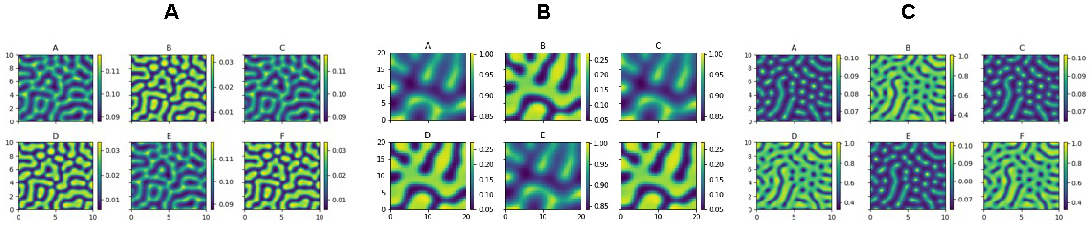
\includegraphics[width=1\textwidth]{chapters/Chapter 2/square_turing}
    \caption{\textbf{Examples of Turing patterns in the six-node circuit.} Three simulations of the six-equation model with Turing I parameter sets.
    In each solution (A, B, C) there are six images which represent every dependent variable of the model.
    The solver used is the \acrfull{ADI} method with non-growing square domains and reflecting boundary conditions.
    Periodic patterns are observed.}
    \label{fig:square_turing}
\end{figure}

\subsection{Increasing Turing robustness by matching consequent dose-response curves}\label{balancing}
One of the aims of the model is
to understand
how to increase the robustness for Turing pattern formation \textit{in-silico} before the experimental work.
This way, we can then use the insights to maximise the chances of finding Turing patterns \textit{in-vitro}.
In this thesis,
we describe Turing robustness as the volume of the parameter space leading to Turing I and Turing I Hopf patterns.
Turing I Hopf patterns are included in this definition as in the context of the six-equation model and the parameters used, they seem to always produce periodic stationary patterns.
This can be seen in the following chapter where we explore these solutions numerically (see Fig.~\ref{system_class_simulations}).

The first approach consisted in investigating how a well-balanced circuit improves the likelihood of patterning.
Once the components of the circuit are put together inside the cell,
these components might not necessarily match well together.
Gene circuits, as opposed to digital circuits, do not have binary inputs and outputs.
Instead, gene expression is regulated continuously,
where a continuous increase in inducer leads to a continuous change in protein concentration
as seen in the dose-response curves of Fig.~\ref{fig:balancing}A
(left).
In this case, inducer [A0*] determines how much [A1*] is produced with a sigmoidal relationship.
The dose-response function is modelled with Hill terms as seen in Eq.\ref{eq:theta}.
A well-matched transfer function occurs when the protein expression levels stemming from dose-response 1
(Fig.~\ref{fig:balancing}A (left))
are compatible with the sensitivity of the regulatory components they act on for dose-response 2
(Fig.~\ref{fig:balancing}A (right)).
For example, a transfer function is not ‘matched’
when a very sensitive promoter is completely turned on even with background levels of activator.
This can occur experimentally
if the background levels of the activator are sufficiently high because of a leaky promoter or strong RBS.
In this case, an induction of the activator above the background would not result in further activation,
leading to a loss of dynamic range (Fig.~\ref{fig:balancing}C (red)).


\begin{figure}[H]
    \centering
    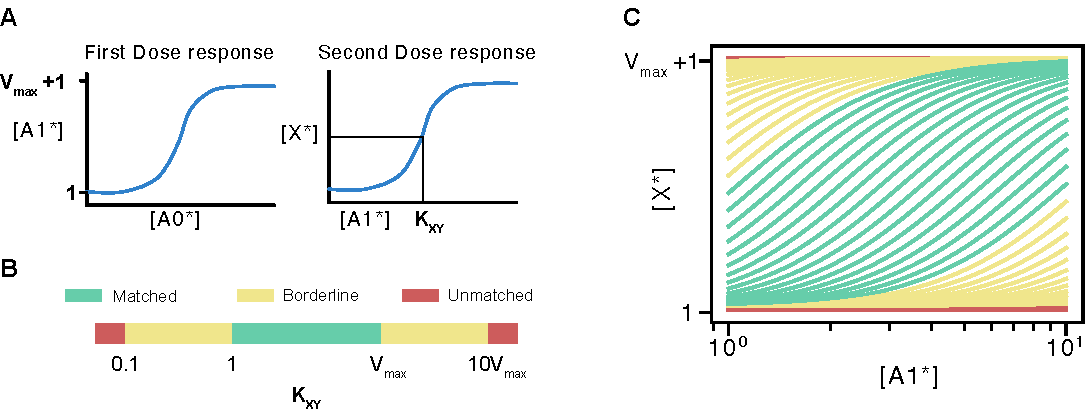
\includegraphics[width=1\textwidth]{chapters/Chapter 2/balancing}
    \caption{\textbf{Balancing of dose-response curves for an inducer-dependent activation.} \textbf{(A)} The first dose-response curve (left) describes the [A0*] dependent production of [A1*] which can vary from $1$ to $V_{\max}+1 $. [A1*], which is the output of the first dose-response, serves as an input for the second dose-response (right). The second dose-response curve describes the [A1*] dependent production of [X*]. The transfer function of the two dose-response curves is said to be balanced or matched if $K_{XY}$ is within the bounds [A1*]. \textbf{(B)} Diagram showing the values of parameter $K_{XY}$ from the second dose-response which generates unmatched (red), borderline matched (yellow), and matched (green) transfer functions. These parameters are with respect to $V_{\max}$ from the first dose-response. \textbf{(C)} Dose-response curves are generated with parameters from the three regions in (B). Matched dose-response curves (green) are the most sensitive to inducer, showing the biggest dynamic range.}
    \label{fig:balancing}
\end{figure}


Mathematically, to ensure a transfer function is matched,
the $K^*_{XY}$ of the second dose-response producing X needs
to be within the dynamic range of the dose-response 1 producing A1 as seen in Fig.~\ref{fig:balancing}A.
The lower bound is the steady state $[X^*]_{ss0}$ when the gene is completely turned off, $\theta=0$.
The upper bound is the steady state $[X^*]_{ss1}$ when the gene is completely turned on, $\theta=1$.
The two bounds can be obtained
by replacing $\theta$ by 0 or 1 and finding the steady state where the derivative is zero so
\begin{equation}
    [X^*]_{ss0}=1; \quad [X^*]_{ss1}=1+V^*_{max}
    \label{1toVmax}
\end{equation}


In the dimensionless model,
both $[X^*]$ an $K^*_{XY}$ are unitless (Table~\ref{tab:Dimensionless_params}) and can be compared. Additionally, the steady state is only dependent on $V$ as opposed to the original model where is dependent on $b$, $V$ and $\mu$.
The transfer function of A1 to X is said
to be matched with a downstream component if $K^*_{XY}$ is between the upper and lower bounds as

\begin{equation}
    1 \leq K^*_{XY} \leq (1+V^*_{X})
\end{equation}

In Fig.~\ref{fig:balancing}B, the green region corresponds to those parameter ranges.
Additionally, in Fig.~\ref{fig:balancing}C,
the green curves correspond to dose-response curves where the transfer function is matched.
The closer $K^*_{XY}$ is to these upper and lower bounds,
the less balanced the upstream component is with the downstream component.
For example, with $K^*_{XY}$ smaller than 1,
given that $[X^*]$ can never approach a value smaller than its basal level of 1 at steady state, $[X^*]$
would always be high enough to cause near-maximal regulation of the downstream component.
On the other hand, with $K^*_{XY}$ larger than $(1+V^*_{X})$, $[X^*]$
could never become high enough to cause near-maximal regulation of the downstream component.
Other two ranges are defined which are borderline matched and unmatched (Fig.~\ref{fig:balancing}B).
As seen in Fig.~\ref{fig:balancing}C,
borderline curves are almost not affected by the inducer and unmatched curves are not affected at all.

The parameter space defined in the previous chapter is divided into these three categories
(matched, borderline and unmatched).
Linear stability analysis was carried out on the three categories
to understand if matching transfer functions would increase the volume of Turing parameter space.
Just by matching the transfer functions,
the robustness goes up by 20-fold which is a significant increase
(see Fig.~\ref{fig:balancing_robustness}) compared to non-balanced circuits.


\begin{figure}[H]
    \centering
    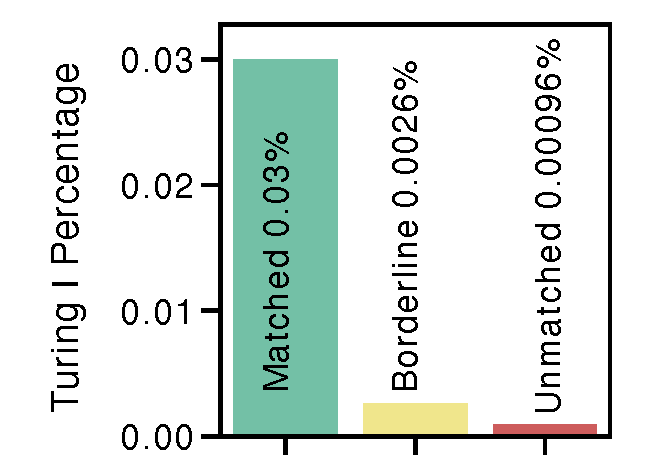
\includegraphics[width=0.6\textwidth]{chapters/Chapter 2/balancing_robustness}
    \caption{\textbf{Turing robustness as a percentage of parameter space with respect to matching of dose-response curves.} Turing instabilities include Turing I and Turing I-Hopf. Robustness from matched to unmatched increases 20-fold.}
    \label{fig:balancing_robustness}
\end{figure}

Following these insights, the transfer functions of the circuit components were matched experimentally by tuning the plasmid copy number,
the strength of ribosome binding sites (RBSs),
start codons and degradation tags~\parencite{Andersen1998, Wang2011,Hecht2017} by Dr.~Jure Tica and Tong Zhu.
Transfer function matching yielded a well-functioning circuit with a better capacity to produce spatial patterns
as discovered in this modelling study.
The matched dose-response curves can be seen in the next section in Fig.~\ref{fig:dose_response_experimental}.


\subsection{Parameter fine-tuning of the gene circuit to increase the likelihood of Turing patterns}
Another way of increasing the Turing parameter space is to tune parameters independently.
In this section, we explore the distribution of obtained Turing parameter sets
to understand how to tune each one to increase the robustness of our system.
Using the literature distribution defined above with only matched
parameter sets, we perform linear stability analysis to find Turing parameter sets.
In Fig.~\ref{fig:param_distributions_turing_vs_noturing},
we can observe how the distribution of Turing samples differs from the general sampling for each dimensionless parameter of the model.

\begin{figure}[H] % h! is a placement specifier; it tries to place the image here.
    \centering
    \begin{adjustbox}{center}
        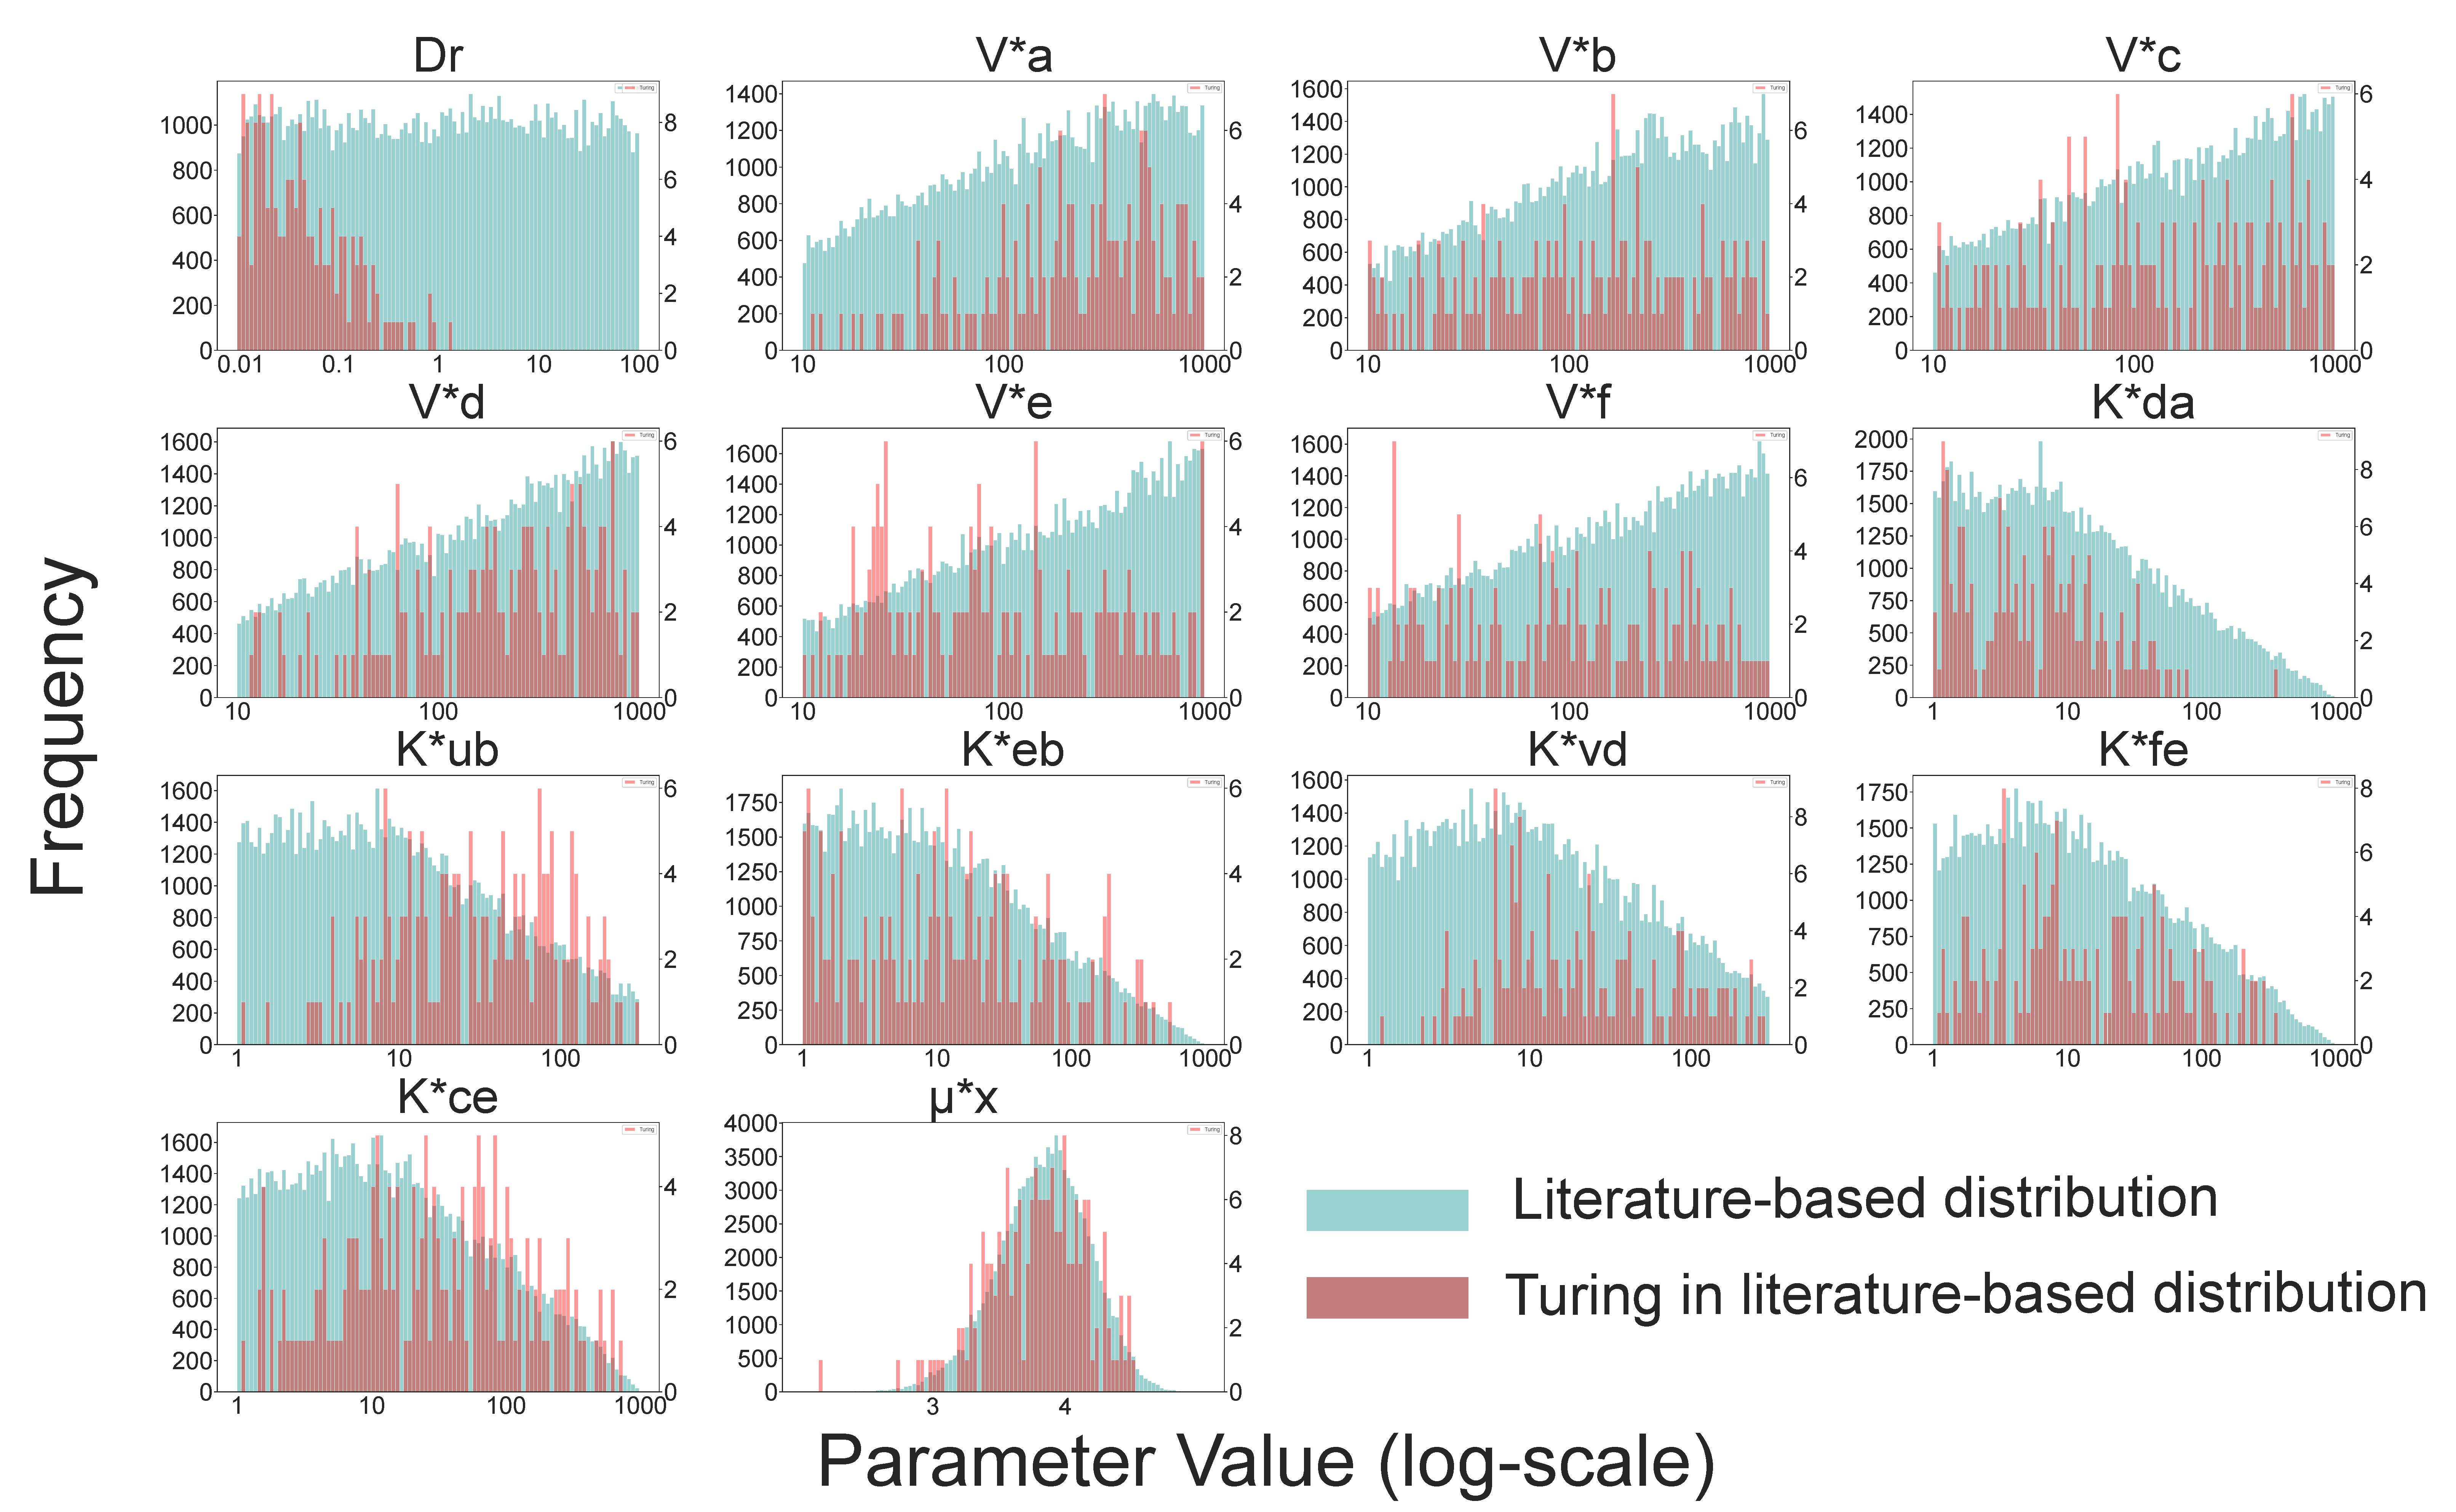
\includegraphics[width=1.2\textwidth]{chapters/Chapter 2/param_distributions} % The name of your image file; assumes it is in the same directory as your .tex file
    \end{adjustbox}
    \caption{\textbf{Broad literature-based distributions for model parameters} Distributions for dimensionless parameters of the model based on literature ranges.
    Blue distributions correspond to the sampled literature-informed distributions,
    where we made sure to only consider parameters where all the circuit transfer functions are matched.
    Red distributions correspond to Turing instabilities found in the blue distributions using linear stability analysis. Turing instabilities include Turing I and Turing I-Hopf. n's are ignored because they are fixed.}
    \label{fig:param_distributions_turing_vs_noturing} % A label for referencing this figure later in the document
\end{figure}

Turing pattern systems appear to have a bias for certain regions of parameters (Fig.~\ref{fig:param_distributions_turing_vs_noturing} red).
This is very clear for diffusion, where Turing patterns usually appear in regions with $D_r$ < 1.
$D_r$ is ($D_V / D_U$) meaning $OC_{14}$ should diffuse slower than pC.
Experimentally, the $D_{OC14}/D_{pC}$ ratio has been measured to show it is 0.25 (unpublished work,~\cite{tica_diffusers}).
This means our experimental setup has a diffusion ratio which is favourable for Turing pattern formation.
%where the DOC14/DpC ratio is approximately 0.25 in agar (1.4% w/V, 37 ºC) (Tica et al., unpublished observations).

Additionally, we used the model to study how to fine-tune the circuit using the exogenous tuning molecules IPTG, aTc and DAPG to increase Turing pattern likelihood.
$K_{da}^*$  and $K_{ce}^*$ are dependent on IPTG and aTC respectively, through an increasing function,
as seen in Eq.~\ref{kda_iptg} and Eq.~\ref{kce_atc}.
Therefore,
to understand the effects of these two exogenous tuning molecules we can look at their respective K parameters.
$K_{da}^*$ Turing parameters have a similar distribution to the sampled distribution,
implying that IPTG does not affect the robustness of the gene circuit to Turing pattern formation.
On the other hand, the $K_{ce}^*$ Turing parameters are more skewed to higher values than in the sampled distribution,
suggesting that aTc increases robustness for Turing pattern formation.
This is further shown by a more extensive sampling of the same distribution with five different $K_{ce}^*$ values
and measuring the Turing robustness in each
(Fig.~\ref{fig:atc_robustness})

\begin{figure}[H] % h! is a placement specifier; it tries to place the image here.
    \centering
    \begin{adjustbox}{center}
        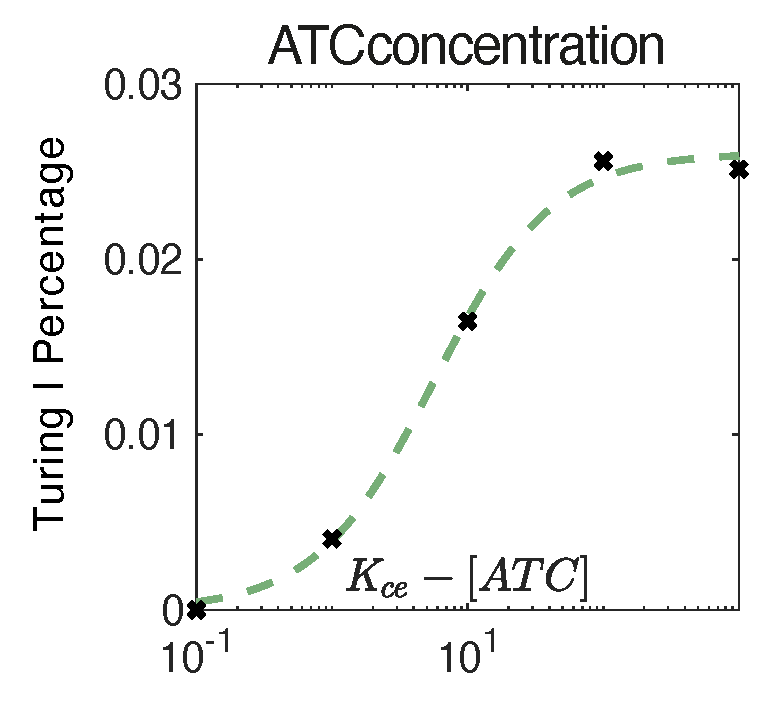
\includegraphics[width=0.5\textwidth]{chapters/Chapter 2/atc_robustness} % The name of your image file; assumes it is in the same directory as your .tex file
    \end{adjustbox}
    \caption{\textbf{Turing I robustness as a function of aTc or $K_{ce}$.} The highest Turing robustness is 0.025 with a high $K_{ce}$ value of $10^2$. After this, robustness plateaus or decays slightly. }
    \label{fig:atc_robustness} % A label for referencing this figure later in the document
\end{figure}

Finally, DAPG increases diffusor degradation by increasing $\mu_u$ and $\mu_v$,
however, these parameters are hidden in the dimensionless model,
where the diffusor equations were integrated into the protein equations.
As seen in Eqs~\ref{six_eq_dimensionless}b,d,f; $\mu_u$
and $\mu_v$ have a positively linear relationship with $K_{ub}^*$ and $K_{vd}^*$, respectively.
Both $K_{ub}^*$ and $K_{vd}^*$ have skewed distributions towards higher values compared to the sampled distribution
(Fig.~\ref{fig:param_distributions_turing_vs_noturing}).
This means that adding exogenous DAPG could also increase the robustness of the circuit for pattern formation.

In this section, we have obtained insights into parameter tuning
to understand how to optimise robustness for Turing pattern formation.
Following guidance from the model,
experimentalists went on to match the transfer functions of the circuit components and add high levels of aTc (10nM aTc).
Before testing the circuit for patterning,
experimentalists tested the behaviour of the circuit in liquid culture to make sure it behaved according to the design,
and that the transfer functions were matching.
Because the full circuit contains many closed-feedback loops, full-circuit liquid culture results are hard to interpret.
Hence,
subcircuit controls with no closed feedback loops were investigated
instead to test whether the circuit was well-matched and behaved as expected.
The conditions tested were under high aTc.
Some relevant subcircuits tested can be seen in Fig.~\ref{fig:dose_response_experimental} left.
The three subcircuits show how the dose-reponse curves are within the responsive ranges, as the green and red curves act according to the other (Fig.~\ref{fig:dose_response_experimental} right).
This means meaning the $K$ and $V$ parameters are within the matched region.
Subcircuit \#2 shows how the circuit is responsive to aTc which means aTc can be used for optimising Turing pattern robustness.

\begin{figure}[H] % h! is a placement specifier; it tries to place the image here.
    \centering
    \begin{adjustbox}{center}
        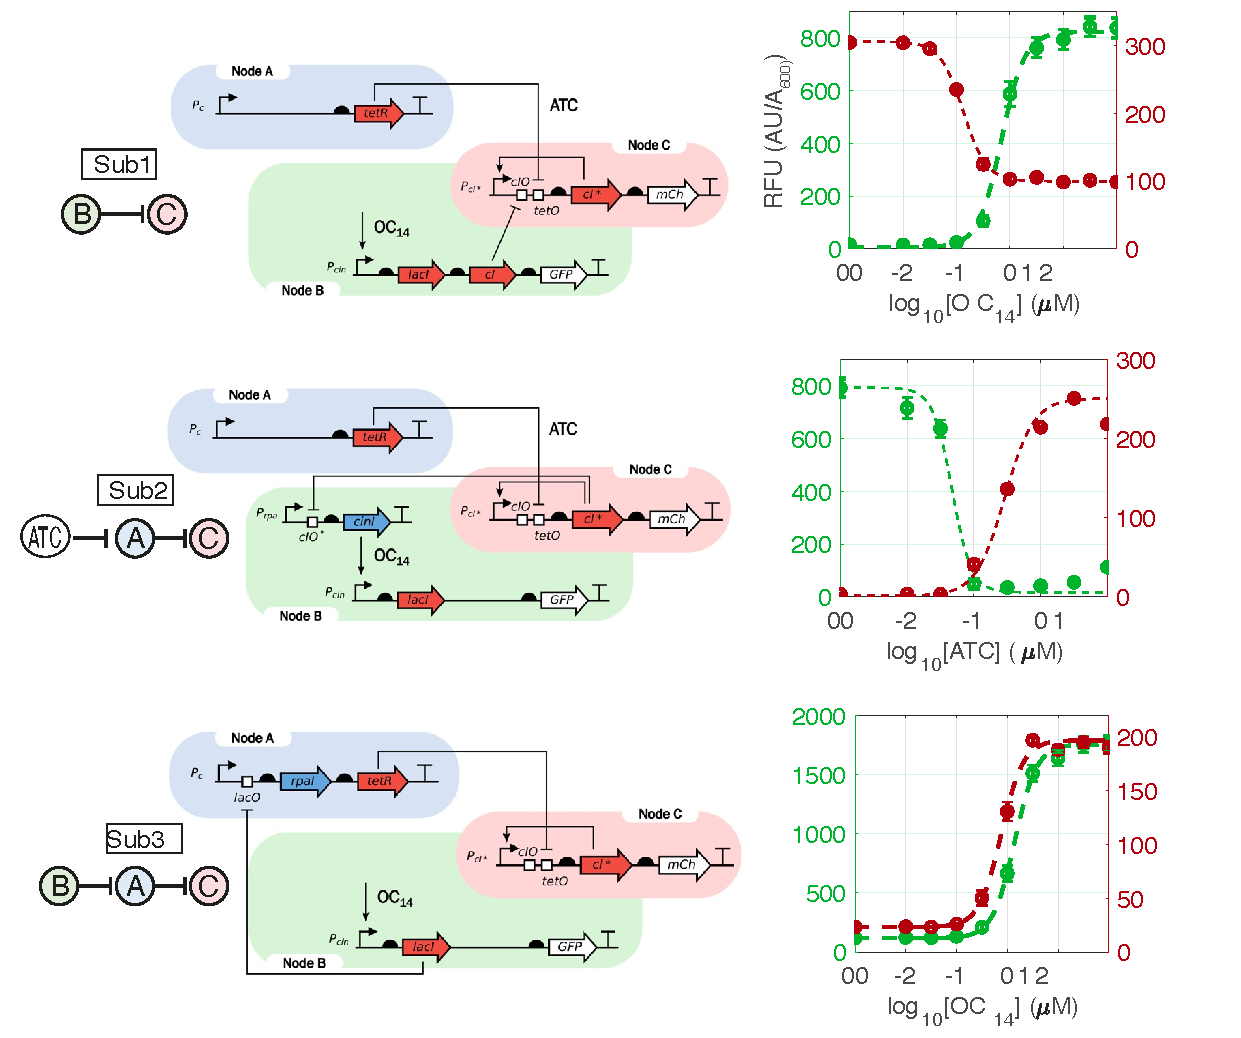
\includegraphics[width=1\textwidth]{chapters/Chapter 2/dose_response_experimental} % The name of your image file; assumes it is in the same directory as your .tex file
    \end{adjustbox}
    \caption{\textbf{Dose-response curves of subcircuits.}
    On the left, the three subcircuits Sub1, Sub2 and Sub3 are shown, which test interactions of the circuit. On the right, the dose-response curves correspond to each subcircuit produced by Dr.~Jure Tica and Dr.~Georg Wachter. Each curve shows liquid culture fluorescence in RFU units (y-axis) 18 hours after induction with different levels of inducer (x-axis).
    GFP on the left and mCherry on the right axis (unit AU/A600, mean ± SEM, n = 3). We can see all dose-response curves are matched as in Sub1 and Sub3, red responds to the green and in Sub2 green responds to the red. Sub1 and Sub3 were tested under 10nM aTc.}
    \label{fig:dose_response_experimental} % A label for referencing this figure later in the document
\end{figure}
\section{Constrained parametrised distributions:
fitting to liquid culture data of gene subcircuits}\label{Constrained parametrised distributions: fitting to liquid culture data of gene subcircuits}
The dose-response curves obtained (Fig.~\ref{fig:dose_response_experimental} left)
are not only useful to characterise the circuit,
but also for the parametrisation of the model.
Using the dimensionless model,
the fluorescence dose-response curves \#1 and \#3 can be fitted
to obtain values for $K_{XY}$ and $V_{X}$ using a multivariate analysis approach.
This is possible because the non-dimensionalisation facilitates the comparison between the model and experimental dose-response curves with simple and intuitive methods.


\subsection{Steady-state subcircuit equations for fitting.}
As previously seen in Eq.\ref{1toVmax},
the non-dimensionalisation transforms the dose-response range so it goes from 1 to $V_{X}+1$.
This transformation can be seen in Fig.~\ref{fig:dose_response_transforms}, right.
For the experimental data to match the model,
it is divided by the smallest fluorescence value within each experiment and is expressed in relative fold-change units
(Fig.~\ref{fig:dose_response_transforms}, left).
Fold-change units can take values from 1 to $F_{\max}/F_{\min}$
(maximal and minimal fluorescence levels in the original, untransformed dataset, respectively).
Because the dose-response curves of subcircuit \#1 and subcircuit \#3 are OC14-dependent, the experimental OC14 units (µM) are also non-dimensionalised using the transform
\begin{equation}
    [B*]=[OC_{14}] \cdot \frac{\mu_{b}\mu_{v}}{k_{2}b_{B}}
    \label{Btransform}
\end{equation}
Now the dimensionless model dose-response curves and experimental dose-response curves are both expressed on relative scales and are compatible for fitting (Fig.~\ref{fig:dose_response_transforms}, bottom).
\begin{figure}[H] % h! is a placement specifier; it tries to place the image here.
    \centering
    \begin{adjustbox}{center}
        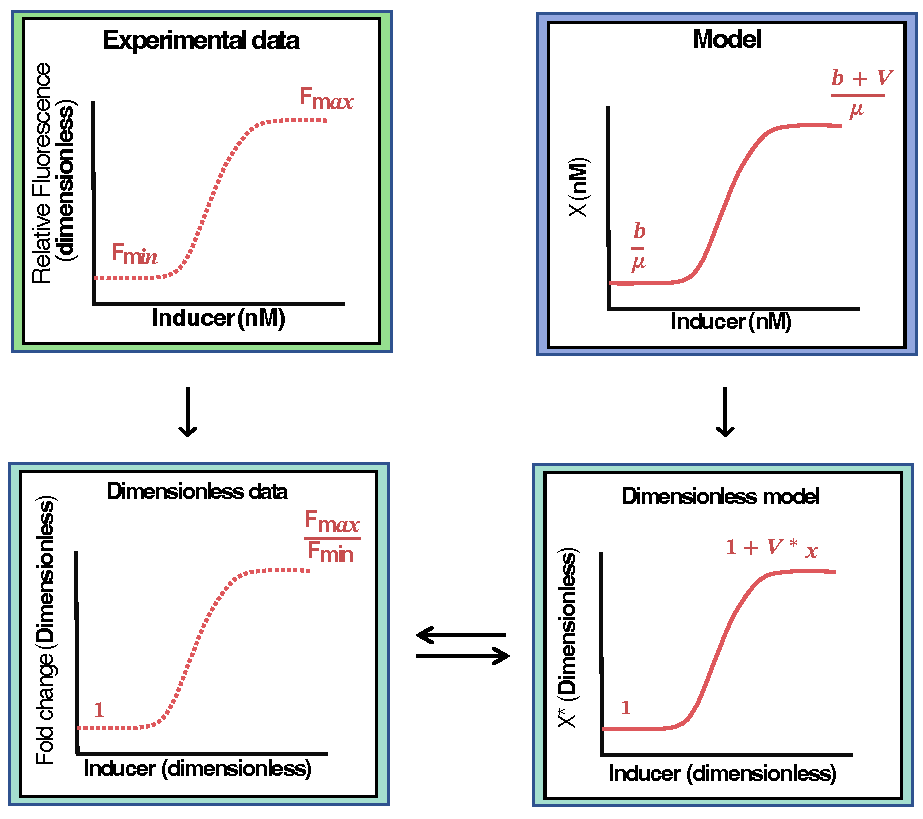
\includegraphics[width=0.8\textwidth]{chapters/Chapter 2/dose_response_transforms}
    \end{adjustbox}
    \caption{\textbf{Experimental data and model transformation for parametrisation.} Experimental data is scaled by the smallest fluorescence value, so the minimum value is 1 (left). The model is nondimensionalised
    as explained in the sections above so the smallest value is 1
    and biggest is $V_{X} +1$ (right).
    In both cases, units are dimensionless, and the basal level is 1 (bottom).}
    \label{fig:dose_response_transforms}
\end{figure}


The models for the subcircuits are derived from the main PDE system (Eqs.~\ref{six_eq_dimensionless}).
Subcircuit \#1 only involves species [F] and [E] (cI and cI*), whereas subcircuit \#3 involves species [C], [D] and [E]
(TetR, LacI and cI*).
Detailed diagrams of these two subcircuits can be found in Fig.~\ref{fig:dose_response_experimental} left.
All other species are set to zero.
For the model parametrisation, based on the subcircuit designs,
we derive steady-state expressions for the dynamically regulated species so that
\begin{equation}
    \pdv{X}{t}=0; \quad X=X_{eq}
\end{equation}

For Subcircuit \#1 we obtain the following steady-state expressions:

\begin{subequations}\label{Subcircuit 1 equations}
\begin{equation}
    F_1 = 1 + V_f \left( \frac{1}{1+ \left( \frac{\mu_v K_{vd}}{k_v [O_{C14}]} \right)^{n_{vd}}} \right)
\end{equation}
%\begin{equation}
%    E_1 = 1 + V_e \left( 1+ \left( \frac{1 + V_f \left( \frac{1}{1+ \left( \frac{\mu_v K_{vd}}{k_v [O_{C14}]} \right)^{n_{vd}}} \right)}{K_{fe}} \right)^{n_{fe}} \right)^{-1}
%\end{equation}
\begin{equation}
    E_1 = 1 + V_e \left( \frac{1}{1+ \left( \frac{F_1}{K_{fe}} \right)^{n_{fe}}} \right)
\end{equation}
\end{subequations}

For Subcircuit \#3 we obtain the following steady-state expressions:
\begin{subequations}\label{Subcircuit 3 equations}
\begin{equation}
    D_3 = 1 + V_d \left( \frac{1}{1+ \left( \frac{\mu_v K_{vd}}{k_v [O_{C14}]} \right)^{n_{vd}}} \right)
\end{equation}
\begin{equation}
    C_3 = 1 + V_c \left( \frac{1}{1+ \left( \frac{D_3}{K_{da}} \right)^{n_{da}}} \right)
\end{equation}
\begin{equation}
    E_3 = 1 + V_e \left( \frac{1}{1+ \left( \frac{C_3}{K_{ce}} \right)^{n_{ce}}} \right)
\end{equation}
\end{subequations}

\subsection{Fitting process and the resulting best-fit distributions.} \label{Fitting process and the resulting best fit distributions.}
In addition to scaling and nondimensionalising, the lowest GFP data points were excluded,
because fluorescence readings were insufficiently sensitive
to measure concentration at these points (Fig.~\ref{fig:dose_response_experimental}).
This improved the quality of the fit and allowed us to identify a broader range of suitable solutions.

The two-equation systems Eqs.~\ref{Subcircuit 1 equations},\ref{Subcircuit 3 equations}
are fitted independently to the experimental dataset with the python \textit{scipy.optimize.curve\_fit} package,
which uses the Levenberg-Marquardt to minimise the sum of squared errors (SSE), given by
\begin{equation}
    SSE = \sum_{i=1}^{i} (y_{i}-f(x_{i}))^2
\end{equation}

where $y_i$ is the experimental data
and $f(x_i)$ are the two systems of equations
parameterised by $V^*_{C}$, $V^*_{D}$, $V^*_{E1}$, $V^*_{E3}$, $V^*_{F}$, $K^*_{vd}$, $V^*_{fe}$, $V^*_{da}$
and $V^*_{ce}$.
The minimisation algorithm generates a vector of best-fit parameters $k$

\begin{table}[H]
    \centering
    \begin{tabular}{|c|c|c|c|c|c|c|c|c|}
        \hline
        \textbf{$V^*_{C}$} & \textbf{$V^*_{D}$} & \textbf{$V^*_{E1}$} & \textbf{$V^*_{E3}$} & \textbf{$V^*_{F}$} & \textbf{$K^*_{vd}$} & \textbf{$V^*_{fe}$} & \textbf{$V^*_{da}$} & \textbf{$V^*_{ce}$} \\
        \hline
        9.95 & 6.50 & 1.99 & 7.8 & 3.64 & 18.94 & 2.26 & 67.92 & 3.47 \\
        \hline
    \end{tabular}
    \caption{\textbf{Vector of best fit parameters $k$}}
    \label{table:bestfit table}
\end{table}


Two best-fit parameters are obtained for $V^*_{E}$ as this parameter is present in both subcircuit models.
However, only $V^*_{E1}$ from subcircuit \#1 is considered.
These parameters are used to generate the following dose-response curves (Fig.~\ref{fig:dose_responses_bestfit}).


\begin{figure}[H] % h! is a placement specifier; it tries to place the image here.
    \centering
    \begin{adjustbox}{center}
        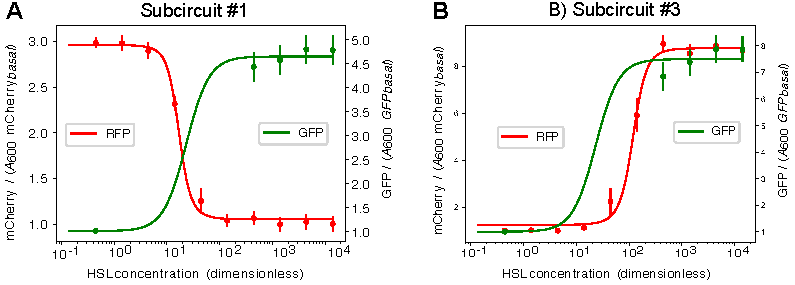
\includegraphics[width=1\textwidth]{chapters/Chapter 2/dose_responses_bestfit} % The name of your image file; assumes it is in the same directory as your .tex file
    \end{adjustbox}
    \caption{\textbf{Best fit for processed data set.} Processed dataset is fitted using \textbf{(A)} Eq.~\ref{Subcircuit 1 equations} for subcircuit \#1 and \textbf{(B)} Eq.~\ref{Subcircuit 3 equations} for subcircuit \#3.}

    \label{fig:dose_responses_bestfit} % A label for referencing this figure later in the document
\end{figure}


The minimisation algorithm produces a covariance matrix $C_k$. This covariance matrix can also be understoood as the inverse of the Hessian matrix which represents the derivative of the loss function in the different parameter dimensions.
In other words, this Hessian matrix represents how the loss increases or decreases when parameters are varied together

\begin{equation}
    H_{L_{k}} = \begin{bmatrix}
                     \frac{\partial^2 L}{\partial k_1^2} & \frac{\partial^2 L}{\partial k_1 k_2} & \cdots & \frac{\partial^2 L}{\partial k_1 k_{n}} \\
                     \frac{\partial^2 L}{\partial k_2 k_1} & \frac{\partial^2 L}{\partial k_2^2} & \cdots & \frac{\partial^2 L}{\partial k_2  k_{n}} \\
                     \vdots & \vdots & \ddots & \vdots \\
                     \frac{\partial^2 L}{\partial k_{n}k_1} & \frac{\partial^2 L}{\partial k_{n}  k_2} & \cdots & \frac{\partial^2 L}{\partial k_{n}^2}
    \end{bmatrix}
\end{equation}


A multivariate Gaussian distribution is generated using $k$ and $C_{k}$
\begin{equation}
    X \approx N(k,C_k)
\end{equation}

with a probability density function $p(x;k,C_k )$

\begin{equation}
    p(x;k,C_k )= \frac{\exp\left(-\frac{1}{2} (x - k)^\top C_k^{-1} (x - k)\right)}{\sqrt{(2\pi)^k C_k}}
\end{equation}

The multivariate Gaussian distribution is the generalization of a normal distribution to higher dimensions.
For example, for 2-dimensional Gaussian distributions,
when the covariance of two parameters X and Y is positive, the parameters are positively correlated
(Fig.~\ref{fig:multivariate_gaussians}, right).
This means that if the parameters are increased together, the behaviour of the system should change minimally
(and the error to the data should not increase).
On the other hand, a negative covariance leads to an inverse correlation of the parameters,
meaning when one increases the other should decrease to ensure the error does not increase
(Fig.~\ref{fig:multivariate_gaussians}, left).
Finally, a covariance of zero means the X and Y parameters are completely independent,
producing a circular distribution (Fig.~\ref{fig:multivariate_gaussians}, center).

\begin{figure}[H] % h! is a placement specifier; it tries to place the image here.
    \centering
    \begin{adjustbox}{center}
        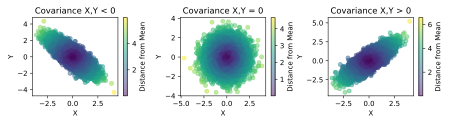
\includegraphics[width=1\textwidth]{chapters/Chapter 2/multivariate_gaussians} % The name of your image file; assumes it is in the same directory as your .tex file
    \end{adjustbox}
    \caption{\textbf{Multivariate Gaussian distributions.} Pairplots of X and Y parameter distributions with (left) negative covariance, (centre) zero covariance and (right) positive covariance.
    The colour represents the distance to the mean, or in other words to the best-fit parameter ($k$).
    Blue are the parameter ($k$) with minimal loss and yellow are neighbouring parameters with bigger loss.}
    \label{fig:multivariate_gaussians} % A label for referencing this figure later in the document
\end{figure}

The multivariate Gaussian distribution generated from the vector of best-fit parameters $k$ and the covariance matrix $C_{k}$ can be seen as a pairplot in Fig.~\ref{fig:multivariate_from_fit}.
Positive, negative and no correlations were observed in these distributions.
This figure shows how certain parameters have positive covariance such as $V^*_c$ and $K^*_{ce}$.
A high $V^*_c$ indicates a strong production of TetR, while a high $K^*_{ce}$ indicates a higher concentration of TetR to have the same inhibition effects.
Therefore, if both are increased together, the behaviour of the system should remain the same and the dose-response fit should be unaltered.
Some parameters have a negative covariance such as $K^*_{vd}$ and $K^*_{fe}$.
While a high $K^*_{vd}$ decreases the production of cI, a low $K^*_{fe}$ decreases the amount of cI needed to have the same inhibition effects.
Therefore if varied in opposite directions, the circuit behaviour remains unaltered.
Others are independent like $V^*_{d}$ and $K^*_{f}$ which determine the production rates of the molecules LacI and cI which affect the circuit independently.

\begin{figure}[H] % h! is a placement specifier; it tries to place the image here.
    \centering
    \begin{adjustbox}{center}
        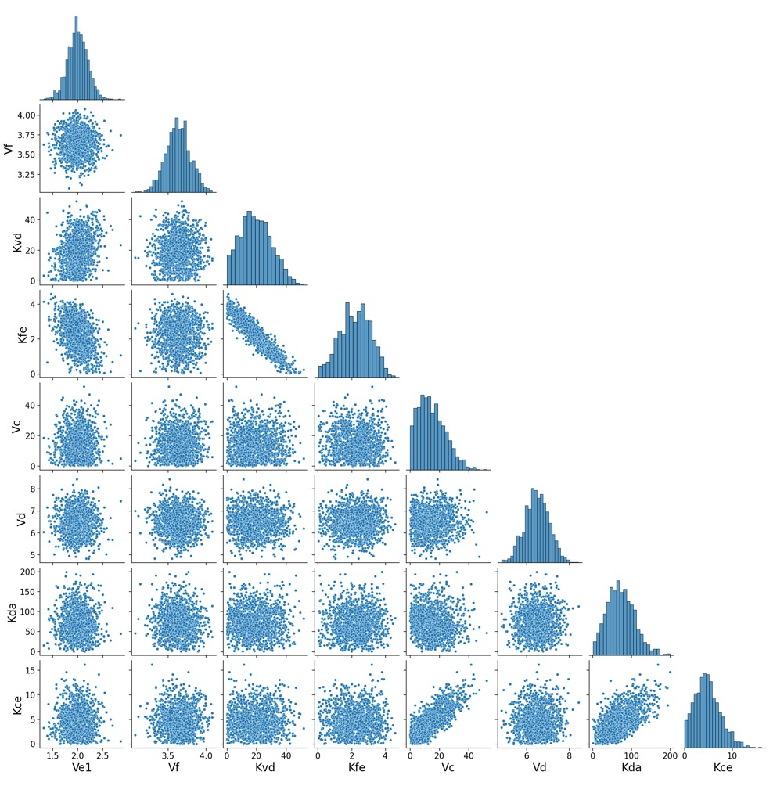
\includegraphics[width=1\textwidth]{chapters/Chapter 2/multivariate_from_fit} % The name of your image file; assumes it is in the same directory as your .tex file
    \end{adjustbox}
    \caption{\textbf{Multivariate Gaussian distributions for fitted parameters.}
    Pairplot of distribution resulting from fitting subcircuit \#1 and \#3, using $q=10$.
    This distribution has a probability density function $p(x;k,10\cdot C_{k})$
        where $k$ is the best fit parameter vector and $C_{k}$ is the covariance matrix.
    Diagonals represent the univariate distributions.
    The non-diagonals represent the multivariate distributions of parameter pairs, where we can observe positive and negative correlations as well as independent pairs of parameters. Negative parameters are removed from the distribution as these are biologically not possible.}
    \label{fig:multivariate_from_fit} % A label for referencing this figure later in the document
\end{figure}

The width of the multivariate Gaussian distributions can be increased by multiplying $C_k$ by a scalar factor $q$ where $q>1$.
This process unconstrains the fits and allows more error with respect to the experimental data.
To search for Turing patterns close to the fitted parameter combination $k$,
the value of $q$ is progressively increased until a Turing parameter set is found through linear stability analysis.
Through this process, the first 3 Turing parameter combinations are found with $q=10$.
These are the closest Turing solutions to the best fit parameter combinations.
The dose-response curves
generated by the $q=10$ distribution are shown in Fig.~\ref{fig:dose_response_multivariate_gaussian}.
Within all the curves shown, 3 of them are generated by Turing parameter sets.
The three Turing parameter sets are ensured to be ‘balanced’,
where the input/output relationships of the components are matched (see Section~\ref{balancing}).

\begin{figure}[H] % h! is a placement specifier; it tries to place the image here.
    \centering
        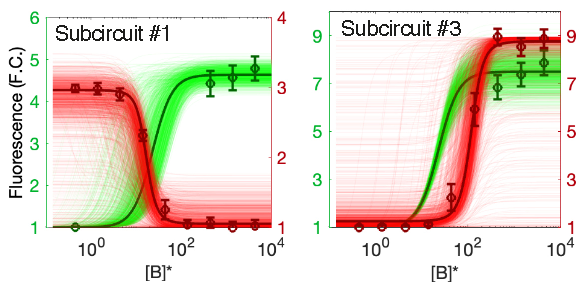
\includegraphics[width=1\textwidth]{chapters/Chapter 2/dose_response_multivariate_gaussian} % The name of your image file; assumes it is in the same directory as your .tex file
    \caption{\textbf{Fitted OC14 dose-response curves
    produced using the multivariate Gaussian distributions.}
    Dots show experimental data,
        the thick line is generated from best fit parameters and the thin lines are derived from multivariate Gaussian distributions cantered around the best fit with $q=10$.
        The parameters used to generate these curves come from the multivariate analysis optimisation, for subcircuit 1 (left) and subcircuit 3 (right). The parameter distributions are shown in Fig.~\ref{fig:multivariate_from_fit}}
    \label{fig:dose_response_multivariate_gaussian} % A label for referencing this figure later in the document
\end{figure}
The corresponding $q=10$ multivariate Gaussian parameter distributions are shown in Fig.~\ref{fig:multivariate_from_fit}.
The distributions of the multivariate Gaussian in 1-parameter dimension and the Turing parameter sets are shown in Fig.~\ref{fig:1d_distributions}.
This figure shows where the parameters of Turing solutions lie in comparison with the fitted distributions.
Overall, only parameter $K^*_{da}$ is far off from the Turing solutions.
Lower values of $K^*_{da}$ would be required to increase the likelihood of finding Turing solutions.
This K*da parameter, which is captured in Subcircuit \#3 (see Eq.~\ref{Subcircuit 3 equations}b), has the highest uncertainty because nodeA is hideden and we therefore need to infer two functions with one curve.
%TODO add starts to params

\begin{figure}[H] % h! is a placement specifier; it tries to place the image here.
    \centering
    \begin{adjustbox}{center}
        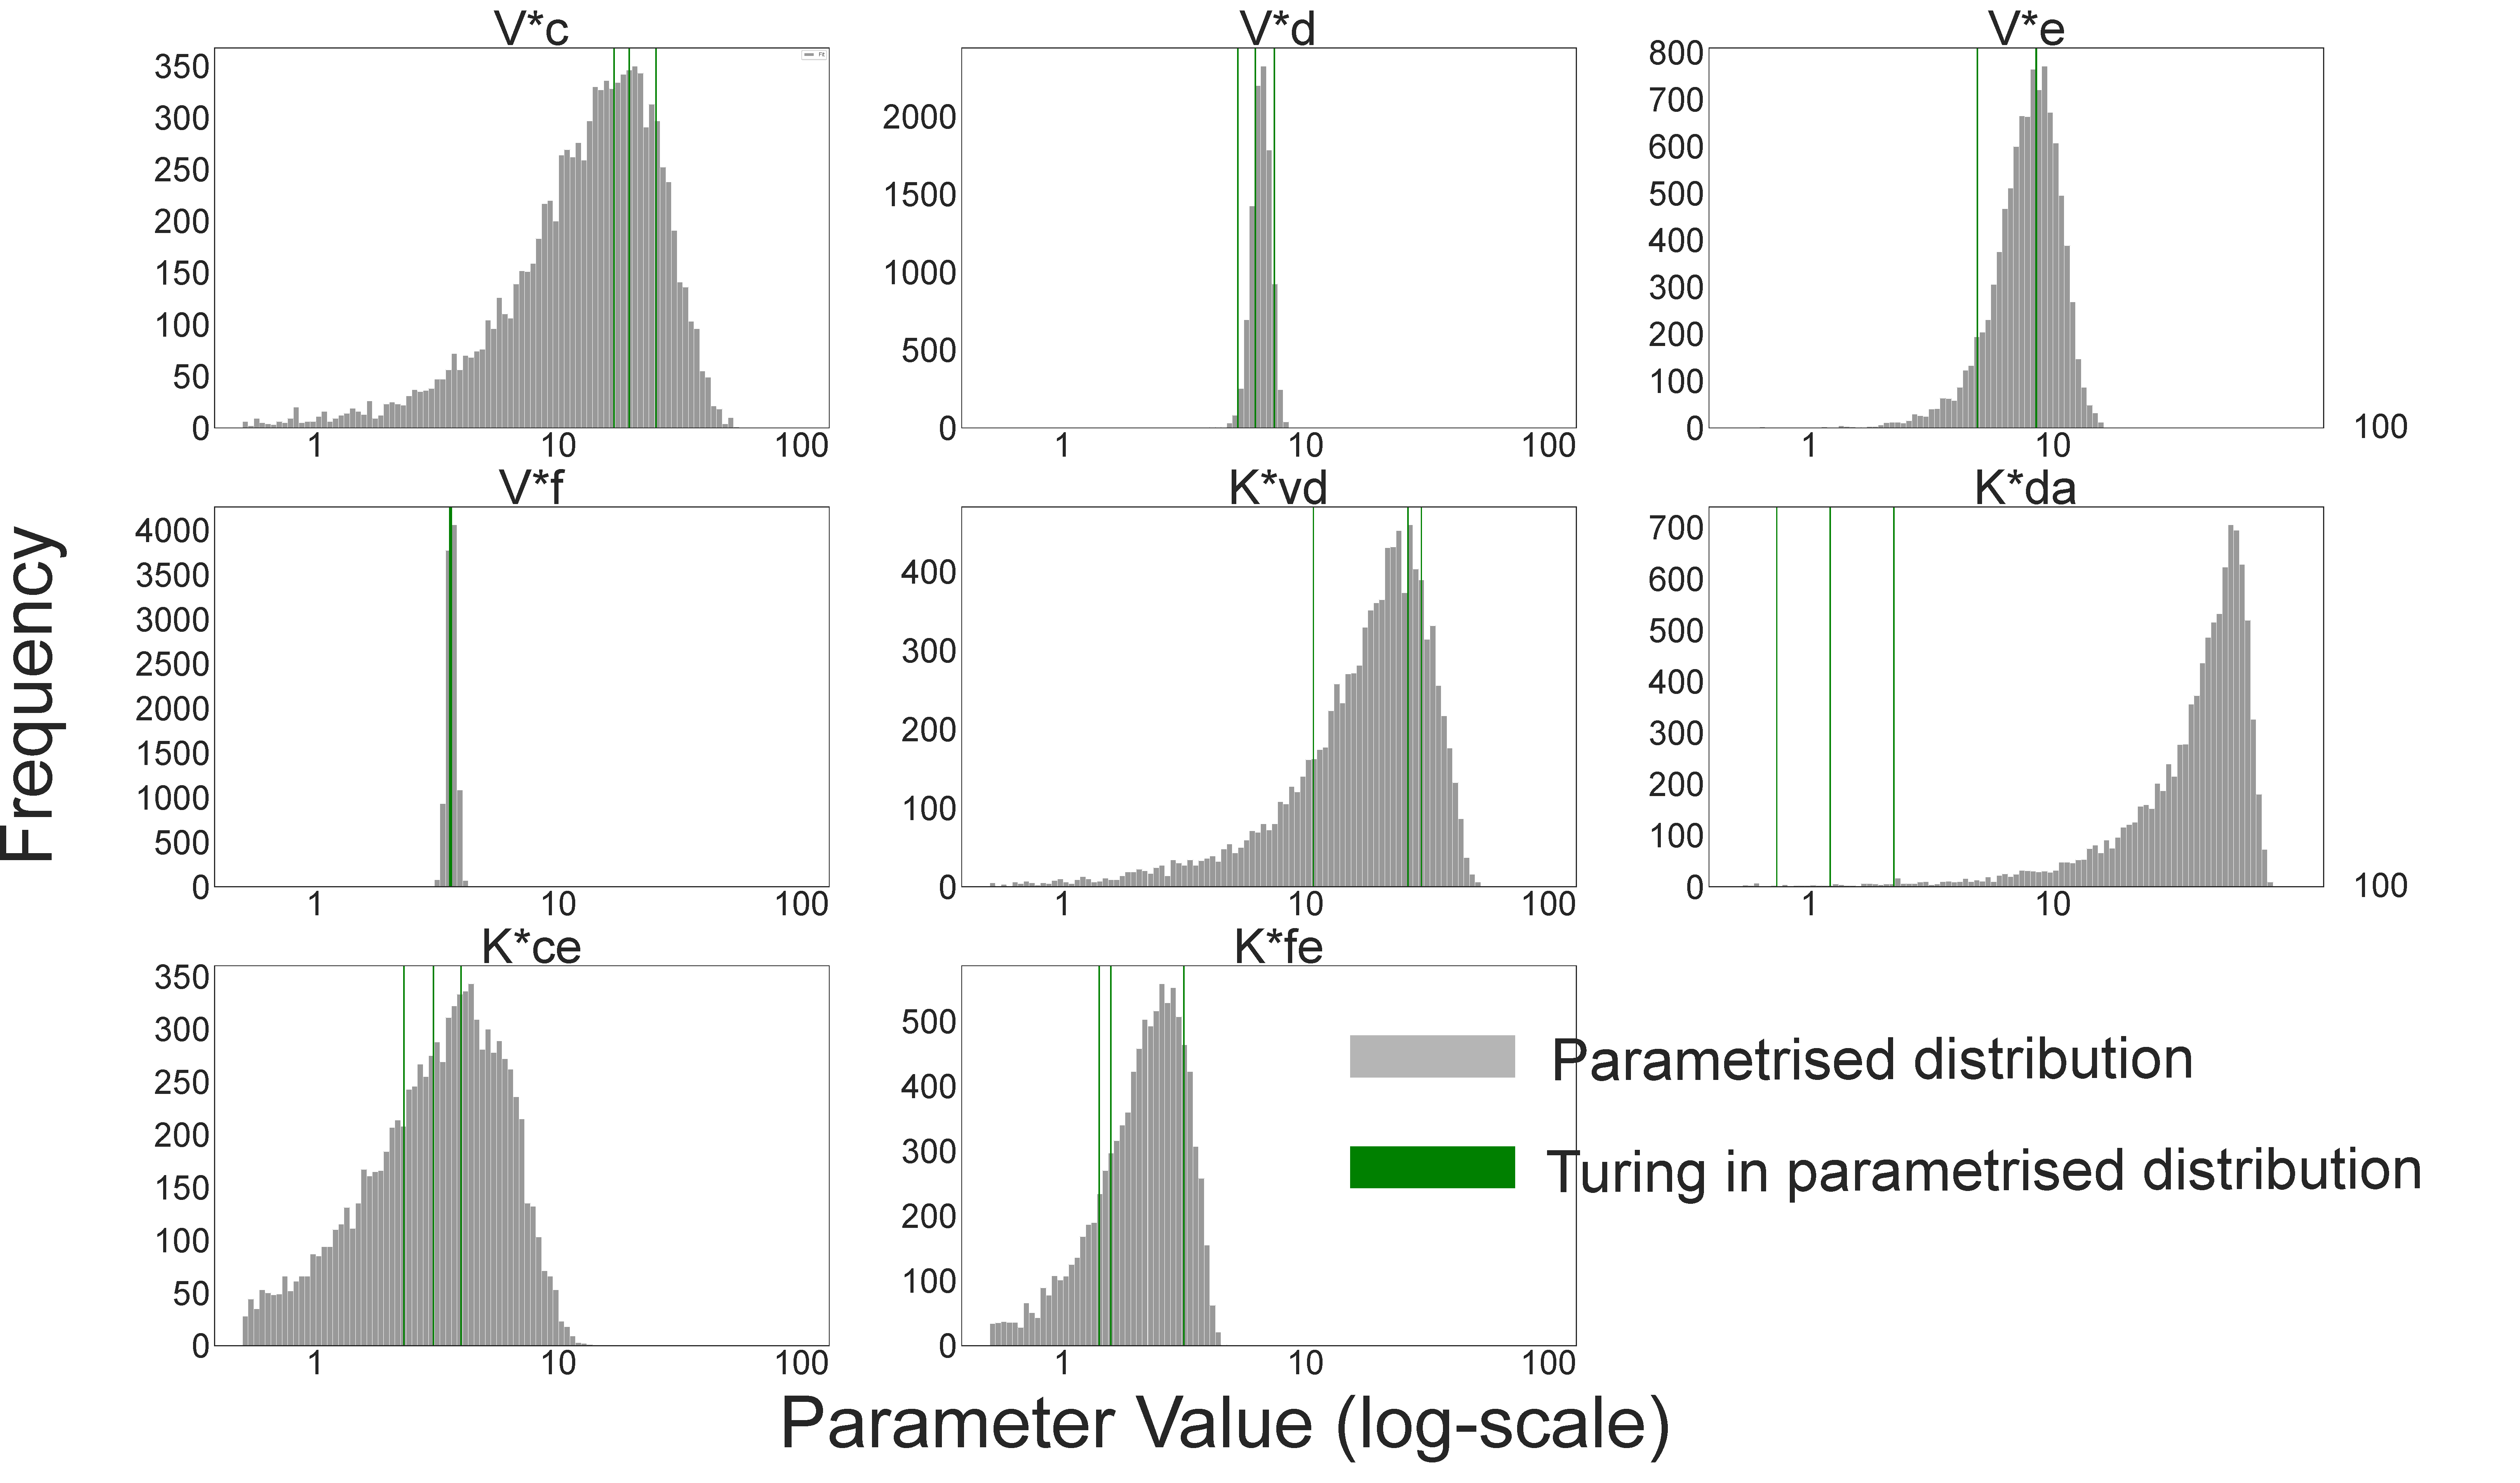
\includegraphics[width=1\textwidth]{chapters/Chapter 2/1d_distributions} % The name of your image file; assumes it is in the same directory as your .tex file
    \end{adjustbox}
    \caption{\textbf{Constrained parametrised distributions for $V^*_X$ and $K^*_{XY}$ parameters in 1 dimension.}
    Distributions for dimensionless parameters based on fitting to liquid-culture experimental data.
    Grey distribution corresponds to parameters from fitting with $q=10$.
    Green vertical lines correspond to the 3 Turing parameter sets
    found in the grey distribution using linear stability analysis. Parameters which generate non-matched dose-response curves are removed.}
    \label{fig:1d_distributions} % A label for referencing this figure later in the document
\end{figure}

\section{Discussion}
A synthetic gene circuit was built with the aim of engineering periodic pattern formation in synthetic \textit{E.~coli} biofilms (Fig.~\ref{fig:synthetic circuit_chapter2}).
This chapter described the model built to understand the spatio-temporal dynamics of this synthetic gene circuit.
The parameter space was explored to show the circuit can produce Turing patterns, and in certain regions, the likelihood of finding these patterns is higher.
Finally, the model was parametrised using liquid culture data to constrain the model parameters to experimentally realistic values.

\subsection{Model of synthetic gene circuit \#1754}
The model presented was a PDE system which describes the concentrations of the six proteins in space and time.
This model gives us insights into how protein concentrations change over time and in space and whether any spatio-temporal patterns form.
Because the experimental circuit is the largest \acrfull{RD} gene circuit ever built, the model is highly complex with many variables and parameters.
This results in computationally expensive numerical simulations and a high-dimensional parameter space with over 20 dimensions, which is complicated to sample.

To simplify the model, many assumptions were made.
For example, quasi-steady states were assumed for mRNA production, protein-promoter binding, receptor-diffusor binding and diffusor synthesis.
Although these processes exist in a quasi-steady state equilibrium, they might produce delays which are not taken into account in this model.
Investigating these delays would be necessary in the future to understand whether they disrupt pattern formation as shown in~\cite{Maini2012}.
Additionally, degradation was assumed to be linear, which might not be accurate in some cases.
High levels of proteins, burden or age-dependent effects might collapse the degradation machinery~\parencite{kintaka2020genetic} leading to non-linear dynamics which are not currently captured.
Additionally, diffusor precursors as well as diffusor receptors were assumed to be in excess to avoid extra equations and parameters.
The parameters of the model were also assumed to be constant over time, which might not be realistic due to cell burden, nutrient depletion or other effects in the biofilm.
Future work in this direction would involve exploring experimentally the relationship between these effects and the model parameters.
An interesting example of this would be to define a time-dependent nutrient equation on which kinetic parameters are dependent.
Finally, this model assumed fluorescent protein concentration is linearly correlated with fluorescence.
Although this assumption is often correct~\parencite{soboleski2005green, csibra2022absolute}, several factors can disrupt the linearity.
For example, low concentrations of fluorescent protein might not be detected by the instruments, leading to a non-linear relationship.
pH and temperature can also affect fluorescent values~\parencite{ward1982spectral}.
When using LacI and cI* to model GFP and RFP fluorescence respectively, we need to take into account these assumptions on linearity and understand when they might break.

\subsection{Finding Turing instabilities and optimising Turing robustness}
Regardless of all the assumptions, the model was extremely useful in giving us insights into the system.
Firstly, the model parameter space was searched using linear stability analysis to find Turing I instabilities.
Turing I-Hopf instabilities were also searched for, as they have been shown to produce stationary periodic patterns in many cases as seen in Section~\ref{nogrowth}.
The model did produce Turing I and Turing I-Hopf instabilities, meaning periodic stationary patterns as the ones observed in Fig.~\ref{fig:square_turing} could occur experimentally.
When the gene circuit was built inspired by the original \#1754 topology,
more nodes and connections had to be implemented to replicate the original functions.
Therefore, it was unclear whether these changes would remove the capabilities of patterning.
Proving the genetic implementation of this topology could produce patterning was necessary before searching for Turing patterns experimentally.

The model also helped understand parameter regimes in which the gene circuit was more likely to produce Turing instabilities, including both Turing and Turing I-Hopf.
By matching circuit components to have responsive dose-response curves, the robustness could be increased 20-fold from 0.001\% to 0.19\% as seen in Fig.~\ref{fig:balancing_robustness}.
This robustness could be further increased by tuning specific parameters such as decreasing the $D_{OC14}/D_{pC}$ ratio, increasing aTc or increasing DAPG.
Different levels of aTc were explored in a system with matched dose-response curves.
It was seen that robustness could be increased from 0 to 0.025 by increasing $K_{ce}$, which is equivalent to adding exogenous aTc to the experiment.

These results guided the experimental fine-tuning of the circuit by matching dose-response curves and adding exogenous aTc and DAPG.
Decreasing $D_{r}$ is harder, as there is no current good method for controlling the diffusion of quorum sensing molecules.
A potential route of decreasing the diffusion rate of a quorum-sensing molecule is through receptor sequestering:
When the number of receptors is much larger than the number of quorum sensing ligands,
there is an irreversible uptake of some molecules which has been linked to shorter range communication (i.e. slower diffusion constants~\parencite{vangestel}).
Therefore, to decrease $D{r}$,
we can slow down the diffusion of $OC_{14}$ by increasing the expression of the CinR receptor which will bind to $OC_{14}$.
This can be done by tuning the RBS for higher expression.

Overall, this model enabled us to design experimental strategies for tuning the robustness of the system so Turing patterns could be obtained experimentally.
However, it is important to note that although they have been optimised, the robustness levels obtained are still extremely low.
Further investigation to understand how to further increase the percentage of Turing solutions in parameter space is needed.
In this thesis, robustness optimisation was carried out by tuning model parameters.
However, it is worth investigating whether growth, boundary conditions or even a pre-pattern could increase the probability of obtaining Turing patterns with this circuit.

\subsection{Model parametrisation}
Working with large parameter spaces based on literature parameters is useful for understanding the overall potential of the circuit architecture.
However, once the system is fine-tuned by matching dose-response curves and adding exogenous aTc, it is important to constrain the parameter space to that of the fine-tuned circuit, so more accurate results are produced.
Additionally, because of the high dimensionality of the parameter space, it is useful to parametrise the model to obtain a smaller parameter space which is easier to sample.
Dose-response curves from the fine-tuned circuit in liquid culture were produced which could be used for parametrisation.
Parametrisation was possible because of the dimensionless model.
This dimensionless model could produce dose-response curves such as the experimental ones by taking the steady state expressions under different inducer concentrations (Eqs~\ref{Subcircuit 1 equations},~\ref{Subcircuit 3 equations}).
Relative fluorescent units from the experimental dose-response curves could be directly compared to dimensionless units of our dimensionless model as seen in Fig.~\ref{fig:dose_response_transforms}.

It is important to note that the experimental data used for parametrisation represents the behaviour of cells in liquid culture.
Parameters might vary slightly for cells growing in colonies on agar surfaces, especially as they become old.
Dose-response curves in agar could be produced in the future.
This would allow us not only to understand the parameters of cells growing in agar dishes, but also have different fits for old cells in the middle and new cells at the edge of the colony.

By fitting the dose-response models to the experimental liquid culture data, we aimed to obtain a distribution of model parameters that replicated the experimental data with a certain level of uncertainty.
A distribution is preferred over a single fit as biological systems exhibit noise and there is a certain level of uncertainty in the fixed parameters of the model.
This distribution could be obtained by using a Bayesian approach or a multivariate Gaussian optimisation approach.
With Approximate Bayesian Computation, a prior is given which is updated by sampling the parameter space to obtain a posterior distribution that fits the data.
This Bayesian approach works well if prior knowledge needs to be incorporated into the model and if non-linear relationships between parameters are present.
However, it is more computationally expensive.
On the other hand, multivariate Gaussian optimisation is a much more computationally efficient algorithm based on a simple least squares minimisation to produce a mean value and a covariance matrix.
This algorithm is less flexible in terms of the prior given and the relationships between parameters (i.e.~non-linearities are not captured).
Additionally, the distribution is only centred around the best fit mean value, meaning the posterior might be limited.

Using the multivariate Gaussian approach, a distribution of parameters was obtained
which fitted the experimental dose-response with a certain level of uncertainty.
This allowed for a much more constrained parameter space which is easier to sample and gives more accurate results.
Additionally, the fitting process allowed us to understand and verify correlations between parameters.
All these correlations can be explained using the logic of the circuit architecture, which means the distributions are correct and the model accurately describes the dynamical behaviour of the circuit.
Interestingly, Turing solutions were found within these distributions.
Theoretically, these Turing solutions are the closest solutions in parameter space that fit the experimental data.
Therefore, we should expect their dynamic behaviour to match the experiments more closely than any other Turing solution found in the literature-based parameter space.

However, a high level of uncertainty ($q=10$) was needed to find such Turing solutions in the distribution.
This lack of robustness in the fitted distribution can be attributed mainly to the $K^*_{da}$ parameter, which has a higher distribution than Turing solutions.
This $K^*_{da}$, which is the $[LacI]$ needed for half repression of node A, is an uncertain parameter as no fluorescent reporters are linked to node A.
Currently, the only data used is on node B, with a GFP reporter, and node
C, with an mCherry reporter.
Having dose-response curves which report on every gene of the circuit would get rid of issues on node A parametrisation, and potentially increase the Turing robustness in the fitted distribution.
A potential route to improve this parametrisation technique would be to use RT-qPCR, which is a technique used for mRNA quantification.
mRNA counts of every one of the six genes would be measured for different inducer concentrations, hence obtaining information on the currently 'hidden' nodes.
Additionally, because fluorescence levels are sometimes not an accurate predictor of protein levels as previously discussed, using mRNA counts would improve issues such as the low fluorescent values not being detected.
Overall, this parametrisation method goes beyond studying pattern formation and could be useful to parametrise any genetic circuit model in synthetic biology.


As we reflect on the work presented in this chapter, the significance of optimizing Turing pattern robustness through precise parameter tuning becomes clear.
Additionally, our parametrization approach and the subsequent uncovering of Turing patterns present within experimentally relevant parameter distributions stand as a testament to the power of using mathematical models in synthetic biology.
The insights gleaned from this study illuminate the path forward not only for the engineering of synthetic \textit{E. coli} biofilms, which is done in the next chapter, but also for the broader engineering of genetic circuits in complex biological systems.
As we continue to fine-tune these parameters, our ability to predict and control the dynamical behavior of synthetic gene circuits will advance, leading to more robust and reliable applications in biotechnology.

    \chapter{Patterning in Synthetic Bacterial Colonies} \label{chapter3}
%Chapter one describes how systems might be more robust for patterning than linear stability analysis predicts, and that we should look for other analytical solutions when considering patterning.
%It also studied how growth and boundaries might change the patterning outcome.
%
%In chapter 2 the patterning capabilities of the gene circuit engineered in ~\cite{Tica2020} were studied.
%It was shown that patterns can arise from this circuit.
%Certain parameter regimes are more robust for patterning, such as matching transfer functions, adding aTc,DAPG or slowing $D_{V}$ diffusion.
%Finally, in chapter 2 the circuit was parametrised using the model under liquid culture experiments which have followed the circuit tuning guidance to optimise Turing robustness.
%%
%Following chapter 2 insights, I carried out spatial experiments were carried out with the optimal tuning conditions.
%In this chapter, chapter 1 and chapter 2 knowledge is combined and spatial experiments  based on our previous work.

Using the insights obtained in the previous chapter, a wide range of microscopy experiments were carried out in optimal turing conditions to obtain patterning in E.coli biofilms.
The aim is to observe fluorescent periodic patterns when these biofilms are observed under the microscope.
The model is key to elucidate which mechanisms are actually behind the patterns, and specifically to investigate if periodic patterns obtained are a result of Turing's mechanism.

In this section, some of the experimental results produced in this thesis are shown.
Further microscopy results done by researchers at the Isalan Lab are also presented.
A framework to simulate numerically reaction-diffusion systems in shaped and growing biofilms is developed to compare model outputs and experimental results.
Finally, perturbation experiments are carried out computationally, to predict experimental perturbations and elucidate the mechanisms of pattern formation.


%
%The aim is to predict pattern formation under the chosen spatial setup which are growing colonies.
%Additionally, for the patterns obtain, the aim is to obtain mechanistic insights of what the patterns can do.
%This is done first with the general parameter distribution from the literature to explore the overall potential of the circuit in bacterial colonies.
%Then, is done in the parametrised distributions to get more specific insights into the mechanisms in the regions we find ourselves in and to have a more predictable model.

\section{Experimental rings in small colonies with high aTc}\label{Rings in small colonies with high aTc}
In the previous chapter, certain conditions which could affect robustness for Turing pattern formation are found.
As already shown, the circuit components were matched by Dr.~Jure Tica and Tong Zhu (see Fig~\ref{fig:dose_response_experimental}) to improve robustness as seen in Fig.~\ref{fig:balancing_robustness}.
In this section, I investigate the circuit in a biofilm using confocal microscopy under those optimal Turing conditions.
More specifically, I look at how the biofilm fluorescent patterns change with different levels of aTc in small colonies

MK01 \textit{E.coli} cells were transformed using electroporation (Section~\ref{electroporation}) with the full circuit.
This involved the introduction of 4 plasmids with the three nodes and the regulator cassette as seen in Fig.~\ref{fig:synthetic circuit_chapter2} and Table~\ref{tab:plasmid table} into our \textit{E.coli} cells.
For this, the cells were then plated in 6 well MatTek plates and grew as individual colonies which are radially growing biofilms.
These growing colonies are then imaged using confocal microscopy.
Confocal microscopy is a type of fluorescence microscopy used to image thicker objects, where the beam of light focuses on one depth level, meaning you can get a single z plane of fluorescence.
This way we can obtain a 2D fluorescence pattern steaming from a single focal plane of the colony ~\parencite{semwogerere2005confocal}.
 Detailed methods on colony plating and microscopy can be found in Section~\ref{microscopy}
Red and green channels were imaged to detect mCherry and GFP as seen in Fig.~\ref{rgchannels}A,B.
These channels can then be superposed to get a GFP-mCherry combined reading (Fig.~\ref{rgchannels}C)
\begin{figure}[H]

    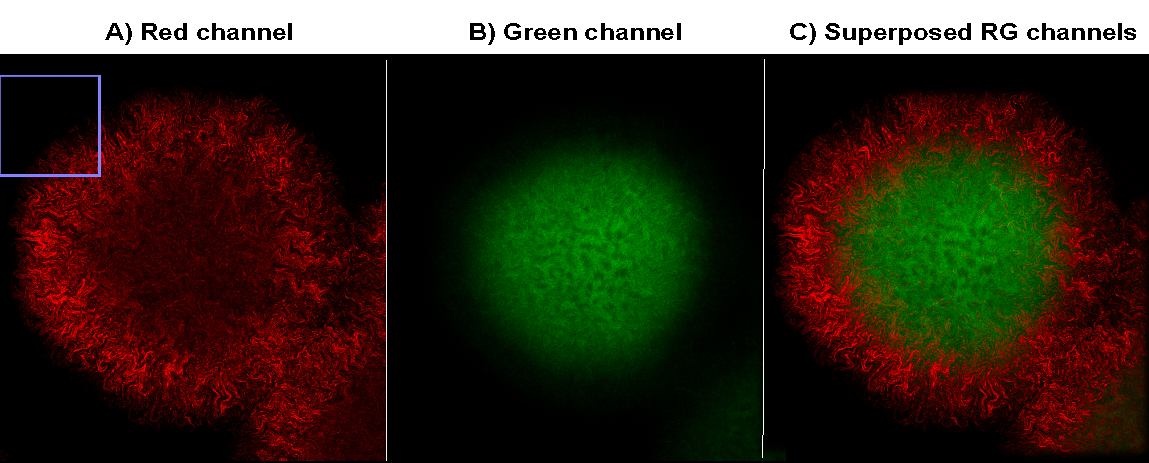
\includegraphics[width=1\textwidth]{chapters/Chapter 3/rgchannels}
    \caption{add}
    \label{rgchannels}
\end{figure}

To test the impact of aTc on the patterning of the circuit, we prepared the agar on the MaTek plates with different levels of aTc, ranging from 0 to $10^1 \mu M$.
Different colony patterns arise from this aTc walk as seen in Fig.~\ref{atcwalk_timeseries_confocal}A.
The colonies exhibiting more spatially heterogeneous behaviour are those with high aTc ($10^1 \mu M$).
This high aTc condition is further explored by imaging every day.
In Fig.~\ref{atcwalk_timeseries_confocal}B, we see how over time, the center of the colony oscillates from black to red to green.
As this happens, rings get added from the center as in~\cite{Konow2019}'s inner ring addition mechanism.
The final snapshot (64h) shows green, red, green, red progression steaming from the center.

\begin{figure}[H]

    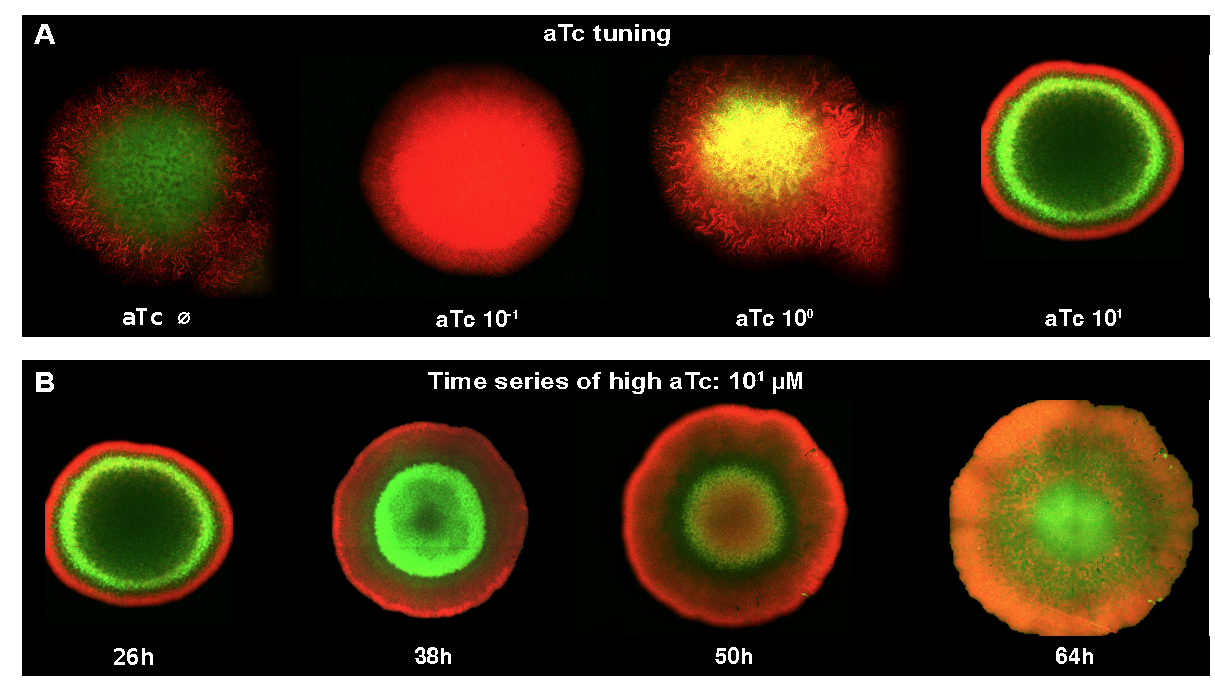
\includegraphics[width=1\textwidth]{chapters/Chapter 3/atcwalk_timeseries_confocal}
    \caption{\textbf{Confocal images of small colonies with gene circuit 3943}. A) Colonies with different atc conditions at time 26h: no aTc $10^{-1} \mu M,10^{0} \mu M,10^{1} \mu  $. B) Time series of single colony with high aTc condition ($10^1 \mu M$).}
    \label{atcwalk_timeseries_confocal}
\end{figure}

Following this work, we continued studying this synthetic patterning system more in depth.
Two routes were followed.
The first one involved specific shaped domains achieved by imprinting the agar with bacteria using shaped objects (Fig.~\ref{shmoo}).
The aim was to understand how the pattern adapts under different shaped domains.
The second route, and most explored, involved larger colonies to determine whether more repeats would form in a Turing-like behaviour.
This was achieved by carefully diluting the sample and plating a single colony without any neighbours.

\section{Modelling framework for synthetic circuit in bacterial tissues}
Most theoretical studies which involve Turing patterns, numerically simulate their system using square domains with no-flux or periodic boundary conditions.
However, these numerical domains are often not biologically realistic.
For exampled, the system we have developed experimentally involves more specific conditions including shaped domains, stochastic growth and absorbing boundary conditions.
To have a predictable model of our experimental system, the numerical solver had to be adapted to include such domain characteristics.

\subsection{Alternating Direction Implicit Method with defined domains}\label{Alternating Direction Implicit Method with defined domains}
All simulations in this chapter are performed in a \acrshort{2D} space to match the \acrshort{2D} focal plane captured by the confocal microscopy.
For this purpose, the numerical solver schema  \acrfull{ADI} is used.
This numerical solver produces a 2D space solution in time for the $n$ number of species of the model.
This method is chosen over \acrshort{CN} used in the previous chapter, as it is more efficient to solve 2D problems due to the matrix diagonalisation (see Section~\ref{numerical_methods}). More specific details of ADI can be found in Section~\ref{ADI}.



ADI is originally defined to solve square domains.
To integrate our specific domains with the solver, a masking system is used where a "shape matrix" is passed containing the shape of the domain.
The "shape matrix" has is a boolean matrix of $IxJ$ size which contains information on the location of the cells.
1's determine cells, while 0's determine agar.
When passing this matrix to the solver, the algorithm computes reaction and diffusion terms in 1 positions while it only computes diffusion in 0's.
Fig.~\ref{mask}~right shows the "shape matrix" where 1's are black and 0's are white.
Additionally, this figure shows what functions are computed in which regions.
How the "shape matrix" is defined depends on the experimental setup.
Using this masking method, we will obtain a solution for the $n$ number of species of our model, in time and in space, within the biofilm.

\begin{figure}[H]
    \centering

    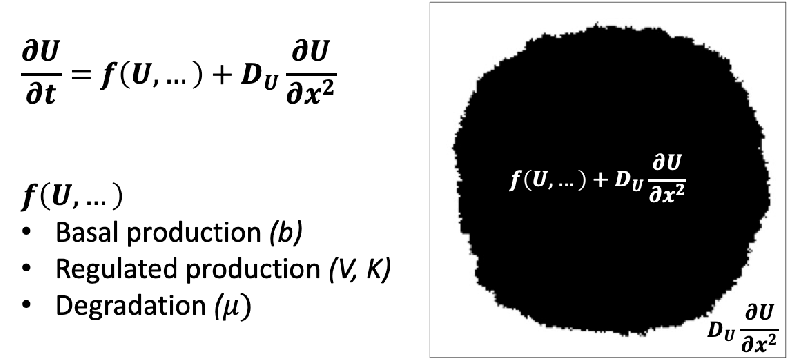
\includegraphics[width=0.9\textwidth]{chapters/Chapter 3/mask}
    \caption{a}
    \label{mask}
\end{figure}

\subsection{Static Shaped domains}
Following the small rings produced in this thesis, Tong Zhu from the Isalan Lab started experimenting with non-circular domains.
Specific shapes were obtained by imprinting the agar with bacteria using shaped objects.
Fig.~\ref{shmoo}A shows the resulting biofilm after impregnating the agar with bacteria using the edge of a glass coverslip. %TODO ref figure
In this thesis, the biofilm shape is replicated by using a "shape matrix" derived from the microscopy image Fig.~\ref{shmoo}B.
This is done through image recognition on the microscopy snapshots to detect areas with cells (see Section~\ref{Tissue area recognition}).


\begin{figure}[H]
    \centering

    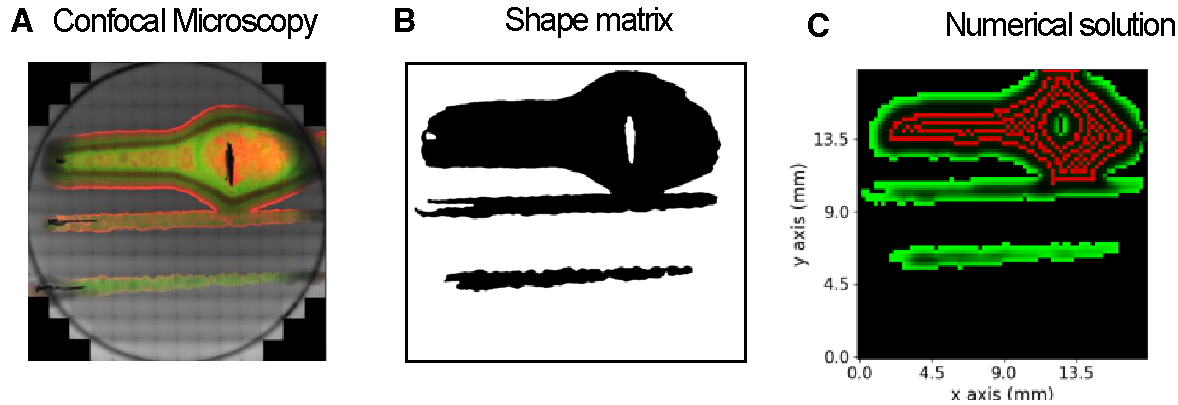
\includegraphics[width=1\textwidth]{chapters/Chapter 3/shmoo}
    \caption{}
    \label{shmoo}
\end{figure}
Using the masking method with ADI explained in ~\ref{Alternating Direction Implicit Method with defined domains}, a numerical solution was computed within the defined biofilm.
The PDE system used is the six-equation model (Eq.~\ref{[6 equation proteins]}), which describes synthetic circuit 3954, using a Turing parameter set found through linear stability analysis.
The numerical solution is shown in Fig.~\ref{shmoo}C as a superposition of the red and green channel.
Details on the plotting the numerical solution of the 6-equation as a red-green image like confocal microscopy can be found in Section~\ref{Plotting superposed numerical solution as confocal microscopy results}

\subsection{Growing colony with cellular automaton}
Most of the work we carried out experimentally to explore the system was done in bacterial colonies.
These colonies are radially growing biofilms with stochastic cell division.
Therefore, the static image recognition method used above is not suitable as we do not have time-series confocal data for most samples to create a dynamic "shape matrix".
To recreate the dynamic behaviour of the colony growing, a stochastic growth model was developed using a cellular automaton.

A cellular automaton is a discrete model of computation constructed with a few basic rules ~\parencite{gardner1970mathematical}, which can accurately describe how the shape of the bacterial colony evolves over time.
As the "shape matrix", the cellular automaton consists of a boolean 2-dimensional matrix, where grid-points can be in a cell (1) or agar (0) state.
This boolean matrix evolves over time when the following three rules are applied: If an cell (1) grid-point has any agar (0) neighbours, it will divide into the neighbouring agar (0) gridpoint with a probability $p_{d}$.
No cell death (1 to 0 transition) is permitted.
Newborn cells inherit the full concentration of their mother cells.
This last assumption is taken as mRNA transcript homeostasis ensures concentration of mRNAs is mantained at cell division and as cell size increases by scaling between transcription rates and cell size ~\parencite{berry2022mechanisms,volteras2023global}.
Because we are modelling protein concentration, we can then assume that mRNA concentration is linearly correlated with protein concentration for synthetic genes like ours.
If some dilution occurs, this can be accounted for in the degradation terms of the PDE model.

To model a single colony, a 0's matrix is initialised with a 1 in the middle, describing the first cell as it occurs in single cell colonies.
When the cellular automaton rules are applied to this initial matrix, a circular cell domain starts growing stochasticly, resembling a bacterial colony (see Fig.\ref{cas}A-B).
The division process consists of a probabilistic process where division occurs or not based on a probability of division ($p_{d}$).
The division process is iteratively applied to the matrix until the final time (T) is reached.
The computation is applied every ‘m’ hours, so
\begin{equation}
        T = \sum_{n=1}^{T/m} m\cdot n
\end{equation}

e.g. if $m=0.2$ at $T=0.2, 0.4, 0.6 \ldots etc$ .
The growth rate can be tuned by increasing the probability of division ($p_d$) or decreasing $m$, so it matches the experimental growth rates. Furthermore, different $p_d$’s can be applied to different regions of the matrix to achieve faster growing subregions within the colony (see Fig.~\ref{cas}C). Finally, to simulate two colonies, two 1’s are placed at a distance (see Fig.~\ref{cas}D).

\begin{figure}[H]
    \centering

    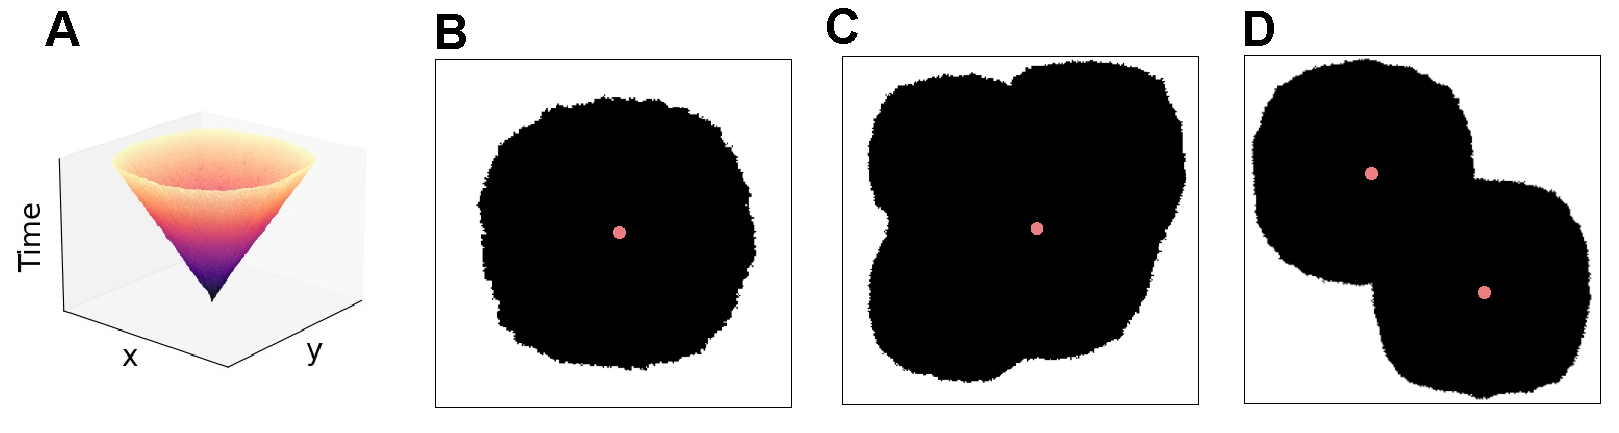
\includegraphics[width=1\textwidth]{chapters/Chapter 3/cas}
    \caption{}
    \label{cas}
\end{figure}

The masks obtained can be used to compute the solution of the PDE in the biofilm.
Unless otherwise stated, a reflective boundary condition (Neumann) is used at the edge of the square where the agar finishes.
Taking an arbitrary parameter set, this method produces a numerical result similar to that of the colonies obtained in Section~\ref{Rings in small colonies with high aTc}.
The comparison can be seen in Fig.~\ref{small colony experiment vs model} where the red edge with green center is reproduced.
This pattern is commonly seen throughout, as it stems from the boundary effects at the edge of the colony which is capture by the masking method.
At the edge of the colony, there is a depletion of diffusers as they leak out onto the agar.
By looking at the circuit (Fig.~\ref{fig:synthetic circuit_chapter2}), we can observe that diffusors are direct GFP activators and mCherry inhibitors.
Therefore, as they get depleted, red is produced and green decays.
\begin{figure}[H]
    \centering

    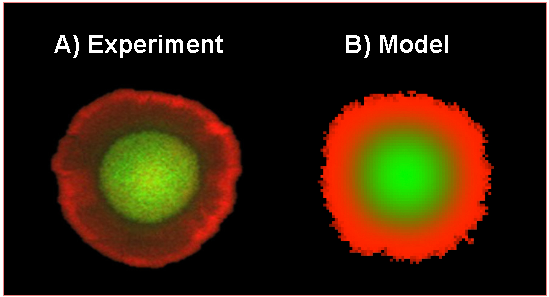
\includegraphics[width=0.6\textwidth]{chapters/Chapter 3/small colony experiment vs model}
    \caption{}
    \label{small colony experiment vs model}
\end{figure}

\subsection{Adapting time and space in the dimensionless model}
When solving our system numerically, time and space are key parameters that define the bounds of our simulation.
As seen in the previous chapter , time and space are dimensionless and dependent on the model’s parameters
\begin{equation}\label{time_space_transform}
    t = \frac{t*}{\mu _a}, \quad x = \sqrt{\frac{k_{1}D_{u}}{\mu_{a}\mu_{u}}}x^*
\end{equation}

In the parameter sampling used, $\mu_a = 0.3 \,h^{-1}, \,k_1 = 0.0183 \,h^{-1},\, \mu_u = 0.0225\, h^{-1}$ and $D_U$ is sampled from a range of $0.1-10 \,mm^2h^{-1}$.
Using Eq.~\ref{time_space_transform}, time is transformed so that $t^*=3.3\cdot t$.
Space is also transformed but is dependent on $D_U$, which is sampled from a range.
Therefore, for $D_U = [0.1, 10] \,mm^2 h^{-1}$, $x^* =[1.92 - 0.192] \cdot x$.
Using realistic exsperiment time and space, the following dimensionless values are obtained:
For time $t=166\,h$, dimensionless time $t^*=50$.
Dimensionless space  $x^*=16$ is taken so  $x = [8.32, 83.2] \,mm$, with $D_U = [0.1, 10]\, mm^2 h^{-1}$ respectively.
These values of t and x lie within realistic physical parameters for our system.
These transformations are dependent on parameters that may vary experimentally, and therefore some uncertainty must be allowed.
The experimental values used here are an example on how to carry out the transformations, however all simulation parameters for space and time can be found on TableX and Table Y.
%TODO add somewhere params of simulations in appendix to justify transfomations
\section{Colony pattern dynamics in parameter space searches}

The experimental work in this thesis produced the first rings observed in the system, where small colonies were used (Section~\ref{Rings in small colonies with high aTc}).
Following this, experiments were carried out in larger colonies by Dr.~Jure Tica, Tong Zhu and Dr.~Georg Wachter and Dr.~Dario Bazzoli from the Isalan Lab.
From here onwards, all experimental results were produced by them unless otherwise stated.
A wide variety of patterns were produced by growing larger colonies.


\subsection{Circuit exploration in literature-based distribution}
In parallel to microscopy work, the model predicted a wide variety of patterns could be produced in different dynamical regimes, which matched the experimental variability.
This was shown by exploring the parameter space of our circuit within literature-based ranges.
The distribution used is described in Section~\ref{Definition of parameter space based on literature parametrisation} and more specifically Table~\ref{tab:literature param distributions}.
In this exploration, first linear stability analysis was carried out and outputs were classified following linear stability classification in Fig.~\ref{fig:dispersions}.
The frequencies in parameter space of the linear stability solutions are shown in Fig.~\ref{system_class_frequencies}.
\begin{figure}[H]
    \centering

    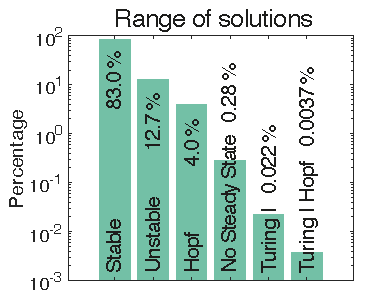
\includegraphics[width=0.6\textwidth]{chapters/Chapter 3/system_class_frequencies}
    \caption{The optimised parameters produce a wide variety of analytical solutions, expressed as percentages (Right). }
    \label{system_class_frequencies}
\end{figure}

Examples of different linear stability analysis outputs were solved numerically, masked by a growing colony obtained with the cellular automata algorithm.
The different final pattern snapshots and time-series can be seen in Fig~\ref{system_class_simulations}.
A wide variety of patterns and dynamics is observed including stationary rings, travelling waves, stationary and non-stationary spots, labyrinths and bistability wedges.
This global model analysis, with biologically relevant parameters, showed that our circuit can produce a broad range of spatial patterns, together with spatially homogenous solutions.
Overall, Turing I hopf and Turing I patterns are the most interesting heterogeneities due to their periodicity and stationarity.
However, they are not very robust ($0.022\%$ and $0.0037\%$ respectively).
On the other hand, Hopf solutions also produce interesting heterogeneities which are sometimes periodic, and seem to occur more robustly ($4\%$).
It is important to add that Turing I Hopf solutions seem to produce patterns more robustly in this chapter than in chapter 1. %TODO add maybe in discussion
All of patterns shown are single steady state systems so we can understand the individual and isolated behaviour of that dynamical system.
However some interesting multistable systems are present such as the Turing-Hopf-Unstable system shown in Fig.~\ref{comparison_colonies_model_vs_experiment} Rings \#1.
\begin{figure}[H]
    \centering

    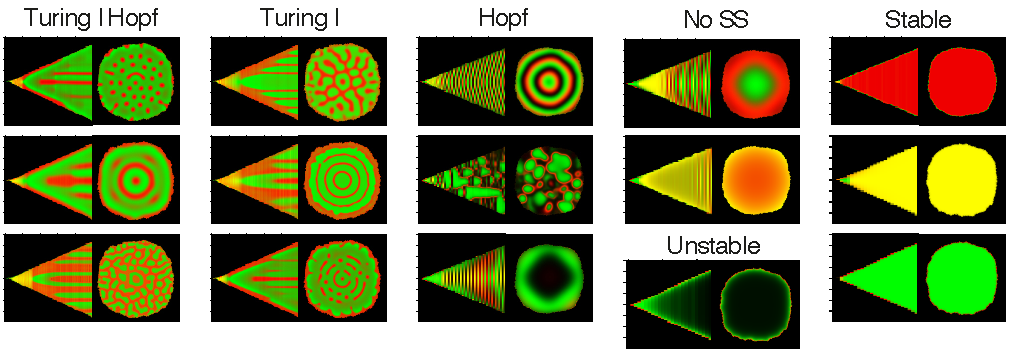
\includegraphics[width=1\textwidth]{chapters/Chapter 3/system_class_simulations}
    \caption{Simulations of the hybrid PDE-bacterial colony solver for all the types of analytical solutions of network \#1754. Kymograph (left) showing the timeseries of the cross-section and the final snapshot of the simulation (right). Green and red channels are superposed. }
    \label{system_class_simulations}
\end{figure}


This wide variety of patterns was explored, and corresponding experimental solutions were found (see Fig.~\ref{comparison_colonies_model_vs_experiment}).
As the model predicted, the system can experimentally produce rings, spots, wedges.
However, although labyrinths commonly appear in the model, they have not been found \textit{in-vitro}.


\begin{figure}[H]
    \centering

    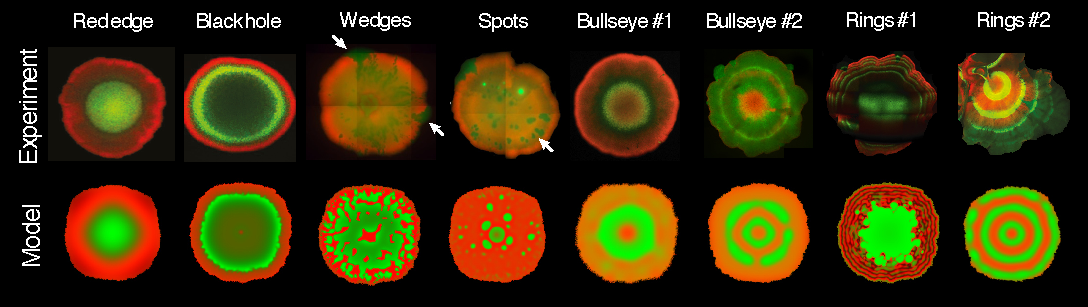
\includegraphics[width=1\textwidth]{chapters/Chapter 3/comparison_colonies_model_vs_experiment}
    \caption{Various spatial patterns are observed when the full circuit is tested in growing colonies in different experimental conditions (upper row). The white arrows show two wedges and a region of spot formation. Colony size and tuning conditions are listed in Table S1. Patterns are reproduced with the circuit model (bottom row); for parameters see Suppl. Info. 4. All images except Red Edge, Black Hole and Bullseye \#1 can be attributed to Dr.~Jure Tica, Tong Zhu and Dr.~Georg Wachter. }
    \label{comparison_colonies_model_vs_experiment}
\end{figure} %TODO add params and columns to appendix


\subsection{Circuit exploration in liquid-culture fits distribution}
In the previous section, the model was explored using large literature-based distributions and was compared to experiments in a different range of tuning conditions.
In this section we focus on a more constrained region of the parameter space obtained by fitting the model to liquid culture data (Section~\ref{Constrained parametrised distributions: fitting to liquid culture data of gene subcircuits}).
The aim of this parametrisation is to explore a model which is better linked to the experimental system in terms of parameters and behaviour.
More specifically, this constraining is carried out to prove that the obtained experimental patterns exist in this fitted parameter region, in particular the more Turing-like concentric rings (Fig.\ref{comparison_colonies_model_vs_experiment} Rings \#2).


In Section~\ref{Fitting process and the resulting best fit distributions.}, the model was fitted to dose response curves of subcircuits under high aTc and matched transfer functions conditions.
These are the same conditions where the Fig.\ref{comparison_colonies_model_vs_experiment} Rings \#2 appear.
As previously explained and shown in Fig.~\ref{fig:1d_distributions}, linear stability analysis was carried out on the fitted multivariate gaussian distribution with $q=10$, and 3 Turing parameter sets were found.
These are the closest 3 Turing parameter sets to the best fit solution.
Those three parameter sets were simulated using a colony growth mask (see Fig.~\ref{best_fit_colony_turing}). %TODO (see params in appendix)
Their dominant features, including a central circular green (Case \#1) or red (Case \#2) spot, surrounded by a ring of green fluorescence, and a wedge or labyrinthian like pattern.
These are all observed within the experimental data. %TODO ref experimental figure.

\begin{figure}[H]
    \centering

    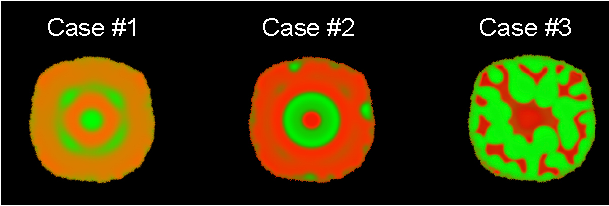
\includegraphics[width=1\textwidth]{chapters/Chapter 3/best_fit_colony_turing}
    \caption{ }
    \label{best_fit_colony_turing}
\end{figure} %TODO add params and columns to appendix

Although Case \#1 seems to have similar rings to the ones we are looking to replicate (seen in Fig.\ref{comparison_colonies_model_vs_experiment} Rings \#2), more rings would be needed to prove that the periodic ring like behaviour exists in the fit distribution.
Three routes can be taken to further explore the patterns present in the fit distribution.
The first one would be to tweak numerical parameters (e.g. space, time and growth rate) to obtain a different pattern.
However, numerical parameters are harder to explore from a computational parallelisation point of view.
The second one would be to sample more from the fit distribution to find more Turing parameters and simulate those.
However, Turing parameters are not commonly found and therefore it is also a computationally expensive task to obtain few results.
Finally, a third route exists which involves searching very closely around the vicinity of the already obtained parameter sets.
This route is chosen as it is the most efficient way of obtaining many Turing parameter sets that still belong to the fit distribution.

\subsection{Pattern exploration around the vicinity of Turing fit solutions}
The parameter space found around the fitted Turing parameter sets is explored, while keeping to the fit distributions. To do this, a small noise deviation is applied to the parameters with relative uncertainty of 1\%.
In other words, for each parameter $p$, a normal distribution is generated with mean $\mu=p$ and standard deviation $\sigma=p\cdot 0.01$.
This small noise perturbation to all parameters, which generates similar steady-state dose response behaviour, allows us to further explore the Turing parameter space near the best fit to the liquid culture.
For each value of uncertainty 2000 parameter combinations were analysed.
The Turing patterning robustness with different amounts of noise is shown in Fig.~\ref{fig:turing_fit_noise_robustness}A, showing how robustness decreases as more noise in the parameters is added.
This figure shows how the local parameter space around Turing conditions is highly enriched with patterns (e.g adding a relative uncertainty of 1\% around a Turing I solution produces 33\% Turing I solutions, whereas an uncertainty of 5\% produces 5\% Turing I solutions).
The average relative uncertainty in the Vm and Km parameters between biological repeats in liquid culture data of Fig. 1b was 4.8\%. This indicates that if a patterning region was found, Turing patterns could be sufficiently common to be reproduced.%TODO maybe add in discussion
The different analytical solutions for a relative uncertainty of 1\% are shown in Fig.~\ref{fig:turing_fit_noise_robustness}B, where we observe not only Turing I solutions, but also Turing I Hopf and Hopf solutions.
For this relative uncertainty (1\%), numerical solutions are computed and shown in Fig.~\ref{fig:turing_fit_noise_robustness}C.
Within the small vicinity of a ring-like Turing parameter set, we can find rings, spots and labyrinths.
In particular, we can find solutions with multiple concentric rings such as the one marked with an arrow in Fig.~\ref{fig:turing_fit_noise_robustness}C Case\#4.

\begin{figure}[H] % h! is a placement specifier; it tries to place the image here.
    \centering
    \begin{adjustbox}{center}
        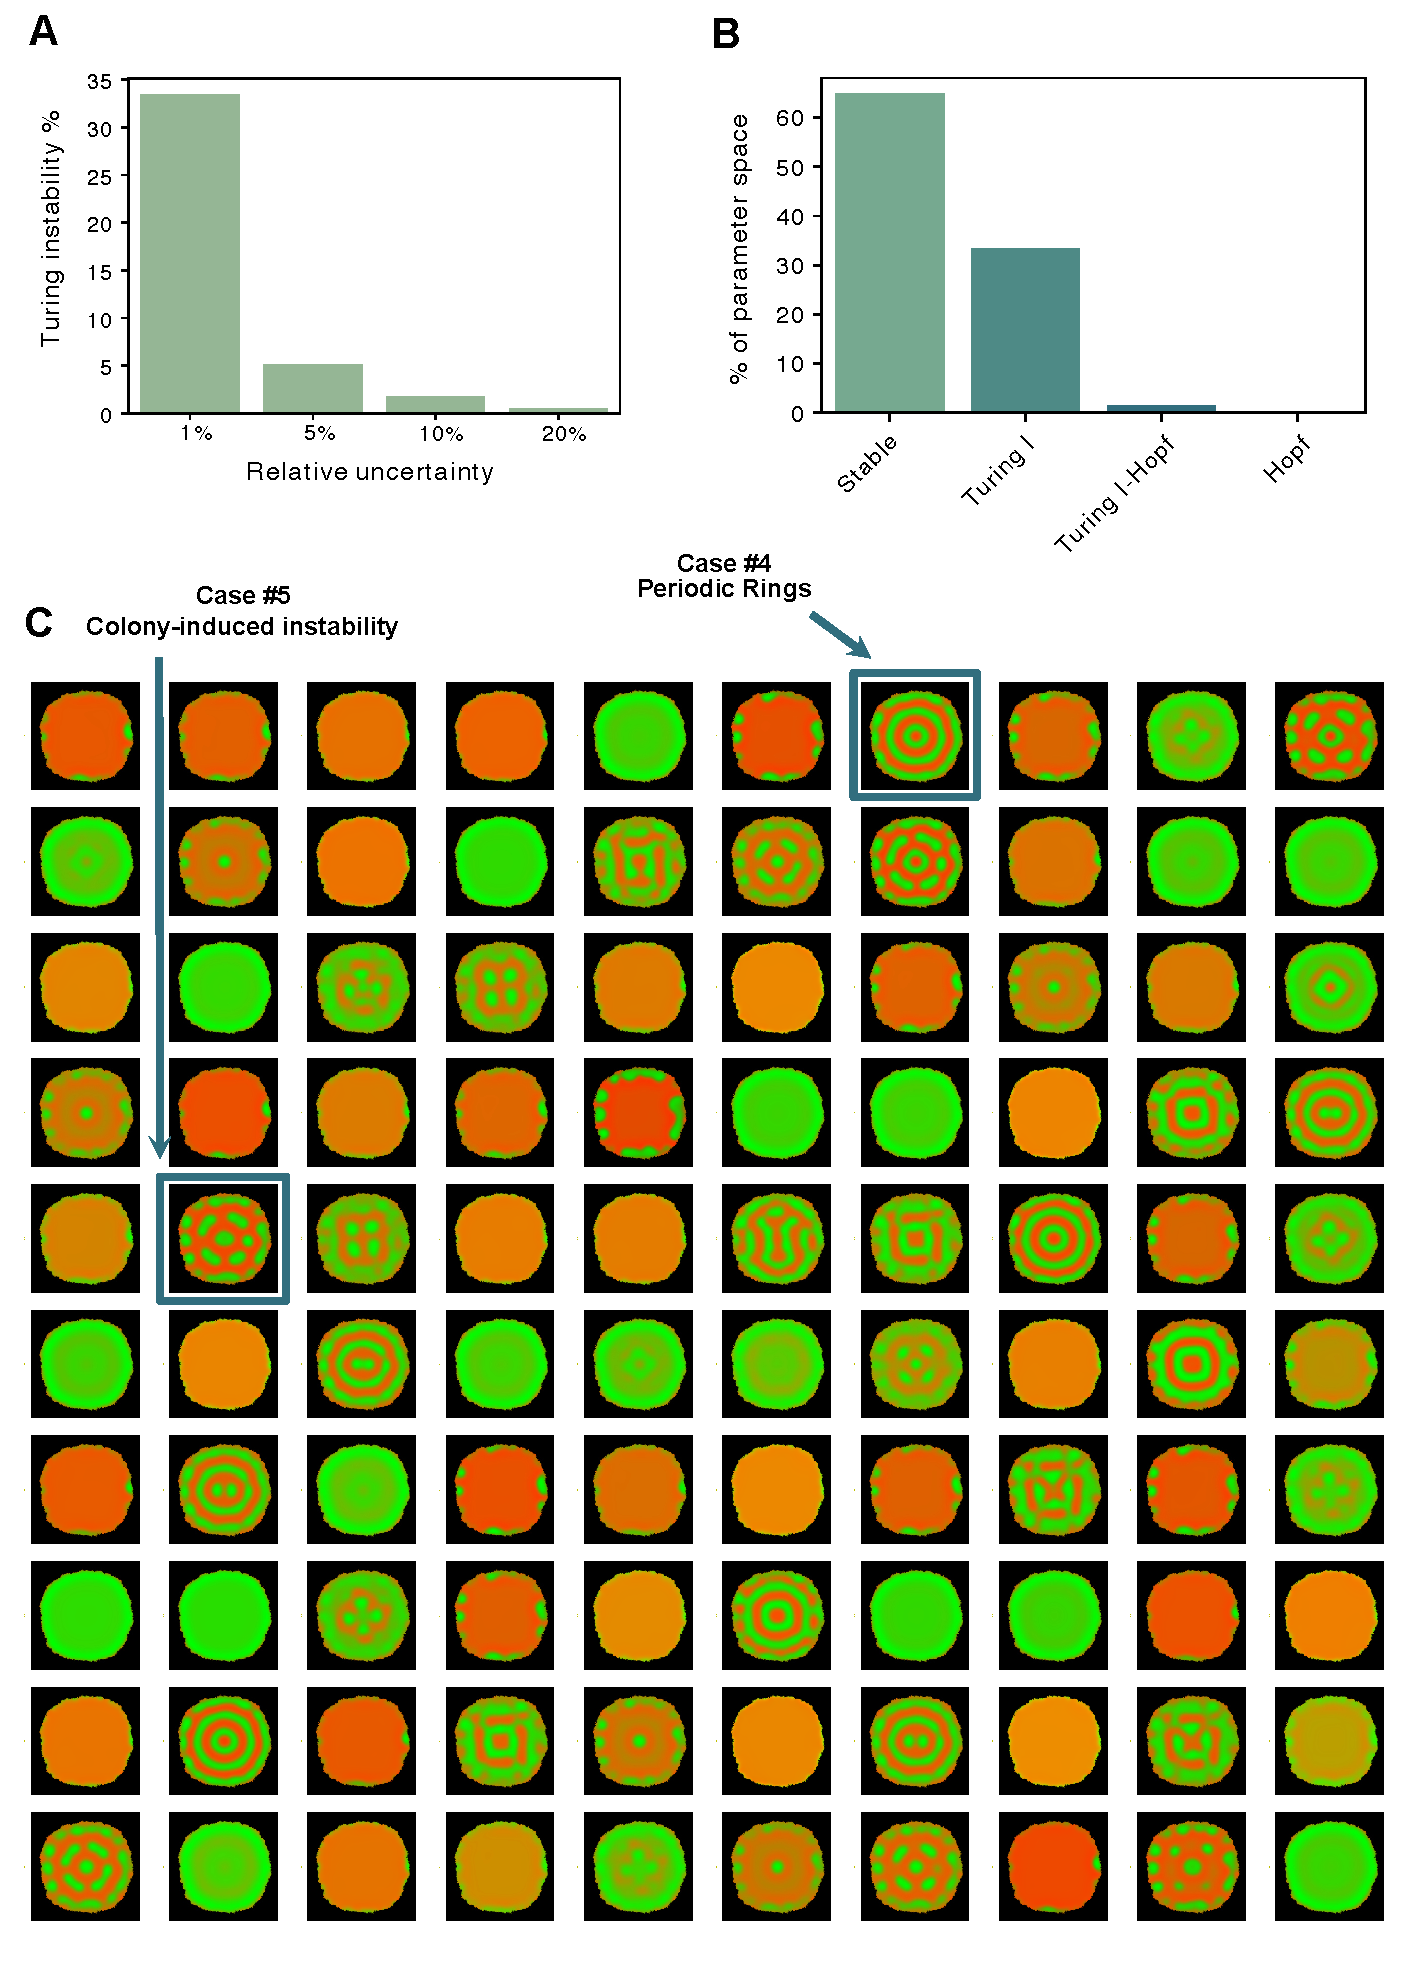
\includegraphics[width=1\textwidth]{chapters/Chapter 3/turing_fit_noise_robustness} % The name of your image file; assumes it is in the same directory as your .tex file
    \end{adjustbox}
    \caption{\textbf{Search around fitted Turing parameter set.} (A) Turing robustness with different levels of noise. (b) Using 1\% noise (mean $\mu=p$ and standard deviation $\sigma=p\cdot 0.01$), frequency of different analytical solutions: Simple stable 64.8\%, Turing I oscillatory 33.5\%, Turing I Hopf 1.5\%, Hopf 0.25\%. (c) Numerical simulations in growing colonies of 1\% noise distribution. Arrow points to Case \#4 which is a solution with multiple periodic rings}
    \label{fig:turing_fit_noise_robustness}
\end{figure}

Time series of this particular Case \#4 Turing solution is explored and compared to different snapshots of the bacterial colony patterns.
Outer ring addition dynamics of both the model colony and the experimental colony are shown in Fig.~\ref{fig:outer_ring_addition_modelvsexperiment}, where rings get added to the edge of the colony.
\begin{figure}[H] % h! is a placement specifier; it tries to place the image here.
    \centering
    \begin{adjustbox}{center}
        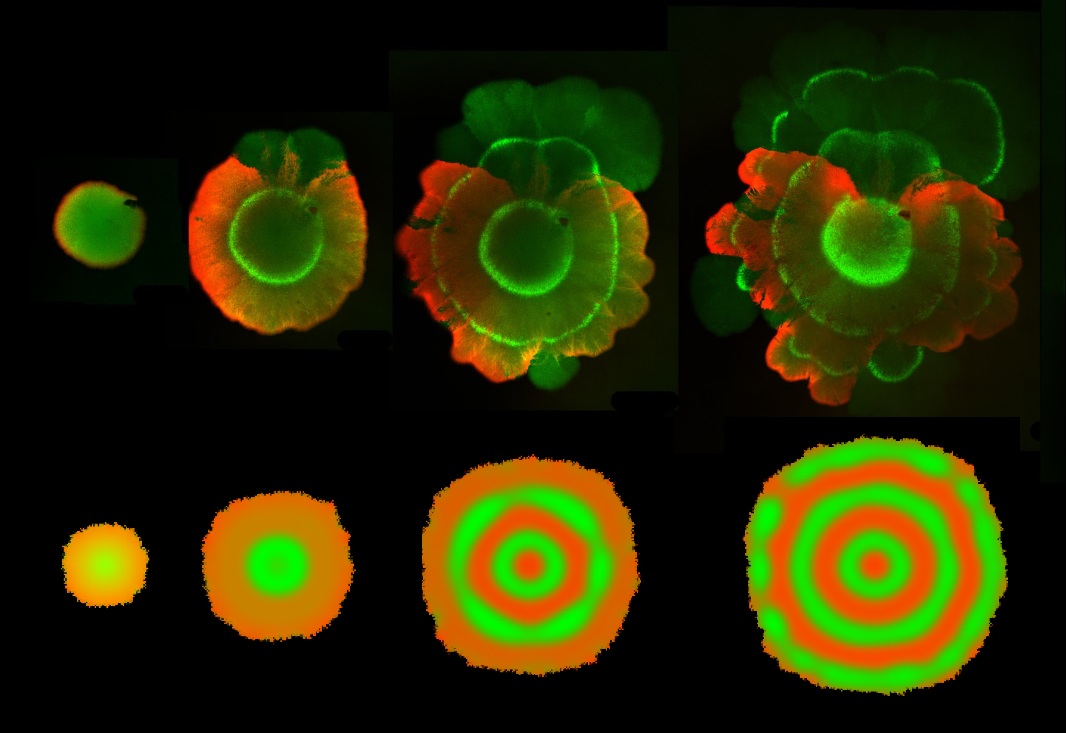
\includegraphics[width=1\textwidth]{chapters/Chapter 3/outer_ring_addition_modelvsexperiment} % The name of your image file; assumes it is in the same directory as your .tex file
    \end{adjustbox}
    \caption{\textbf{Search around fitted Turing parameter set.} (A) Turing robustness with different levels of noise. (b) Using 1\% noise (mean $\mu=p$ and standard deviation $\sigma=p\cdot 0.01$), frequency of different analytical solutions: Simple stable 64.8\%, Turing I oscillatory 33.5\%, Turing I Hopf 1.5\%, Hopf 0.25\%. (c) Numerical simulations in growing colonies of 1\% noise distribution. Arrow points to Case \#4 which is a solution with multiple periodic rings}
    \label{fig:outer_ring_addition_modelvsexperiment}
\end{figure}

Other interesting solutions are found such as the colony induced Turing pattern (Fig~\ref{fig:turing_fit_noise_robustness}C Case \#5).
In Fig.~\ref{fig:colony_induced_turing} we see an example of an instability induced by stochasticity in cell division or growth: the dispersion relation doesn’t show any unstable modes; however, the simulation shows a clear periodic heterogeneity.
The dominant mode of this dispersion relation (Fig.~\ref{fig:colony_induced_turing}A) has a wavenumber of 1.8, which corresponds to a wavelength of $2\pi/1.8=3.49$.
This approximately corresponds to the wavelength of the produced pattern (Fig.~\ref{fig:colony_induced_turing}B), meaning this stable mode has been excited to unstable and resulted in a Turing pattern.


\begin{figure}[H] % h! is a placement specifier; it tries to place the image here.
    \centering
    \begin{adjustbox}{center}
        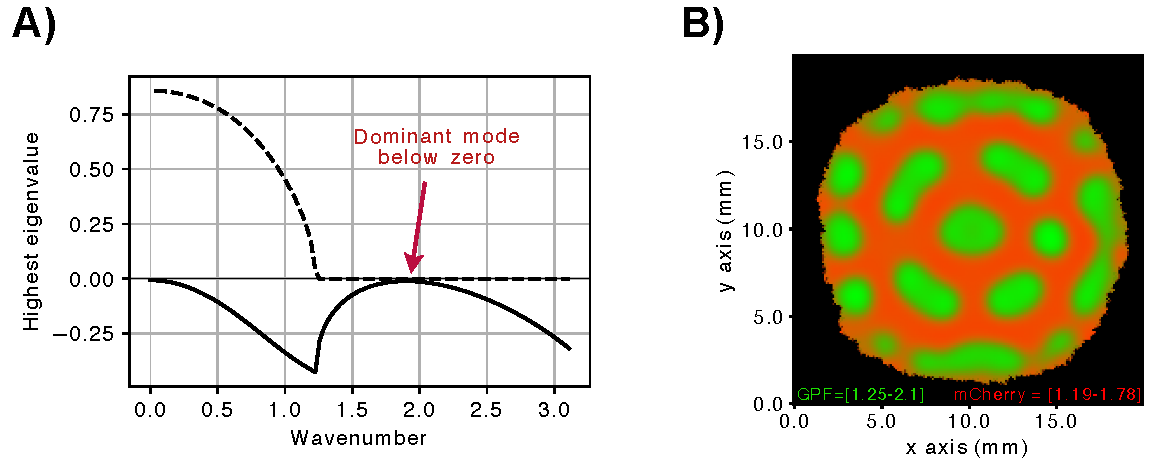
\includegraphics[width=1\textwidth]{chapters/Chapter 3/colony_induced_turing} % The name of your image file; assumes it is in the same directory as your .tex file
    \end{adjustbox}
    \caption{\textbf{Colony induced instability.}  (a) Dispersion relation showing a stable system. The most dominant mode (wavenumber=1.8, wavelength=3.49). (b) Regular pattern in numerical solution of stable system with dominant mode just below zero.}
    \label{fig:colony_induced_turing}
\end{figure}
%TODO discussion: histogram shows little robustness, but could be higher as stable systems sometimes display patterns in the vicinity of a Turing as they are almost stable.


\section{Elucidating mechanisms through experiment controls}
Although the patterns obtained experimentally might seem qualitatively similar to Turing solutions in bacterial colonies, further controls are needed to strenthen the hypothesis that these are Turing patterns.
Such controls involve introducing a perturbation in the model, which leads to a change in pattern features; and obtaining the same change in pattern when producing such perturbation experimentally.

Most of these perturbations except the deletions section will be applied to the Case \#4 Turing condition shown in Fig~\ref{fig:outer_ring_addition_modelvsexperiment}, where multiple rings appear using parameters from the fit distribution.

\subsection{Irregular growth}
The first control involves studying the pattern under different sizes of biofilm.
An interesting way to look at this problem is by understanding how the pattern changes within the same colony in smaller or larger areas.
By tuning the growth rates of the cellular automata differently in different regions of the colony, we can obtain faster growing domains which will be larger than others (see Fig.~\ref{cas}C).
This resembles the bacterial colonies produced which have faster growing edges.
The model shows that larger domains will produce more rings than shorter domains (see Fig.~\ref{fig:irregular growth} right).
This prediction is correct, as experimental data produces the same behaviour  (see Fig.~\ref{fig:irregular growth} left).
Additionally, in both model and experiment, this irregular growth leads to discontinuity in the concentric rings.
\begin{figure}[H] % h! is a placement specifier; it tries to place the image here.
    \centering
    \begin{adjustbox}{center}
        \includegraphics[width=1\textwidth]{chapters/Chapter 3/irregular growth} % The name of your image file; assumes it is in the same directory as your .tex file
    \end{adjustbox}
    \caption{\textbf{Effects of irregular growth in pattern.} }
    \label{fig:irregular growth}
\end{figure}


\subsection{Boundary effects}
The second control involves studying how boundary conditions might affect the resulting pattern.
The boundary conditions at the edge of the colony are always assumed to be absorbing boundary conditions because the diffusers produced in the biofilm get absorbed by the empty agar because of diffusion.
This boundary is indirectly encoded with the masking process (Fig.~\ref{mask}).
However, the boundary at the edge of the simulation square or in other words, where the agar would finish, has to be defined in the ADI numerical solver.
As in chapter X, the absorbing boundaries are introduced by using a Dirilichet boundary condition where the concentration at the boundary is zero $u=0$ as opposed to the previously used Neumann boundaries where the derivative at the boundary is zero.
More details on the encoding of boundaries can be found in Section~\ref{numerical_methods}.
Up to now, all simulations in this Chapter were computed using reflective boundary conditions at the edge of the square.
Here, we introduce absorbing boundary conditions and see that this perturbation leads to fewer rings being produced.
The hypothesis that absorbing boundary conditions make weaker patterns is then tested experimentally.
Absorbing and Reflecting experimental boundaries can be introduced using different sizes of agar plates where the colony grows.
A larger plate will resemble an absorbing boundary conditions as we assume diffusers build-up will be less prominent and there will always be a diffuser flux towards the edges of the plate.
On the other hand, a small plate will lead to the quick accumulation of diffuser and therefore these will quickly be reflected as they reach the boundary. %TODO maybe explain better
Experimental colonies behave according to model predictions, displaying fewer rings when grown in bigger plates.
%For a small agar plate, we define reflecting boundaries while for a larger plate we assume absorbing boundary conditions.


\begin{figure}[H] % h! is a placement specifier; it tries to place the image here.
    \centering
    \begin{adjustbox}{center}
        \includegraphics[width=1\textwidth]{chapters/Chapter 3/boundary_conditions_colony} % The name of your image file; assumes it is in the same directory as your .tex file
    \end{adjustbox}
    \caption{\textbf{Effects of boundaries.} The boundary condition affects the patterns. Multiple rings form when cells are grown in smaller wells (closed boundary), whereas fewer rings form when grown in larger dishes (open boundary). \TODO{change images with OG}s}
    \label{fig:boundary_conditions_colony}
\end{figure}

\subsection{Node deletions}
Another important perturbation is deleting nodes of the circuit to study how patterning is affected.
Deletions of each node described in Fig.~\ref{fig:deletion_circuits} were studied using analytical and numerical methods, by re-sampling the parameter space with the literature-based distribution.
The models were defined by taking the original six equation model and removing the following species: RpaI and TetR for Node A deletion, cinI for node B deletion and cI* for node C deletion (see Fig.~\ref{fig:deletion_circuits}).

\begin{figure}[H] % h! is a placement specifier; it tries to place the image here.
    \centering
    \begin{adjustbox}{center}
        \includegraphics[width=1.1\textwidth]{chapters/Chapter 3/deletion_circuits} % The name of your image file; assumes it is in the same directory as your .tex file
    \end{adjustbox}
    \caption{}
    \label{fig:deletion_circuits}
\end{figure}

No Turing I or Turing I Hopf instabilities were found when sampling these three circuits using linear stability analysis. %TODO mention how many.
Fewer samples were simulated using numerical methods and no patterns were observed either. %TODO specify what is a pattern
%TODO look into results in model
Therefore, the model predicts no patterns should arise from the node deletion variants shown in Fig.~\ref{fig:deletion_circuits}.

These variants were then built experimentally and tested by the
Isalan group.
Deletions for node A and node B involve removing the plasmid encoding for that node as in the model.
Deletion for node B involved deleting cinI which is the enzyme producing $OC_{14}$, therefore disconnecting node B from the circuit.
In this variant, node C is deleted too as its only feedback on the circuit is on cinI.
Thin green stripes in the GFP channel, similar to those of the full circuit in Fig.~\ref{fig:outer_ring_addition_modelvsexperiment} , were observed with the three controls after imaging the circuit daily.
Interestingly, the stripes consistently coincided with the outline of the colony at the previous timepoint (Fig.~\ref{fig:experimental_node_dele}).

\begin{figure}[H] % h! is a placement specifier; it tries to place the image here.
    \centering
    \begin{adjustbox}{center}
        \includegraphics[width=1.1\textwidth]{chapters/Chapter 3/experimental_node_dele} % The name of your image file; assumes it is in the same directory as your .tex file
    \end{adjustbox}
    \caption{Control experiments testing circuit deletions. All images are taken 4 days after plating, and only the GFP channel is shown. Controls are node A deletion, node C deletion and cinI-nodeC deletion.}
    \label{fig:experimental_node_dele}
\end{figure}

In this control, the model and experiments disagree as the model does not predict the ring patterns appearing experimentally.
Therefore, these specific rings in the controls cannot be explained with the Turing mechanism and other mechanisms need to be explored.
This suggested that stripe formation was induced by the imaging procedure, possibly because of the drop in temperature during the imaging.
\subsection{Temperature variations}
A potential explanation for the rings is that stripe formation was induced by the imaging procedure, possibly because of the drop in temperature during the imaging.
This hypothesis was not tested with the model because of lack of time.
However, it was explored experimentally by Dr.~Jure Tica and Dr.~Dario Bazzoli and will be shown here for story completeness.

Different imaging frequencies were used to understand how the pattern is affected by the imaging procedure.
First, they imaged the colony every day for 5 days and 4 rings appeared.
Then, they only imaged on day 1 and day 4 after plating and this lead to 3 rings (see Fig.~\ref{fig:cold_shock_experiments}left).
Finally, imaging was only done on day 4 and no rings appeared as seen in Fig.~\ref{fig:cold_shock_experiments}center, right.
Overall, imaging everyday is not required for periodic patterning.
However, it is required to image in day 1 to get periodic stripes.



\begin{figure}[H] % h! is a placement specifier; it tries to place the image here.
    \centering
    \begin{adjustbox}{center}
        \includegraphics[width=1.1\textwidth]{chapters/Chapter 3/cold_shock_experiments} % The name of your image file; assumes it is in the same directory as your .tex file
    \end{adjustbox}
    \caption{The bottom row shows the effects of cold shock, where the first colony is exposed to cold shock 1 day after plating, whereas the other two colonies are not. In the first colony the first stripe is a result of the cold shock, whereas the other stripes form at a constant temperature of 37 °C. \TODO{modify label, modify image}}
    \label{fig:cold_shock_experiments}
\end{figure}

To avoid the cold shock effect caused by the imaging procedure, we sought to keep the cells at a constant temperature while imaging.
Colonies were grown for a day and then transferred to the microscope.
The cells were kept at 37°C with a stage-top incubator, and images were taken every hour.
Consistent with the cold shock hypothesis, the first stripe formed soon after the start of the imaging.
Surprisingly, additional stripes formed on the edge of the colony, in parts of the colony with the most prominent outgrowth (Fig.~\ref{fig:microscopy_timeseries}).
Both the timelapse (Fig.~\ref{fig:microscopy_timeseries}) and day1-day4 imaging (Fig.~\ref{fig:cold_shock_experiments}center) show stripes without everyday imaging.
This suggests that after the first stripe is seeded additional stripes can form in a circuit-dependent, reaction-diffusion process.


\begin{figure}[H] % h! is a placement specifier; it tries to place the image here.
    \centering
    \begin{adjustbox}{center}
        \includegraphics[width=1.1\textwidth]{chapters/Chapter 3/microscopy_timeseries} % The name of your image file; assumes it is in the same directory as your .tex file
    \end{adjustbox}
    \caption{GFP fluorescence was imaged over 60 hours at constant temperature 37 °C. Imaging began after the colony had grown for 24 hours. A) The image of the final timepoint shows three stripes in the top right corner of the colony where growth is most prominent (3), only a single stripe forms at the bottom where there is less growth (1). B) Plot of the fluorescence along the white slanted line in the micrograph with moving average smoothing. C) The spatiotemporal profile of GFP evolution shows that the stripes form at the edge of the colony. After an initial burst of fluorescence, the signal decreases over time.}
    \label{fig:microscopy_timeseries}
\end{figure}

\subsection{Different growth rates}

%TODO comment on how would you test: changing Vm parameter for cold shock. Starting simulation with prepattern. proof of robustness of Turing patterns?
%TODO discussion: Pcin promoter seems to be sensitive to cold and that allows seeding of prepattern.
\section{Discussion}
\begin{itemize}
    \item Rings are produced by circuit
    \item Model can replicate all patterns using Turing params
    \item Using parametrised, we can also replicate rings
    \item Wide variety of patterns can be produce in small vicinity
    \item circuit extremely senstivite not only to params but also to growth rates.
    \item Growth induced patterns
    \item some controls point that model is correct such as boundary controls or irregular growth
    \item however deletion controls contradict model, making Turing not clear
    \item temperature shocks can produce patterns but periodic patterns can be obtained with single temperature shock ... prepatterns add robustness?

\end{itemize}
%%TODO summary chapter2
%%TODO commdent on diffusion constant matching between experiment and model


%\section{Modelling bacterial colonies}
%\subsection{openboundary circle shape growth noise}
%\section{Explore patterning potential}
%\subsection{general params}
%\subsection{parametrised params}

    \chapter{Methods}
\section{Finding the steady states: Newton-Raphson method}\label{newton_raphson}

To obtain the roots of the system, the Newton-Raphson algorithm was implemented.
The Newton-Raphson algorithm, also known as Newton's method, is a numerical technique for finding approximate roots of a real-valued function. It starts with an initial guess, which is then refined through iterations. In each iteration, the method uses the current approximation to find a better one, applying the formula
\begin{equation}
x_{n+1} = x_{n} - \frac{f(x_{n})}{f'(x_{n})}
\end{equation}

where $f(x)$ is the function and $f'(x)$ its derivative.

This algorithm was implemented in python using a tolerance value of 0.000001 and a maximum of 15 iterations after which the algorithm stopped searching for a root.
Because the system had the potential for multi-stability, several initial conditions need to be searched to obtain all steady states.
In total 100 initial conditions were analysed by the Newton-Raphson to obtain all the roots of the system.
The 100 conditions were chosen performing latin-hypercube sampling of a n dimensional space (n being the number of species), from a uniform distribution with a range from $10^{-3}$ and $10^3$ .
%Approximately, the root finding for a single parameter set takes around 2 seconds.
\section{Sampling method}\label{sampling method}
If no parameters from a system are known, sampling of the whole parameter space must be done to understand the system's behaviour.
Different methods exist for sampling parameter spaces.
Several studies have shown that latin-hypercube sampling (LHS) has a higher efficiency than grid sampling or random sampling when searching through high dimensional spaces.
The efficiency over grid sampling might be explained because not all dimensions of the model are important, meaning some parameters might be sloppy.
Therefore, not all parameters have to be explored thoroughly as done in grid sampling~\parencite{Iman2014, Bergstra2012}.
The three sampling regimes are shown in Fig.~\ref{distributions}A.

In LHS, a distribution and a number of desired samples is given as an input.
The algorithm then divides the space sections according to the distribution given (e.g in a normal distribution, more sections will appear near the mean value).
Then, one sample is positioned randomly somewhere in each section.
For a 2 dimensional parameter space, no samples can be in the same column or row.
This can be scaled up to high multidimensional spaces. %TODO replace gaussian, gaussian, uniform. find original powerpoints
The LHS scheme is shown in Fig.~\ref{distributions}B.
\begin{figure}[H]

    \includegraphics[width=1\textwidth]{chapters/Methods/distributions}
    \caption{\textbf{Sampling method for high dimensional spaces}. \textbf{(A)} Types of potential sampling methods. \textbf{(B)} Latin-Hypercube sampling with uniform distribution for a 2 dimensional parameter space. Space is separated in 5 sections for each parameter, leading to 5 samples (red dot). No sample is present in the same row or column. \textbf{(C)} Parameter distributions used for Latin-hypersube sampling. The 4 different types of parameters have different distributions depending on the ranges defined. All of them are uniform distributions in log-scale. }
    \label{distributions}
\end{figure}
The distribution given as an input to the LHS algorithm, will be the resulting distribution of your samples. For the purpose of this search, the distributions chosen are uniform distributions in a logarithmic scale (log-uniform distribution). The uniform distribution, although it does not describe many phenomena in biology, can be useful when no prior knowledge is known about the parameters~\parencite{Frank2009}. The logarithmic component is used to make sure parameters from all scales are represented equally, instead of having a higher frequency of values from larger scales. Log-normal distributions are commonly used for modelling in biology, however due to the nonexistent prior knowledge on our parameter values, the log-uniform is used instead. The log-uniform distribution is defined within a certain range, which varies depending on the parameter type. The distributions for each parameter type are shown in Figure 20c. Overall, 1 million samples where produced using the LHS with a uniform distribution in log-scale. All parameters except the diffusion rates ($d$) and the cooperativity ($n$) where sampled using LHS and the distributions shown in Figure 20c.



\section{Dispersion peak height optimisation: Adapted random walk Metropolis}
In this section, the optimization of the dispersion peak height using an adapted random walk-Metropolis (RWM) algorithm will be explained.
The RWM algorithm is a common type of Markov Chain Monte Carlo (MCMC) method that uses a Metropolis Algorithm.
The RWM algorithm is used for sampling a variable to understand its probability distribution, without getting stuck in local maxima.
This algorithm is used in a Bayesian context when trying to fit a model with parameters $\theta$ to data $D$.
A probability distribution is obtained, which suggest what parameters $\theta$ are better to represent the data $D$.
However, in this case, the aim is not to fit a model to any data $D$, but to maximise the dispersion peak height.
Therefore, a variant of the RWM algorithm will be developed as shown in Fig.~\ref{Simulated Annealing}.

\begin{figure}[H]
    \centering
    \includegraphics[width=1\textwidth]{chapters/Methods/Simulated Annealing}
    \caption{\textbf{Adapted random walk-Metropolis algorithm workflow}.  }
    \label{Simulated Annealing}
\end{figure}
The starting point of the algorithm is to propose a Turing parameter set which will be the starting parameter set to be optimized in the process.
From that parameter set, a new parameter set is proposed where all parameters are varied slightly.
The variation is chosen randomly from a uniform distribution around the parameter value. The uniform distribution is defined as $U(X_{0} - X_{0}T, X_{0} + X_{0}T)$, where $X_{0}$ is the initial parameter to be varied and T is a temperature constant that will define the amount of variation to be applied. In this case, $T=0.1$. So if $X_{0}=100$, the uniform distribution is U(90,110).
This step is done for all parameters of the parameter set at every iteration, producing a new parameter set $X_{1}$.
The Markov Chain component is present because the step taken is only dependent on the current state, and not on information prior to that.
The Monte Carlo is due to the randomness involved in choosing the new parameter set.
In the normal RWM algorithm, the posterior of $X_{0}$ and $X_{1}$ are compared to see which parameter set is a better fit to the data $D$.
However, for the purpose of optimizing dispersion, the posterior is neither available nor relevant.
Instead the dispersion peak height value is used.
Once the new step $X_{1}$ is taken, the dispersion peak height ($d_{X_{1}}$) is calculated and compared to the dispersion peak height  of $X_{0}$ ($d_{X_{0}}$). If the dispersion peak height has improved, $d_{X_{1}} > d_{X_{0}}$, the move is accepted and $X_{1}$ becomes $X_{0}$.
If no improvement has been made, $d_{X_{1}} < d_{X_{0}}$, the Metropolis algorithm comes in to place: The ratio of the dispersions is calculated, $r = \frac{d_{X_{1}}}{d_{X_{0}}}$  and compared to a normal distribution $N(1,0.001)$.
If the ratio is higher than a random number from the distribution $N(1,0.001)$, the move is accepted and $X_{1}$ becomes $X_{0}$.
Otherwise, the move is rejected.
This ensures that big decreases in the dispersion peak height ($r \ll 1$) are not accepted while small decreases ($r \approx 1$)  are accepted.
Usually, the RWM uses a distribution $U(0,1)$ for this step.
An optimization with this distribution was attempted, resulting in no significant improvement of the dispersion peak height.
Therefore, the variant of the $N(1,0.001) $ was introduced to ensure a more strict regime is in place, hence reducing the number of accepted negative steps.


\section{Numerical solution by finite-difference methods}
Obtaining a solution for a system of equations can become a complex problem if working with a system of large system of non-linear PDEs.
Because an analytical expression for the solution is almost impossible to obtain, finite-difference methods are used for cases like this one.
Finite-difference methods consists in discretising space and time to approximate the PDE system to a system of algebraic equations that can be easily solved by matrix algebra techniques~\parencite{Morton1994}.
By discretising time and space, the two independent variables can be expressed as:
\begin{subequations}
    \begin{equation}
        t_{n} = n \cdot \Delta t, \quad n=0,\dots,N-1
    \end{equation}
    \begin{equation}
        x_{j} = j \cdot \Delta x, \quad j=0, \dots,J-1
    \end{equation}
\end{subequations}
While $\Delta t$ and $\Delta x$ are the time steps and the space steps respectively, N and J are the number of discrete time and space points in our grid.
$\Delta t$ and $\Delta x$ can be defined as $ \Delta t = \frac{T}{N}$ and $\Delta x= \frac{L}{J}$ respectively where T and L are the final time and space values in the grid.
The aim is to derive a numerical solution that is approximates to the unknown analytical solution so $U(j\Delta x, n\Delta t)\approx u( j\Delta x, n\Delta t)$, where $U$ is the analytical solution and $u$ is the numerical solution.

When working with a numerical solver, the solver can perturb the systems behaviour due to the effects of the time-step, the integration method or the computer arithmetic.
When choosing a scheme to numerically solve a PDE, three different characteristics of the scheme need to be considered: Consistency, stability and convergence.
Firstly, for a scheme to be consistent, the truncation error must be reduced as $\Delta t \rightarrow 0$ or/and if $\Delta x \rightarrow 0$.
The truncation error is the resultant from using a simple approximation to represent an exact mathematical formula.
Secondly, the numerical method is said to be stable if the error (truncation or round-off) is not magnified as the number of time steps tends to infinity.
Finally, as the Lax equivalence theorem states, the scheme is said to be convergent if both consistency and stability are fulfilled.
This means that at any fixed point, if  time and space discretisations tend to zero, the numerical solution will tend towards the exact solution \parencite{smith1985numerical}.
The methods chosen to solve this system of equations are \acrfull{CN} for 1 dimension in space and \acrfull{ADI} for 2 dimensions. These methods are chosen because they are both unconditionally stable as shown by von Neumann stability analysis \parencite{strikwerda2004finite}. The unconditional stability is important to allow for larger $\Delta t$ and $\Delta x$, without getting an amplification of the error. Larger $\Delta t$ and $\Delta x$ will result in reduced computationally power. Although \acrshort{CN} is less computationally expensive than \acrshort{ADI}, it becomes extremely complex when scaled up to multiple dimensions. On the other hand, \acrshort{ADI} has a simpler structure in 2 dimensions that can be solved easily using the tridiagonal matrix algorithm. Hence, \acrshort{CN} is used to obtain 1D space solutions while \acrshort{ADI} is used for 2D.
%\begin{figure}[H]
%    \includegraphics[width=0.8\textwidth,center]{Methods/stencils.png}
%    \caption{\textbf{Stencils for numerical solution}.  A stencil is a geometric representation with nodes and edges, that represents the points of interest for the numerical approximation. The points of interest, which are the ones present in the equations, are shown in green. j and n are the current space and time points. \textbf{(A)} \acrlong{CN} stencil used in 1D numerical simulations. The axis are time and space ($x$). \textbf{(B)} \acrshort{ADI} stencil used in 2D numerical simulations. The axis are time and 2 dimensional space ($x$,$y$).}
%\end{figure}
\subsubsection{\acrlong{CN} method}\label{cranknicolson}
Consider a reaction diffusion system with one space dimension and boundary conditions
\begin{equation}
    \frac{\delta u}{\delta t} =  f(u) + D\pdvn{2}{u}{x},   \quad \quad \quad \quad \quad \quad \pdv{u}{x}\biggr\rvert_{x=0,L}=0
\end{equation}
The spatial part of the equation can be approximated to
\begin{equation}
    \\pdvn{2}{u}{x} \biggr\rvert_{x=j\Delta x,t=n\Delta t} \approx \frac{1}{2\Delta x^{2}}\left( U^{n}_{j+1} -  2U^{n}_{j} + U^{n}_{j-1} + U^{n+1}_{j+1} - 2U^{n+1}_{j} + U^{n+1}_{j-1}\right),
\end{equation}
while the production function can be approximated to $f ( U^{n}_{j})$.  The approximations can be better visualised using the \acrshort{CN} stencil (See Figure 19a). Applying \acrshort{CN}'s stencil to the grid point (i,j), the reaction-diffusion system can be expressed as

\begin{equation}
    \frac{U^{n+1}_{j} - U^{n}_{j} }{\Delta t} = \frac{D}{2\Delta x^{2}}\left( U^{n}_{j+1} -  2U^{n}_{j} + U^{n}_{j-1} + U^{n+1}_{j+1} - 2U^{n+1}_{j} + U^{n+1}_{j-1}\right) +  f( U^{n}_{j})
\end{equation}
By reordering this approximation into a linear equation, the resulting problem is defined by a simple linear equation containing matrices A and B. Where $\textbf{U}^{n+1} = [U^{n}_{0}, ... , U^{n}_{J-1}]$, the simplified system can be expressed as:
\begin{equation}
    \textbf{U}^{n+1} = A^{-1}(B\textbf{U}^{n} + f^{n})
\end{equation}
This method simplifies the complex system into a linear system that can be solved numerically. The solution given will be a 1 dimensional in space solution of the reaction-diffusion system. Although the method is  unconditionally stable, the solution can contain oscillations if $ \frac{\Delta t}{\Delta x^{2}} >\frac{1}{2} $ \parencite{trefethen1996finite}. Therefore, the ratio will be kept below $\frac{1}{2}$ to avoid errors.

\subsubsection{Alternating Direction Implicit Method}\label{ADI}
As done in the \acrshort{CN} scheme, a reaction diffusion system and its boundary conditions will be consider. However, in this case two spatial dimensions will be introduced.

\begin{equation}
    \frac{\delta u}{\delta t} =  f(u) + D\left(\\pdvn{2}{u}{x} + \\pdvn{2}{u}{y}\right) ,   \quad \quad \quad \quad \quad \quad \pdv{u}{x}\biggr\rvert_{x=0,L}=0 \quad \quad \pdv{u}{y}\biggr\rvert_{y=0,L}=0
\end{equation}
If the CN stencil is applied to this 2 dimensional spatial problem, the system would contain banded matrices in the right and left hand sides, that would be very expensive to invert. \acrshort{ADI} offers an alternative in which tridiagonal matrices are inverted instead of banded matrices (less computational power required). The characteristic of \acrshort{ADI} is the time step $\Delta t$ is split into two, and each half time step is computed. This means, to compute the change at each time step, first we compute $U^{n+1/2}_{i,j} $ and from there,    $U^{n+1}_{i,j} $ is calculated. This results in two different equations:
\begin{subequations}
    \begin{equation}
        \begin{split}
            \frac{U^{n+1/2}_{i,j} - U^{n}_{i,j} }{\Delta t/2} = \frac{D}{2\Delta x^{2}}\left( U^{n+1/2}_{i+1,j} -  2U^{n+1/2}_{i,j} + U^{n+1/2}_{i-1,j}\right)  \\+ \frac{D}{2\Delta y^{2}}\left( U^{n}_{i,j+1} -  2U^{n}_{i,j} + U^{n}_{i,j-1}\right)  + \Delta t f(U^{n}_{i,j})
        \end{split}
    \end{equation}
    \begin{equation}
        \begin{split}
            \frac{U^{n+1}_{i,j} - U^{n}_{i,j} }{\Delta t/2} = \frac{D}{2\Delta x^{2}}\left( U^{n+1/2}_{i+1,j} -  2U^{n+1/2}_{i,j} + U^{n+1/2}_{i-1,j}\right)  \\+ \frac{D}{2\Delta y^{2}}\left( U^{n+1}_{i,j+1} -  2U^{n+1}_{i,j} + U^{n+1}_{i,j-1}\right)  + \Delta t f(U^{n+1/2}_{i,j})
        \end{split}
    \end{equation}
\end{subequations}
In the first half time step (Equation 46a), the $x$ derivative is taken implicitly, and in the second half time step (Equation 46b), the $y$ derivative is taken implicitly. As done in \acrshort{CN}, the approximation is reordered into a linear system. Two families of linear systems appear:
\begin{subequations}
    \begin{equation}
        A\textbf{U}^{n+1/2}_{x,i} = \textbf{b}_{i} + \textbf{f}(\Delta t \textbf{U}^{n}_{x,i}), \quad i=0,...,I-1
    \end{equation}
    \begin{equation}
        C\textbf{U}^{n+1}_{y,j} = \textbf{d}_{j} + \textbf{f}(\Delta t \textbf{U}^{n+1/2}_{y,j}), \quad j=0,...,J-1
    \end{equation}
\end{subequations}
Again, this method also simplifies a complex system into a linear system that can be solved numerically, as in \acrshort{CN}. However, this method allows for the introduction of a new spatial dimension and therefore produces a 2D spatial solution. The workings of this method can be better understood with the \acrshort{ADI} stencil (See Figure 19b). \acrshort{ADI} will be used to visualise patterns in 2D.
\subsubsection{Analysis of numerical solution}
Speed of pattern formation and pattern wavelength are identified by performing additional analysis on the 1D numerical data.  \\\\
\textbf{Time for pattern formation}
The development of the pattern follows a certain behaviour: The molecule concentrations are initially homogeneous; then a pattern gets formed progressively; and finally, the pattern is in its final state and the solution remains constant.  The time for pattern formation is measured by comparing the solution (one point in space) at every time point to the solution at the final time point. If the difference if smaller than a tolerance value of $10^{-4}$ that time point is taken as the convergence time point were the pattern has finished to  develop. \\\\
\textbf{Wavelength prediction from numerical Solution}
The findpeaks package is used from the \textit{scipy.signal} python library. All peaks in the final time point of the 1D simulation are found through the findpeaks package. The average distance between peaks is taken and that distance is averaged throughout the 6 species.

%\subsection{Cellular Automata modelling}
%
%\subsection{Machine learning inference of dose response curves}
\section{Experimental methods}
\subsection{Transformation through electroporation}\label{electroporation}
1 $\mu L$ of DNA containing the 4 plasmids was added to 25 $\mu L$ of electrocompetent MK01 \textit{E.coli} cells.
These 4 plasmids make of the full gene circuit seen in Fig.~\ref{fig:synthetic circuit_chapter2}.
Details of these plasmids are in~\ref{tab:plasmid table}.
This mixture was placed on ice for a minute before being transferred to an electroporation cuvette.
The cells were then electroporated at 100 $\Omega$, 25 $\mu F$, and 1.8 $kV$.
Post-electroporation, the cells were immediately suspended in 500 $\mu L$ of SOC medium inside the cuvette.
This suspension was then moved to an aeration tube and allowed to recover for 1h shaking at 37 $^{\circ} C$, 220rpm.
Finally, 100$\mu l$ of the culture was plated and grown in LB agar plates with the necessary antibiotics and grown overnight at 37 $^{\circ} C$.
%
\begin{table}[H]
    \centering
    \begin{tabular}{llll}
        \toprule
        \textbf{Plasmid} & \textbf{Resistance} & \textbf{Contains …} & \textbf{Copy number} \\
        \midrule
        \textbf{pCOLA} & Kan 50 & Node A & Medium (20 – 40) 21 \\
        \textbf{pCDF} & Spec 50 & Node B & Medium (20 – 40) 21 \\
        \textbf{pET} & Amp 100 & Node C & Medium (20 – 40) 21 \\
        \textbf{pCC1} & CA 10 & Regulator cassette & Single copy 22 \\
        \bottomrule
    \end{tabular}
    \caption{fill}
    \label{tab:plasmid table}
\end{table}


\subsection{Microscopy}\label{microscopy}
After electroporation, transformed cells were grown in 2xYT medium (Sigma-Aldrich Y1003) with the required antibiotics to an OD600 of 1.5. They were then diluted in fresh 2xYT by a factor of $10^4$.
6 well MatTek plates with glass coverslips on the bottom were used for imaging.
1.4\% (w/v) agar (Sigma-Aldrich A5306) was plated in the 5 wells containing the desired antibiotics and inducers on top of the cover slip.
The diluted cells were then added on the agar and spread with beads (Novagen 71013).
The plates were then sealed in parafilm to avoid drying out of the agar and covered in aluminium foil to prevent photobleaching of the fluorescent proteins (in case the signal of the emergent pattern is very weak).
The plates were then incubated at 37 $^{\circ} C$ for 4 days and imaged daily.
Colonies grew over time in the wells of the MatTek plates as shown in Fig.~\ref{matek}.

\begin{figure}[H]

    \includegraphics[width=1\textwidth]{chapters/Methods/matek}
    \caption{fill}
    \label{matek}
\end{figure}

These colonies were then imaged in the confocal Leica SP8 microscope with a 10x objective.
Confocal microscopy was carried out in the Facility for Imaging my Light Microscopy (FILM) at Imperial College London on a Leica SP8.
FILM is part-supported by funding from the Wellcome Trust and BBSRC.
More details of confocal imaging protocol including imaging parameters can be found in~\parencite{Tica2020}.

The opening and superposing of the confocal microscopy images is performed in Fiji (ImageJ v2.1.0).
None of the images are subjected to post-processing by linear or non-linear colour map transformations.

    \appendix
    \printglossary[type=\acronymtype]

    \printbibliography[heading=bibintoc]
%raspopovic with capitaal letter ~\parencite{Raspopovic}

\end{document}

